% !TeX program = xelatex
% ============================================================
% Document class
% ============================================================
\documentclass[11pt,a4paper]{report}

% ============================================================
% Language & Unicode (Greek FIRST)
% ============================================================
\usepackage{polyglossia}
\setdefaultlanguage{greek}
\setotherlanguage{english}

% ============================================================
% Fonts (XeLaTeX/LuaLaTeX) + Greek mappings for polyglossia
% ============================================================
\usepackage{fontspec}

\setmainfont{Linux Libertine O}
\setsansfont{Linux Biolinum O}
\setmonofont{Latin Modern Mono}

\newfontfamily\greekfont[
  Script=Greek,
  Language=Greek
]{Linux Libertine O}

\newfontfamily\greekfontsf[
  Script=Greek,
  Language=Greek
]{Linux Biolinum O}

\newfontfamily\greekfonttt[
  Script=Greek,
  Language=Greek
]{Latin Modern Mono}

% ============================================================
% Mathematics (unicode-math stack)
% ============================================================
\usepackage{amsmath}
\usepackage{mathtools}
\usepackage{unicode-math}

% Use a quiet, complete math font (fixes bold-shape warnings)
\setmathfont{Latin Modern Math}

% unicode-math safe bold vector and bold Greek parameters
\newcommand{\vect}[1]{\symbf{#1}}
\newcommand{\params}{\symbf{\theta}}
\newcommand{\dd}{\,\mathrm{d}}

\DeclareMathOperator{\Tr}{Tr}
\DeclareMathOperator{\diag}{diag}

% ============================================================
% Algorithms (pseudocode)
% ============================================================
\usepackage{algorithm}
\usepackage{algpseudocode}

% ============================================================
% Page layout
% ============================================================
\usepackage[
  left=25mm,
  right=25mm,
  top=25mm,
  bottom=30mm
]{geometry}

\setlength{\parindent}{0pt}
\setlength{\parskip}{6pt}

% ============================================================
% Figures & tables
% ============================================================
\usepackage{graphicx}
\usepackage{float}
\usepackage{caption}
\usepackage{subcaption}

\captionsetup{
  font=small,
  labelfont=bf,
  width=0.9\textwidth
}

\emergencystretch=2em


% ============================================================
% Colors (minimal)
% ============================================================
\usepackage{xcolor}
\definecolor{myblue}{RGB}{0,70,140}
\definecolor{defbg}{RGB}{246,250,255}
\definecolor{defborder}{RGB}{173,202,235}
\definecolor{thmbg}{RGB}{246,255,249}
\definecolor{thmborder}{RGB}{167,217,186}
\definecolor{toolbg}{RGB}{248,248,253}
\definecolor{toolborder}{RGB}{194,194,225}
\usepackage[most]{tcolorbox}
\newtcolorbox{definitionbox}[2]{
  enhanced,
  breakable,
  colback=defbg,
  colframe=defborder,
  boxrule=0.5pt,
  arc=1.6mm,
  left=2mm,
  right=2mm,
  top=1.2mm,
  bottom=1.2mm,
  title=\textbf{Ορισμός: #1}\hfill{\footnotesize\textcolor{myblue}{Πηγή: \cite{#2}}},
  fonttitle=\small\bfseries
}
\newtcolorbox{theorembox}[2]{
  enhanced,
  breakable,
  colback=thmbg,
  colframe=thmborder,
  boxrule=0.5pt,
  arc=1.6mm,
  left=2mm,
  right=2mm,
  top=1.2mm,
  bottom=1.2mm,
  title=\textbf{Θεώρημα: #1}\hfill{\footnotesize\textcolor{myblue}{Πηγή: \cite{#2}}},
  fonttitle=\small\bfseries
}
\newtcolorbox{toolbox}[2]{
  enhanced,
  breakable,
  colback=toolbg,
  colframe=toolborder,
  boxrule=0.5pt,
  arc=1.6mm,
  left=2mm,
  right=2mm,
  top=1.2mm,
  bottom=1.2mm,
  title=\textbf{Τεχνικός Ορισμός: #1}\hfill{\footnotesize\textcolor{myblue}{Πηγή: \cite{#2}}},
  fonttitle=\small\bfseries
}
\newtcolorbox{resultsbox}{
  enhanced,
  breakable,
  colback=white,
  colframe=thmborder!85!black,
  boxrule=0.8pt,
  arc=1.6mm,
  left=2mm,
  right=2mm,
  top=1.2mm,
  bottom=1.2mm,
  title=\textbf{Αποτελέσματα},
  coltitle=myblue,
  fonttitle=\small\bfseries
}
\newtcolorbox{importantbox}{
  enhanced,
  breakable,
  colback=white,
  colframe=toolborder!85!black,
  boxrule=0.8pt,
  arc=1.6mm,
  left=2mm,
  right=2mm,
  top=1.2mm,
  bottom=1.2mm,
  title=\textbf{Τεχνικό},
  coltitle=myblue,
  fonttitle=\small\bfseries
}
\newtcolorbox{guidebox}{
  enhanced,
  breakable,
  colback=white,
  colframe=defborder!85!black,
  boxrule=0.8pt,
  arc=1.6mm,
  left=2mm,
  right=2mm,
  top=1.2mm,
  bottom=1.2mm,
  title=\textbf{Οδηγίες},
  coltitle=myblue,
  fonttitle=\small\bfseries
}
\tcbset{
  appendixalgobox/.style={
    enhanced jigsaw,
    breakable,
    colback=toolbg,
    colframe=toolborder!85!black,
    boxrule=0.6pt,
    arc=1.4mm,
    left=1.5mm,
    right=1.5mm,
    top=1mm,
    bottom=1mm,
    before skip=0pt,
    after skip=0pt
  }
}

% ============================================================
% Hyperlinks
% ============================================================
\usepackage[
  colorlinks=true,
  linkcolor=myblue,
  citecolor=myblue,
  urlcolor=myblue
]{hyperref}

% ============================================================
% Bibliography
% ============================================================
\usepackage[numbers,sort&compress]{natbib}

% Optional (nice quotes in Greek text)
\usepackage{csquotes}

% ============================================================
% Section formatting
% ============================================================
\usepackage{titlesec}

\titleformat{\section}
  {\large\bfseries}
  {\thesection.}{0.6em}{}

\titleformat{\subsection}
  {\normalsize\bfseries}
  {\thesubsection.}{0.6em}{}

\titleformat{\subsubsection}
  {\normalsize\itshape}
  {\thesubsubsection.}{0.6em}{}

% ============================================================
% Title metadata
% ============================================================
\title{
\textbf{Ανάπτυξη Προσομοιωτή Μη Γραμμικών Δυναμικών Συστημάτων}\\
\large Αριθμητικές Μέθοδοι, Οπτικοποίηση και Χαοτική Ανάλυση\\[4pt]
\large {Development of a Nonlinear Dynamical Systems Simulator}\\
\normalsize {Numerical Methods, Visualization and Chaotic Analysis}
}

\author{
Odysseas Gkountinakos\\
\small Aristotle University of Thessaloniki
}

\date{\small 25/02/2026}

% Build-path compatibility (compiling from project root or docs/thesis)
\graphicspath{{./}{docs/thesis/}}

% Resolve bibliography file regardless of working directory
\newcommand{\thesisbibfile}{refs}
\IfFileExists{refs.bib}{}{%
  \IfFileExists{docs/thesis/refs.bib}{\renewcommand{\thesisbibfile}{docs/thesis/refs}}{}%
}

% Lyapunov QR-study figures exported from the C++ pipeline
\IfFileExists{../../../nds_core_cpp/cpp_core/native/outputs_py/paper_figures/accuracy_stability_vs_qr.png}{%
  \newcommand{\lyastudyfigdir}{../../../nds_core_cpp/cpp_core/native/outputs_py/paper_figures}
}{%
  \newcommand{\lyastudyfigdir}{docs/thesis/../../../nds_core_cpp/cpp_core/native/outputs_py/paper_figures}
}

% ============================================================
% Document starts
% ============================================================
\begin{document}
% ============================================================
% Cover page (Εξώφυλλο)
% ============================================================
\begin{titlepage}
  \noindent
  \begin{minipage}[t]{0.22\textwidth}
    \vspace*{0pt}
    \raggedright
    \includegraphics[width=0.72\linewidth]{figures/auth_logo.png}
  \end{minipage}
  \begin{minipage}[t]{0.56\textwidth}
    \vspace*{0.65cm}
    \centering
    {\large Αριστοτέλειο Πανεπιστήμιο Θεσσαλονίκης\par}
    {\large Τμήμα Φυσικής\par}
    {\large Μεταπτυχιακό Πρόγραμμα Υπολογιστικής Φυσικής\par}
  \end{minipage}
  \begin{minipage}[t]{0.22\textwidth}
    \vspace*{0pt}
    \raggedleft
    \includegraphics[width=0.72\linewidth]{figures/comphys_logo.png}
  \end{minipage}

  \vspace*{0.9cm}
  \centering

  \vspace{1.2cm}

  {\LARGE\bfseries Ανάπτυξη Προσομοιωτή Μη Γραμμικών Δυναμικών Συστημάτων\par}
  \vspace{0.4cm}
  {\large Αριθμητικές Μέθοδοι, Οπτικοποίηση και Χαοτική Ανάλυση\par}

  \vspace{0.55cm}

  {\Large\bfseries Development of a Nonlinear Dynamical Systems Simulator\par}
  \vspace{0.2cm}
  {\large Numerical Methods, Visualization and Chaotic Analysis\par}
  \vspace{1.2cm}
  \includegraphics[width=0.58\textwidth]{figures/poster_logo.png}

  \vfill

  {\large Odysseas Gkountinakos\par}
  \vspace{0.2cm}
  {\large Supervisor: Christos Volos\par}
  \vspace{0.25cm}
  {\normalsize \href{https://nlds-simulator.streamlit.app}{Non-linear Dynamical Systems Simulator}\par}
  \vspace{0.10cm}
  {\normalsize \href{https://github.com/OdyGoundi/nds-simulator}{Full Source Code}\par}
  \vspace{0.25cm}
  {\large 16/02/2026\par}

\end{titlepage}

% ============================================================
% Abstract
% ============================================================
\begin{abstract}
\textbf{Περίληψη.}
Η εργασία παρουσιάζει τον σχεδιασμό, την υλοποίηση και την αξιολόγηση ενός επεκτάσιμου προσομοιωτή για μη γραμμικά δυναμικά συστήματα συνεχούς χρόνου, με στόχο την αξιόπιστη αριθμητική ανάλυση χαοτικών - συμβατικών και χαμιλτονιανών - συστημάτων. Ο προσομοιωτής επιλύει προβλήματα αρχικών τιμών σε $n$ διαστάσεις και παρέχει ενιαίο pipeline για χρονοσειρές, φασικά διαγράμματα, τομές Poincar\'e, διαγράμματα διακλάδωσης και εκτίμηση φάσματος εκθετών Lyapunov.

Στον αριθμητικό πυρήνα ενσωματώνονται μέθοδοι RK4, RK45, DOP853 και συμμεπλεκτικοί ολοκληρωτές (Verlet, Forest-Ruth), ώστε η επιλογή ολοκληρωτή να προσαρμόζεται στον τύπο της δυναμικής και στις απαιτήσεις διατήρησης γεωμετρικών ιδιοτήτων. Για τους εκθέτες Lyapunov υιοθετείται η κλασική προσέγγιση εξισώσεων μεταβολής με περιοδική ορθοκανονικοποίηση QR. Η μεθοδολογία υποστηρίζει τόσο αναλυτικό Ιακωβιανό όσο και αριθμητική προσέγγιση με κεντρικές διαφορές όταν δεν υπάρχει κλειστή μορφή. Έμφαση δίνεται στην επιλογή του διαστήματος επαναορθοκανονικοποίησης, επειδή επηρεάζει άμεσα τη σταθερότητα και τη σύγκλιση των εκτιμήσεων.

Η αρχιτεκτονική του λογισμικού διαχωρίζει καθαρά τη διεπαφή χρήστη από τον υπολογιστικό πυρήνα και υποστηρίζει πολλαπλά backends (Python, Numba, C++ επέκταση) για κλιμάκωση από διαδραστική εξερεύνηση έως απαιτητικά sweeps παραμέτρων. Η αξιολόγηση γίνεται σε αντιπροσωπευτικά συστήματα (Lorenz, R\"ossler, Duffing, H\'enon-Heiles), με συγκριτικά σενάρια ακρίβειας και επίδοσης και με έλεγχο αριθμητικών τεχνουργημάτων.

Κύρια συνεισφορά της εργασίας είναι η ενοποίηση θεωρίας, αλγορίθμων και οπτικοποίησης σε μία αναπαραγώγιμη ροή εργασίας που καθιστά διαφανή τη μετάβαση από την εξίσωση στο διαγνωστικό αποτέλεσμα. Το τελικό αποτέλεσμα αποτελεί πρακτικό πλαίσιο για εκπαιδευτική χρήση, διερευνητική μελέτη και περαιτέρω ερευνητική επέκταση.

\vspace{6pt}
\textbf{Abstract.}
This thesis presents the design, implementation, and evaluation of an extensible simulator for nonlinear continuous-time dynamical systems, targeting reliable numerical analysis in chaotic and Hamiltonian regimes. The platform solves $n$-dimensional initial value problems and provides a unified workflow for time series, phase portraits, Poincar\'e sections, bifurcation diagrams, and Lyapunov spectrum estimation.

The numerical core combines RK4, RK45, DOP853, and symplectic integrators (Verlet and Forest-Ruth), allowing method selection based on dynamical behavior and long-time geometric fidelity requirements. Lyapunov exponents are computed through variational equations with periodic QR re-orthonormalization. Both analytic Jacobians and central finite-difference approximations are supported, enabling robust operation when closed-form derivatives are unavailable. Special emphasis is placed on QR reset period selection due to its direct impact on stability, convergence, and bias of finite-time estimates.

The software architecture cleanly separates user interface and computational engine, and supports multiple execution backends (Python, Numba, and a C++ extension) to balance interactivity and throughput for large parameter sweeps. Validation is carried out on representative benchmark systems (Lorenz, R\"ossler, Duffing, and H\'enon-Heiles), combining qualitative diagnostics with runtime and numerical-consistency checks.

The main contribution is an integrated, reproducible workflow that connects theory, algorithms, and visualization in a transparent path from model equations to interpretable diagnostics. The resulting framework is suitable for teaching, exploratory nonlinear analysis, and further research-oriented extensions.
\end{abstract}

\clearpage

% ============================================================
% Table of contents (Περιεχόμενα)
% ============================================================
\tableofcontents
\clearpage

% ============================================================
% Chapters
% ============================================================

\chapter{Θεωρητικό Υπόβαθρο και Υπολογιστική Μεθοδολογία}

\noindent\textbf{Chapter summary.}
\textenglish{
This chapter establishes the theoretical and computational foundations of the simulator for nonlinear continuous-time dynamical systems. It first formalizes the target class as $n$-dimensional initial value problems and clarifies the distinction between autonomous and non-autonomous formulations, including the standard time-augmentation transformation used when explicit time dependence is present. Under local regularity assumptions, the chapter frames trajectories as flow maps and motivates three complementary analysis viewpoints: phase-space geometry, parameter-dependent qualitative transitions, and tangent-space stability.

On the numerical side, the chapter explains why different integrator families are required for different dynamical regimes. Adaptive Runge-Kutta methods (RK45 and DOP853) are presented as robust general-purpose solvers for sensitive nonlinear systems, fixed-step RK4 is used when uniform sampling and controlled reproducibility are prioritized, and symplectic schemes (Verlet and Forest-Ruth) are motivated for Hamiltonian dynamics where long-time geometric fidelity is critical. The resulting diagnostic products - phase portraits, Poincaré sections, bifurcation sweeps, and Lyapunov spectra - are connected directly to their underlying numerical pipelines.

A central contribution of the chapter is the Lyapunov methodology. It develops variational equations, discusses analytic versus finite-difference Jacobian construction, and derives the periodic QR re-orthonormalization procedure that prevents tangent-vector collapse while preserving cumulative growth information through $\sum_k \log|R_{ii}^{(k)}|$. The text then links formal definitions to practical interpretation rules (chaotic, periodic, fixed-point, and hyperchaotic signatures), with emphasis on finite-time estimation effects and convergence diagnostics.

The chapter concludes by bridging theory and practice through an empirical QR-period study on a R\"ossler parameter sweep, combining error and stability criteria to identify numerically reliable operating regions. Overall, it provides the methodological contract used by the implementation chapter and by all subsequent computational experiments in the thesis.}

\vspace{8pt}

\section{Πλαίσιο και Στόχοι του εργαλείου}

Αντικείμενο του εργαλείου είναι η αριθμητική μελέτη δυναμικών συστημάτων συνεχούς χρόνου,
τα οποία περιγράφονται από συστήματα διαφορικών εξισώσεων πρώτης τάξης
\begin{equation}
\dot{\mathbf{x}}=\mathbf{f}(\mathbf{x},t;\params),
\qquad
\mathbf{x}(t_0)=\mathbf{x}_0,
\end{equation}
όπου $\mathbf{x}\in\mathbb{R}^n$ και $\params$ διάνυσμα παραμέτρων.
Υπό τις συνήθεις υποθέσεις ομαλότητας της $\mathbf{f}$ (π.χ.\ τοπική Lipschitz συνέχεια ως προς $\mathbf{x}$), το πρόβλημα αρχικών τιμών, δηλαδή IVP (initial value problem), ορίζει μοναδική ροή $\phi_t:\mathbb{R}^n\to\mathbb{R}^n$ (βλ. π.χ.\ \cite[Ch.~I.1-I.2]{hairer_wanner}) με
$\phi_t(\mathbf{x}_0)=\mathbf{x}(t)$.

Οι αναλυτικές δυνατότητες του εργαλείου οργανώνονται γύρω από τρεις συμπληρωματικές προβολές της ίδιας δυναμικής πληροφορίας:
(α) τη γεωμετρία των τροχιών $\phi_t(\mathbf{x}_0)$ στον χώρο φάσεων,
(β) τη μεταβολή των αμετάβλητων συνόλων υπό παραμετρική παραμόρφωση $\phi_t^{(\mu)}$,
και (γ) την τοπική σταθερότητα στο εφαπτόμενο επίπεδο μέσω της παραγώγου ροής $D\phi_t(\mathbf{x}_0)$.

Η $\mathbf{f}$ είναι τοπικά Lipschitz ως προς $\mathbf{x}$ αν για κάθε συμπαγές $K\subset\mathbb{R}^n$ υπάρχει $L_K>0$ τέτοιο ώστε
\begin{equation}
\|\mathbf{f}(\mathbf{x},t;\params)-\mathbf{f}(\mathbf{y},t;\params)\| \le L_K \|\mathbf{x}-\mathbf{y}\|,\quad \forall \mathbf{x},\mathbf{y}\in K.
\end{equation}
Η ροή $(\phi_t)_t$ είναι η οικογένεια απεικονίσεων που αντιστοιχίζει σε κάθε αρχική κατάσταση
$\mathbf{x}_0$ τη λύση στη χρονική στιγμή $t$: $\phi_t(\mathbf{x}_0)=\mathbf{x}(t;\mathbf{x}_0)$, με $\phi_0=\mathrm{Id}$
και $\phi_{t+s}=\phi_t\circ\phi_s$.
Κεντρικός στόχος είναι η παραγωγή \emph{ποιοτικών} και \emph{ποσοτικών} δεικτών της δυναμικής:
\begin{itemize}
\item \textbf{Ποιοτική γεωμετρία:} φασικά διαγράμματα/ελκυστές μέσω της τροχιάς $\mathbf{x}(t)$.
\item \textbf{Παραμετρική εξάρτηση:} διαγράμματα διακλάδωσης μέσω τομών Poincaré σε σάρωση της $\params$.
\item \textbf{Ποσοτική μέτρηση:} εκτίμηση των εκθετών Lyapunov μέσω γραμμικοποίησης κατά μήκος της τροχιάς.
\end{itemize}

Στις επόμενες ενότητες τεκμηριώνεται η υπολογιστική μεθοδολογία και η ορθότητα των παραπάνω υπολογισμών,
με ιδιαίτερη έμφαση στη συνέπεια μεταξύ (i) αριθμητικής ολοκλήρωσης, (ii) γεωμετρικής δειγματοληψίας μέσω Poincaré,
και (iii) τοπικής γραμμικοποίησης για το φάσμα Lyapunov.


\section{Αριθμητική παραγωγή φασικών διαγραμμάτων}

\subsection{Θεωρητικό πλαίσιο: από τη ροή στην τροχιά}
Ένα συνεχές δυναμικό σύστημα περιγράφεται από σύστημα ΣΔΕ πρώτης τάξης
\begin{equation}
\dot{\mathbf{x}} = \mathbf{f}(\mathbf{x},t), \qquad \mathbf{x}(t_0)=\mathbf{x}_0,
\end{equation}
όπου η λύση $\mathbf{x}(t)$ ορίζει μία τροχιά στον χώρο φάσεων και το σύνολο των τροχιών σχηματίζει το φασικό πορτρέτο.
Για αυτόνομα συστήματα $\dot{\mathbf{x}}=\mathbf{f}(\mathbf{x})$, η λύση
$\mathbf{x}(t)$ ορίζει ροή $\phi_t:\mathbb{R}^n\to\mathbb{R}^n$.
Υπό συνθήκες ύπαρξης και μοναδικότητας, από κάθε αρχική συνθήκη διέρχεται
μία και μόνο μία τροχιά, γεγονός που καθιστά το φασικό πορτρέτο καλά ορισμένο.
Η διάκριση με τα μη αυτόνομα συστήματα είναι ουσιώδης:
στο αυτόνομο πρόβλημα το πεδίο $\mathbf{f}$ δεν εξαρτάται ρητά από τον χρόνο,
ενώ στο μη αυτόνομο πρόβλημα ισχύει $\dot{\mathbf{x}}=\mathbf{f}(\mathbf{x},t)$.
Στη μη αυτόνομη περίπτωση δεν υπάρχει γενικά χρονικά αμετάβλητη ροή στον ίδιο χώρο
κατάστασης, αλλά το σύστημα μπορεί να γραφεί ισοδύναμα ως αυτόνομο σε επαυξημένη
διάσταση με εισαγωγή χρονικής μεταβλητής $\tau$:
\begin{equation}
\dot{\mathbf{x}}=\mathbf{f}(\mathbf{x},\tau),\qquad \dot{\tau}=1.
\end{equation}
Η παραπάνω αναγωγή χρησιμοποιείται συστηματικά και στην κατασκευή τομών Poincar\'e
για περιοδικά εξαναγκαζόμενα συστήματα \cite[Ch.~1-2]{strogatz_nonlinear,guckenheimer_holmes}.

Η αριθμητική παραγωγή φασικών διαγραμμάτων ανάγεται στον αξιόπιστο
υπολογισμό της τροχιάς
\begin{equation}
\mathbf{x}_k \approx \phi_{t_k}(\mathbf{x}_0),
\qquad t_k = t_0 + k\Delta t,
\end{equation}
και στην απεικόνιση προβολών $(x_i(t_k), x_j(t_k))$ ή $(x_i, x_j, x_k)$.
Στο αριθμητικό πλαίσιο, η ροή $\phi_t(\mathbf{x}_0)$ προσεγγίζεται από διακριτό ημιόμιλο χαρτών $\psi_{\Delta t}$, με $\psi_{\Delta t}(\mathbf{x}_k)\approx \phi_{\Delta t}(\mathbf{x}_k)$, του οποίου η ποιότητα εξαρτάται από τον επιλεγμένο ολοκληρωτή και το βήμα $\Delta t$.
Συνεπώς, για την παραγωγή φασικών διαγραμμάτων αρκεί ο αξιόπιστος υπολογισμός της λύσης αρχικού προβλήματος IVP (initial value problem) σε κατάλληλο χρονικό διάστημα, και στη συνέχεια η απεικόνιση προβολών της τροχιάς.

\subsection{IVP (initial value problem) solvers: προσαρμοστικό βήμα, σταθερό βήμα και ειδικοί συμμετρικοί ολοκληρωτές}
\label{subsec:ivp-solvers}

Το εργαλείο υποστηρίζει πολλαπλές επιλογές ολοκλήρωσης, ώστε να καλύπτει
τόσο γενικά μη γραμμικά συστήματα όσο και ειδικές κλάσεις, όπως τα Χαμιλτονιανά.
Οι ολοκληρωτές διακρίνονται σε:

\begin{itemize}
\item \textbf{Προσαρμοστικού βήματος (solve\_ivp):} RK45 (Dormand-Prince 4(5)) και DOP853 (Dormand-Prince τάξης 8).
Οι μέθοδοι αυτές προσαρμόζουν το εσωτερικό χρονικό βήμα ώστε να ικανοποιούνται
οι ανοχές σφάλματος και είναι κατάλληλες για γενικά συστήματα, χαοτικές καταστάσεις και sweep με υψηλή ευαισθησία.
\item \textbf{Σταθερού βήματος (explicit):} κλασικό Runge-Kutta 4ης τάξης (RK4 fixed step).
Η μέθοδος χρησιμοποιείται ως ελεγχόμενη/αναπαραγώγιμη αναφορά, καθώς το πλέγμα $t_k$ είναι αυστηρά ισαπέχον.
\item \textbf{Συμμετρικοί (symplectic) ολοκληρωτές για Χαμιλτονιανά συστήματα:} Verlet (2ης τάξης) και Forest-Ruth (4ης τάξης).
Οι μέθοδοι αυτές εφαρμόζονται σε συστήματα σε κανονικές συντεταγμένες
$\mathbf{q},\mathbf{p}$ και έχουν ως στόχο τη διατήρηση της συμπλεκτικής δομής,
περιορίζοντας τη συστηματική ενεργειακή απόκλιση σε μακροχρόνιες ολοκληρώσεις.
\end{itemize}

\subsection{Αριθμητική ολοκλήρωση με προσαρμοστικό Runge-Kutta (RK45) και DOP853}
\label{subsec:adaptive-rk-solvers}

Η επίλυση του προβλήματος αρχικών τιμών μπορεί να πραγματοποιηθεί με προσαρμοστικό
Runge-Kutta, όπως υλοποιείται στον ολοκληρωτή \texttt{solve\_ivp}.
Για ένα γενικό embedded Runge-Kutta βήμα (με συντελεστές Butcher $a_{ij},c_i$)
υπολογίζονται στάδια
\begin{equation}
\mathbf{k}_i=\mathbf{f}\!\left(t_k+c_i h_k,\;\mathbf{x}_k+h_k\sum_{j=1}^{i-1}a_{ij}\mathbf{k}_j\right),
\qquad i=1,\dots,s.
\end{equation}
Στην RK45 (Dormand-Prince 4(5)) κατασκευάζονται δύο προσεγγίσεις στο ίδιο βήμα,
4ης και 5ης τάξης,
\begin{equation}
\mathbf{x}_{k+1}^{(5)}=\mathbf{x}_k+h_k\sum_{i=1}^{s}b_i^{(5)}\mathbf{k}_i,
\qquad
\mathbf{x}_{k+1}^{(4)}=\mathbf{x}_k+h_k\sum_{i=1}^{s}b_i^{(4)}\mathbf{k}_i,
\end{equation}
και η διαφορά τους
\begin{equation}
\boldsymbol{\varepsilon}_k=\mathbf{x}_{k+1}^{(5)}-\mathbf{x}_{k+1}^{(4)}
\end{equation}
χρησιμοποιείται ως εκτιμητής τοπικού σφάλματος. Η τυπική προσαρμογή βήματος γράφεται
\begin{equation}
h_{k+1}=\eta\,h_k\left(\frac{\mathrm{tol}}{\|\boldsymbol{\varepsilon}_k\|}\right)^{\!1/5},
\end{equation}
όπου $\eta\in(0,1)$ συντελεστής ασφαλείας.
Ο εκθέτης $1/5$ προκύπτει επειδή στο RK45 ο embedded εκτιμητής σφάλματος είναι
4ης τάξης, άρα το τοπικό εκτιμώμενο σφάλμα κλιμακώνεται ως
$\|\boldsymbol{\varepsilon}_k\|=O(h_k^{5})$ και από την εξίσωση
$\mathrm{tol}\sim h^{5}$ λαμβάνεται $h\sim \mathrm{tol}^{1/5}$.

Για υψηλότερη ακρίβεια σε ομαλά προβλήματα παρέχεται ο DOP853 (μέθοδος τάξης 8),
ο οποίος ακολουθεί την ίδια embedded λογική:
\begin{equation}
\mathbf{x}_{k+1}^{(8)}=\mathbf{x}_k+h_k\sum_{i=1}^{s}b_i^{(8)}\mathbf{k}_i,
\qquad
\mathbf{x}_{k+1}^{(\mathrm{emb})}=\mathbf{x}_k+h_k\sum_{i=1}^{s}\widehat b_i\mathbf{k}_i,
\end{equation}
\begin{equation}
\boldsymbol{\varepsilon}_k^{\mathrm{(DOP853)}}=
\mathbf{x}_{k+1}^{(8)}-\mathbf{x}_{k+1}^{(\mathrm{emb})},
\qquad
h_{k+1}=\eta\,h_k\left(\frac{\mathrm{tol}}{\|\boldsymbol{\varepsilon}_k^{\mathrm{(DOP853)}}\|}\right)^{\!1/9}.
\end{equation}
Αντίστοιχα στον DOP853 προκύπτει εκθέτης $1/9$, επειδή ο αντίστοιχος εκτιμητής
σφάλματος είναι τάξης 8 και συνεπώς $\|\boldsymbol{\varepsilon}_k\|=O(h_k^{9})$.
Η επιλογή μεταξύ RK45 και DOP853 εξαρτάται από την ισορροπία
\emph{ακρίβειας-κόστους} και από το πόσο ευαίσθητη είναι η δυναμική
στην περιοχή μελέτης.

Ο embedded εκτιμητής στις RK45/DOP853 ελέγχει πρωτίστως το τοπικό σφάλμα ανά βήμα.
Το συνολικό (global) σφάλμα της ολοκλήρωσης παραμένει τάξης $O(h^p)$ (με $p$ την τάξη της μεθόδου),
υπό τη συνήθη υπόθεση ότι η προσαρμογή βήματος παραμένει σε εύλογο εύρος και δεν οδηγεί σε ακραίες ταλαντώσεις του $h$.

Οι RK45 και DOP853 είναι κατ' αρχήν κατάλληλες για μη-άκαμπτα (non-stiff) προβλήματα.
Για έντονα stiff προβλήματα θα απαιτούνταν implicit σχήματα (π.χ. Radau, BDF (backward differentiation formula)),
τα οποία δεν αποτελούν στόχο του παρόντος κεφαλαίου.

\subsection{Runge-Kutta 4ης τάξης σταθερού βήματος (RK4 fixed step)}
\label{subsec:rk4-fixed}

Παράλληλα με τους προσαρμοστικούς ολοκληρωτές, διατίθεται κλασικός RK4 σταθερού βήματος:
\begin{equation}
\mathbf{x}_{k+1}=\mathbf{x}_k+\frac{\Delta t}{6}\left(\mathbf{k}_1+2\mathbf{k}_2+2\mathbf{k}_3+\mathbf{k}_4\right),
\end{equation}
όπου
\begin{equation}
\mathbf{k}_1=f(t_k,\mathbf{x}_k),\quad
\mathbf{k}_2=f\!\left(t_k+\frac{\Delta t}{2},\mathbf{x}_k+\frac{\Delta t}{2}\mathbf{k}_1\right),
\end{equation}
\begin{equation}
\mathbf{k}_3=f\!\left(t_k+\frac{\Delta t}{2},\mathbf{x}_k+\frac{\Delta t}{2}\mathbf{k}_2\right),\quad
\mathbf{k}_4=f\!\left(t_k+\Delta t,\mathbf{x}_k+\Delta t\,\mathbf{k}_3\right).
\end{equation}
Η επιλογή σταθερού βήματος είναι χρήσιμη όταν επιδιώκεται αυστηρά ελεγχόμενο
πλέγμα χρόνου (π.χ.\ για συγκρίσεις, αναπαραγωγιμότητα ή σταθερή δειγματοληψία
σε plots), με κόστος την ανάγκη κατάλληλης επιλογής $\Delta t$.

\subsection{Συμμετρικοί ολοκληρωτές για Χαμιλτονιανά συστήματα: Verlet και Forest-Ruth}
\label{subsec:symplectic-solvers}

Για Χαμιλτονιανά συστήματα σε κανονικές συντεταγμένες και ορμές
$\mathbf{q},\mathbf{p}$,
\begin{equation}
\dot{\mathbf{q}}=\frac{\partial H}{\partial \mathbf{p}},\qquad
\dot{\mathbf{p}}=-\frac{\partial H}{\partial \mathbf{q}},
\end{equation}
η χρήση γενικών Runge-Kutta μπορεί να οδηγήσει σε συστηματική ενεργειακή
απόκλιση σε μακρούς χρόνους.
Για τον λόγο αυτό παρέχονται συμμετρικοί ολοκληρωτές που διατηρούν τη
συμπλεκτική δομή (symplectic integrators).

\begin{definitionbox}{Χάρτης ενός βήματος στην αριθμητική ολοκλήρωση}{hairer_lubich_wanner,lubich_symplectic}
Στην αριθμητική ολοκλήρωση, \emph{χάρτης} είναι ο κανόνας ενημέρωσης ενός βήματος.
Για βήμα $h$, ο χάρτης $\Phi_h$ παίρνει την κατάσταση στο $t_n$ και δίνει
την κατάσταση στο $t_n+h$:
\begin{equation}
(\mathbf{q}_n,\mathbf{p}_n)\xrightarrow{\;\Phi_h\;}(\mathbf{q}_{n+1},\mathbf{p}_{n+1}).
\end{equation}
\end{definitionbox}

\paragraph{Χάρτης St\"ormer-Verlet (2ης τάξης, kick-drift-kick).}
Για separable Hamiltonian $H(\mathbf{q},\mathbf{p})=T(\mathbf{p})+V(\mathbf{q})$,
ένα βήμα Verlet μήκους $h$ είναι:
\begin{equation}
\mathbf{p}_{n+1/2}=\mathbf{p}_n-\frac{h}{2}\nabla V(\mathbf{q}_n),
\qquad
\mathbf{q}_{n+1}=\mathbf{q}_n+h\nabla_{\mathbf{p}}T(\mathbf{p}_{n+1/2}),
\end{equation}
\begin{equation}
\mathbf{p}_{n+1}=\mathbf{p}_{n+1/2}-\frac{h}{2}\nabla V(\mathbf{q}_{n+1}).
\end{equation}
Δηλαδή: μισό update στην ορμή (kick), πλήρες update στη θέση (drift), και ξανά μισό kick.
Αυτός ο τριπλός κανόνας είναι ο χάρτης $\Phi_h^{\mathrm{SV}}$.

\paragraph{Τι σημαίνει ``σύνθεση'' χαρτών;}
Αν $A,B$ είναι δύο χάρτες, τότε $A\circ B$ σημαίνει:
\emph{πρώτα} εφαρμόζουμε τον $B$ και \emph{μετά} τον $A$.
Άρα η σύνθεση δεν είναι νέο αντικείμενο· είναι διαδοχική εκτέλεση βημάτων.

\paragraph{Forest-Ruth (4ης τάξης) ως σύνθεση 3 Verlet χαρτών.}
Ο Forest-Ruth χτίζεται ακριβώς με τρία υποβήματα Verlet:
\begin{equation}
\Phi_h^{\mathrm{FR}}=
\Phi_{w_1 h}^{\mathrm{SV}}\circ
\Phi_{w_0 h}^{\mathrm{SV}}\circ
\Phi_{w_1 h}^{\mathrm{SV}},
\end{equation}
με
\begin{equation}
w_1=\frac{1}{2-2^{1/3}},
\qquad
w_0=-\frac{2^{1/3}}{2-2^{1/3}}.
\end{equation}
Συνεπώς, για κάθε ``μεγάλο'' βήμα $h$, εκτελούνται 3 κλήσεις του ίδιου
Verlet χάρτη με μήκη $w_1h,\;w_0h,\;w_1h$ (το μεσαίο είναι αρνητικό).
Αυτή η συμμετρική σύνθεση ακυρώνει όρους σφάλματος χαμηλότερης τάξης και
ανεβάζει τη μέθοδο από 2ης σε 4ης τάξης, με κόστος περίπου $3\times$
σε σχέση με ένα απλό βήμα Verlet.

Οι symplectic μέθοδοι είναι ιδιαίτερα χρήσιμες σε μακρές ολοκληρώσεις
Χαμιλτονιανών συστημάτων: τυπικά διατηρούν τη γεωμετρική δομή και δίνουν
φραγμένες ταλαντώσεις της ενέργειας αντί για μονοτονικό drift
\cite{hairer_lubich_wanner,lubich_symplectic}.

\paragraph{Γιατί οι μη-symplectic μέθοδοι αλλοιώνουν τη φυσική των ζευγών \texorpdfstring{$(q_i,p_i)$}{(q,p)}.}
Στα Χαμιλτονιανά συστήματα, η ακριβής ροή είναι κανονικός μετασχηματισμός:
διατηρεί τη συμπλεκτική μορφή πολλαπλότητας 2,
$\omega=\sum_i \mathrm{d}q_i\wedge \mathrm{d}p_i$ και άρα τη γεωμετρική δομή
του χώρου των φάσεων.
Αυτό σημαίνει ότι τα συζυγή ζεύγη συντεταγμένων-ορμών $(q_i,p_i)$ εξελίσσονται
με δομικά συνεπή τρόπο, χωρίς τεχνητή αριθμητική απόσβεση ή τροφοδότηση.
Μια γενική Runge-Kutta μέθοδος (π.χ. RK4/RK45), παρότι μπορεί να είναι πολύ
ακριβής τοπικά, δεν επιβάλλει τη συμπλεκτική συνθήκη βήμα προς βήμα.
Έτσι το διακριτό αριθμητικό map δεν είναι κανονικός μετασχηματισμός και σε
μεγάλους χρόνους μπορεί να εμφανίζεται συστηματική μετατόπιση (drift) στην
ενέργεια και στην τροχιά.
Αντίθετα, οι symplectic μέθοδοι μπορούν να ιδωθούν ως ακριβής ολοκλήρωση
μιας κοντινής τροποποιημένης Hamiltonιανής, γεγονός που εξηγεί γιατί η
ενεργειακή απόκλιση τείνει να παραμένει φραγμένη και ταλαντωτική
\cite{hairer_lubich_wanner,lubich_symplectic}.

\begin{resultsbox}
\paragraph{Αριθμητική τεκμηρίωση στο H\'enon-Heiles (\texttt{tests/testing\_solvers\_hamilton.py}).}
Στο benchmark του εργαλείου συγκρίθηκε Forest-Ruth (symplectic) με RK45
(μη-symplectic) στο ίδιο πρόβλημα H\'enon-Heiles και σε κοινό χρονικό πλέγμα
(με παρεμβολή της RK45 λύσης στο πλέγμα του symplectic run).
Η απόκλιση κατάστασης αυξάνει με τον χρόνο:
\begin{equation}
\max_t \|\Delta \mathbf{y}(t)\|_2 = 5.937750\times 10^{-1},
\qquad
\|\Delta \mathbf{y}(t_{\mathrm{end}})\|_2 = 5.431712\times 10^{-1}.
\end{equation}
Το κρίσιμο αποτέλεσμα είναι η ενεργειακή συμπεριφορά (Πίν.~\ref{tab:hh-energy-drift}):
\begin{equation}
\max_t |\Delta H|_{\mathrm{sym}} = 4.121221\times 10^{-11},
\qquad
\max_t |\Delta H|_{\mathrm{RK45}} = 8.612698\times 10^{-3},
\end{equation}
δηλαδή διαφορά περίπου $2.09\times 10^8$.
Η ίδια ποιοτική τάση αναμένεται και για κλασικό RK4, καθώς και ο RK4 είναι
μη-symplectic.
\end{resultsbox}

\begin{table}[H]
  \centering
  \caption{Σύνοψη ενεργειακού drift στο H\'enon-Heiles: Forest-Ruth έναντι RK45.}
  \label{tab:hh-energy-drift}
  \begin{tabular}{lccc}
    \hline
    Μέθοδος & $\max_t |\Delta H(t)|$ & RMS$(\Delta H)$ & $|\Delta H(t_{\mathrm{end}})|$ \\
    \hline
    Forest-Ruth (symplectic) & $4.121221\times10^{-11}$ & $2.545199\times10^{-11}$ & $3.200719\times10^{-11}$ \\
    RK45 (μη-symplectic) & $8.612698\times10^{-3}$ & $5.270482\times10^{-3}$ & $8.582167\times10^{-3}$ \\
    \hline
  \end{tabular}
\end{table}

Ακολουθεί η ενεργειακή σύγκριση Forest-Ruth και RK45 στο Henon-Heiles, τόσο για την τιμή της ενέργειας όσο και για το drift.

\begin{figure}[H]
  \centering
  \begin{subfigure}{0.49\textwidth}
    \centering
    \includegraphics[width=\textwidth]{energy_for_hamiltonians/henon_heiles_hamiltonian_over_time.png}
    \caption{$H(t)$}
    \label{fig:hh-h-of-t}
  \end{subfigure}
  \hfill
  \begin{subfigure}{0.49\textwidth}
    \centering
    \includegraphics[width=\textwidth]{energy_for_hamiltonians/henon_heiles_energy_drift_over_time.png}
    \caption{$\Delta H(t)=H(t)-H(0)$}
    \label{fig:hh-dh-of-t}
  \end{subfigure}
  \caption{H\'enon-Heiles: ενεργειακή σύγκριση Forest-Ruth (μαύρο) και RK45 (magenta). Ο RK45 παρουσιάζει συστηματικό drift, ενώ ο symplectic ολοκληρωτής διατηρεί την ενέργεια πρακτικά σταθερή.}
  \label{fig:hh-energy-comparison}
\end{figure}

Στο επόμενο σχήμα φαίνεται η χρονική εξέλιξη της νόρμας απόκλισης μεταξύ symplectic και RK45 λύσης στο Henon-Heiles.

\begin{figure}[H]
  \centering
  \includegraphics[width=0.78\textwidth]{energy_for_hamiltonians/henon_heiles_state_deviation_norm.png}
  \caption{Νόρμα απόκλισης κατάστασης $\|\mathbf{y}_{\mathrm{sym}}(t)-\mathbf{y}_{\mathrm{RK45}}(t)\|_2$ στο H\'enon-Heiles.}
  \label{fig:hh-state-deviation}
\end{figure}


\subsection{Επιλεγμένη μεθοδολογία για φασικά διαγράμματα}
Για το παρόν εργαλείο, ο \textbf{αριθμητικός πυρήνας}:
\begin{enumerate}
  \item \textbf{Επίλυση IVP (initial value problem):} επιλύει το IVP (initial value problem) με συνεπή τρόπο ως προς την έννοια της ροής $\phi_t(\mathbf{x}_0)$,
  \item \textbf{Συνεπής έξοδος:} επιστρέφει χρονική ακολουθία $\{t_k\}$ και αντίστοιχες καταστάσεις $\{\mathbf{x}(t_k)\}$ με σωστή διάταξη/διαστάσεις,
  \item \textbf{Χρονική δειγματοληψία για οπτικοποίηση:} προσφέρει επαρκή χρονική δειγματοληψία, χωρίς να παραβιάζει τη μαθηματική σημασία της λύσης.
\end{enumerate}

Με βάση τα παραπάνω, ο \texttt{solver.py} υλοποιεί το τυπικό μοτίβο \textbf{αριθμητικής ολοκλήρωσης IVP (initial value problem)} που περιγράφεται στη βιβλιογραφία των ODE (ordinary differential equation) solvers \cite{hairer_wanner}:
(i) επίλυση IVP (initial value problem), (ii) επιστροφή πινάκων $(t,\mathbf{x}(t))$, (iii) προβολή για φασικά διαγράμματα.
Συνοπτική παρουσίαση της διεπαφής και οι αντίστοιχοι ψευδοκώδικες
δίνονται στο Παράρτημα~\ref{app:solver-interface}
(Αλγόριθμοι~\ref{alg:traj-phase}, \ref{alg:rk4-fixed}, \ref{alg:fr4}).

Υπό τις συνήθεις υποθέσεις ύπαρξης και μοναδικότητας λύσεων, η ροή $\phi_t(\mathbf{x}_0)$ είναι καλά ορισμένη.
Ο αριθμητικός ολοκληρωτής παράγει διακριτή προσέγγιση $\mathbf{x}_k\approx \phi_{t_k}(\mathbf{x}_0)$, και το φασικό διάγραμμα προκύπτει από προβολές της ακολουθίας $\{\mathbf{x}_k\}$.
Η \textbf{ορθότητα} επομένως ανάγεται στην \textbf{αριθμητική πιστότητα της ολοκλήρωσης} και στη \textbf{συνεπή δειγματοληψία στο χρόνο}, ενώ η δυναμική ερμηνεία των φασικών πορτρέτων ακολουθεί την κλασική θεωρία μη γραμμικών συστημάτων \cite{strogatz_nonlinear,ott_chaos}.


\section{Αριθμητικός υπολογισμός διαγραμμάτων διακλάδωσης}

\subsection{Έννοια διαγράμματος διακλάδωσης}
\begin{definitionbox}{Διακλάδωση και διάγραμμα διακλάδωσης}{strogatz_nonlinear,ott_chaos}
Ως \emph{διακλάδωση} ορίζεται η ποιοτική μεταβολή της ασυμπτωτικής δυναμικής ενός συστήματος όταν μια παράμετρος $\mu$ διασχίσει κρίσιμη τιμή $\mu_c$.
Τυπικά αυτό εκδηλώνεται ως αλλαγή σταθερότητας, εμφάνιση ή εξαφάνιση ελκυστών, ή μετάβαση από περιοδική σε χαοτική συμπεριφορά.
Ένα διάγραμμα διακλάδωσης αποτυπώνει την ασυμπτωτική συμπεριφορά ενός δυναμικού συστήματος ως συνάρτηση μιας παραμέτρου $\mu$.
Για κάθε τιμή της παραμέτρου, το σύστημα ολοκληρώνεται χρονικά και καταγράφονται χαρακτηριστικές τιμές της τροχιάς,
τυπικά μέσω τομών Poincaré. Η συγκέντρωση των σημείων αυτών για συνεχές εύρος της $\mu$ αποκαλύπτει μεταβολές στη δομή των ελκυστών.
\end{definitionbox}

\subsection{Στροβοσκοπική απεικόνιση και χάρτης Poincaré}
\label{subsec:poincare-map-theory}

\begin{definitionbox}{Στροβοσκοπική ακολουθία και χάρτης Poincaré}{koy_poincare_map_2016,ott_chaos}
Για περιοδικά μη-αυτόνομα συστήματα της μορφής
\begin{equation}
\dot{x}=f(x,y,t),\qquad \dot{y}=g(x,y,t),\qquad
f(x,y,t+T)=f(x,y,t),\; g(x,y,t+T)=g(x,y,t),
\end{equation}
ορίζεται η στροβοσκοπική ακολουθία σημείων
\begin{equation}
\Pi=\{(x_k,y_k)\}_{k\ge 0},\qquad
x_k=x(t_0+kT),\; y_k=y(t_0+kT),
\end{equation}
δηλαδή δειγματοληψία της συνεχούς τροχιάς ανά μία περίοδο διέγερσης.
Η αντίστοιχη απεικόνιση Poincaré γράφεται
\begin{equation}
P_\Sigma:(x_k,y_k)\mapsto(x_{k+1},y_{k+1}),
\qquad
(x_k,y_k)=P_\Sigma^k(x_0,y_0).
\end{equation}
Ένα σταθερό σημείο του χάρτη, ή γενικότερα ένα σημείο περιόδου $k$,
ικανοποιεί
\begin{equation}
P_\Sigma^k(x_0,y_0)=(x_0,y_0),
\end{equation}
και αντιστοιχεί σε περιοδική τροχιά του συνεχούς συστήματος με περίοδο
$T'=kT$.
\end{definitionbox}

Το παρακάτω σχήμα αποτυπώνει σχηματικά τη στροβοσκοπική ακολουθία και το επίπεδο Poincare.

\begin{figure}[H]
  \centering
  \includegraphics[width=0.82\textwidth]{melet_voya_poincare_section.png}
  \caption{Σχηματική αποτύπωση της στροβοσκοπικής ακολουθίας και του επιπέδου Poincaré (προσαρμοσμένο από §7.2 του \cite{koy_poincare_map_2016}).}
  \label{fig:stroboscopic-poincare-map}
\end{figure}

Στα αυτόνομα συστήματα που μελετώνται εδώ (π.χ. Lorenz), η ίδια ιδέα
υλοποιείται ως χάρτης πρώτης επιστροφής σε γεωμετρική επιφάνεια
$\Sigma: h(\mathbf{x})=0$, αντί για καθαρά χρονική δειγματοληψία ανά $T$.
Έτσι, τα σημεία που τροφοδοτούν το διάγραμμα διακλάδωσης είναι οι
διαδοχικές τομές της τροχιάς με την $\Sigma$ (με καθορισμένη φορά),
δηλαδή η αριθμητική υλοποίηση ενός διακριτού χάρτη
$P_\Sigma: \Sigma\to\Sigma$.

\subsection{Από τον χάρτη Poincar\'e στην προβολή μίας-συνιστώσας για διάγραμμα διακλάδωσης}

Για ένα αυτόνομο σύστημα
\begin{equation}
\dot{\mathbf{x}}=\mathbf{f}(\mathbf{x};\mu),\qquad \mathbf{x}\in\mathbb{R}^n,
\end{equation}
μια κανονική \textbf{επιφάνεια Poincar\'e} $\Sigma:h(\mathbf{x})=0$ (με
$\nabla h\neq 0$ πάνω στην $\Sigma$) είναι πολλαπλότητα διάστασης
$n-1$. Επομένως, τα σημεία τομής της τροχιάς με την $\Sigma$ ανήκουν σε
χώρο $n-1$ διαστάσεων και ο \textbf{χάρτης πρώτης επιστροφής} ορίζεται ως
$P_\Sigma:\Sigma\to\Sigma$.

Στην πρακτική κατασκευή διαγράμματος διακλάδωσης δεν απεικονίζεται όλο
το διάνυσμα τομής, αλλά μία \textbf{βαθμωτή παρατηρήσιμη}
\begin{equation}
s_k = \psi\!\left(\mathbf{x}^{(k)}_{\Sigma}\right),
\end{equation}
συνήθως μία συνιστώσα της κατάστασης (π.χ. $s_k=x_j^{(k)}$). Για κάθε τιμή
παραμέτρου $\mu_i$ καταγράφεται το σύνολο $\{s_k\}$ μετά την \textbf{απόρριψη
μεταβατικού}, και σχεδιάζονται τα σημεία
\begin{equation}
(\mu_i, s_k),\qquad k=1,\dots,M_i.
\end{equation}
Έτσι προκύπτει το κλασικό γράφημα \textbf{``parameter-observable''} που
χρησιμοποιείται στη χαοτική βιβλιογραφία: είναι \textbf{προβολή του χάρτη
Poincar\'e σε μία μόνο συνιστώσα} και επιτρέπει καθαρή οπτικοποίηση
πολλαπλασιασμών περιόδου, παραθύρων περιοδικότητας και χαοτικών περιοχών
ως συνάρτηση της παραμέτρου \cite{sparrow_lorenz,guckenheimer_holmes}.

Ακολουθεί ενδεικτικό parameter-observable διάγραμμα του λογιστικού χάρτη, ως πρότυπο ανάγνωσης διαγραμμάτων διακλάδωσης.

\begin{figure}[H]
  \centering
  \includegraphics[width=0.58\textwidth]{LogisticMap_BifurcationDiagram.png}
  \caption{Ενδεικτικό γράφημα parameter-observable (παράμετρος-παρατηρήσιμη) για τον λογιστικό χάρτη. Πηγή: Wikimedia Commons, \texttt{LogisticMap\_BifurcationDiagram.png}, \url{https://commons.wikimedia.org/wiki/File:LogisticMap_BifurcationDiagram.png}.}
  \label{fig:parameter-observable-logistic}
\end{figure}

\subsection{Ανίχνευση γεγονότων και αριθμητικός εντοπισμός τομών Poincaré}

Ο εντοπισμός των τομών Poincaré υλοποιείται αριθμητικά μέσω μηχανισμού
\textbf{\emph{event detection}} κατά τη διάρκεια της ολοκλήρωσης.
Ορίζεται μια \textbf{βαθμωτή συνάρτηση γεγονότος}
\begin{equation}
g(\mathbf{x}(t)) = x_s(t) - v,
\end{equation}
η οποία μηδενίζεται όταν η τροχιά τέμνει την επιφάνεια Poincaré
\begin{equation}
x_s = v.
\end{equation}
Κατά την αριθμητική ολοκλήρωση, αν για δύο διαδοχικά δείγματα
$g_k=g(\mathbf{x}(t_k))$ και $g_{k+1}=g(\mathbf{x}(t_{k+1}))$ ισχύει \textbf{αλλαγή προσήμου},
η τομή εκτιμάται με \textbf{γραμμική παρεμβολή}:
\begin{equation}
\alpha=\frac{-g_k}{g_{k+1}-g_k},
\qquad
t^\ast=t_k+\alpha\,(t_{k+1}-t_k),
\end{equation}
\begin{equation}
x_j^\ast=x_j(t_k)+\alpha\,[x_j(t_{k+1})-x_j(t_k)].
\end{equation}
Ο \textbf{προσανατολισμός της τομής} εφαρμόζεται ρητά:
upward $(+1)$ όταν $g_k<0\le g_{k+1}$, downward $(-1)$ όταν
$g_k>0\ge g_{k+1}$, ή και οι δύο κατευθύνσεις $(0)$.

Η γραμμική παρεμβολή που χρησιμοποιείται για το σημείο τομής είναι πρώτης τάξης ως προς το τοπικό χρονικό βήμα.
Για υψηλής ακρίβειας runs, η επιβολή άνω φράγματος στο βήμα (\texttt{max\_step}) διατηρεί το σφάλμα
εντοπισμού της τομής ομοιόμορφα μικρό σε όλο το sweep.

\paragraph{Πρακτική επιλογή \texttt{max\_step} για καθαρές τομές Poincar\'e.}
Σε προσαρμοστικούς ολοκληρωτές (RK45/DOP853), μεγάλα βήματα σε «ομαλές» περιοχές της τροχιάς μπορούν να υποβαθμίσουν την ακρίβεια της γραμμικής παρεμβολής στο crossing, επειδή η πραγματική τροχιά μεταξύ $t_k,t_{k+1}$ είναι καμπύλη και όχι ευθεία. Το αποτέλεσμα εμφανίζεται ως τεχνητό πάχος/θόρυβος σε λεπτές ζώνες του διαγράμματος διακλάδωσης. Στην πράξη εφαρμόζονται οι εξής κανόνες:
\begin{enumerate}
  \item \textbf{Κανόνας περιόδου:} αν $T_c$ είναι χαρακτηριστική περίοδος του συστήματος (εκτιμημένη από χρονοσειρά ή από διαδοχικές τομές), αρχική ασφαλής επιλογή είναι
  \begin{equation}
  \texttt{max\_step}\in\left[\frac{T_c}{200},\frac{T_c}{100}\right].
  \end{equation}
  \item \textbf{Έλεγχος σύγκλισης με υποδιπλασιασμό:} εκτελείται το ίδιο sweep με \texttt{max\_step} και με \texttt{max\_step}/2. Αν το διάγραμμα «λεπταίνει», το σφάλμα παρεμβολής ήταν κυρίαρχο. Αν η μορφή παραμένει ουσιαστικά ίδια, το βήμα είναι ήδη επαρκές.
  \item \textbf{Dense output σε event-based IVP:} όταν χρησιμοποιείται \texttt{solve\_ivp} με events, ο εντοπισμός της ρίζας της $g(\mathbf{x}(t))$ γίνεται από το ενσωματωμένο πολυωνυμικό dense output και όχι από απλή ευθύγραμμη παρεμβολή. Έτσι επιτυγχάνεται καλύτερη ακρίβεια τομής χωρίς υπερβολικά μικρό \texttt{max\_step}. Στα fixed-step runs, αντίθετα, η ποιότητα της τομής εξαρτάται άμεσα από το βήμα και τη γραμμική παρεμβολή.
\end{enumerate}

Η προσέγγιση αυτή διαφέρει ουσιωδώς από απλή \textbf{χρονική δειγματοληψία}:
οι καταγεγραμμένες τιμές δεν εξαρτώνται από το χρονικό βήμα αλλά από
\textbf{γεωμετρικά καθορισμένα γεγονότα} της τροχιάς.
Ως αποτέλεσμα, το διάγραμμα διακλάδωσης αποτυπώνει με ακρίβεια τη
δομή του ελκυστή και τις ποιοτικές μεταβολές του υπό μεταβολή της
παραμέτρου, ανεξάρτητα από τη λεπτομέρεια της χρονικής ολοκλήρωσης.

\subsection{Παραμετρική σάρωση για το σύστημα Lorenz ως προς \texorpdfstring{$\rho$}{rho}}

Στο παρόν έργο η \textbf{παραμετρική σάρωση} για τα διαγράμματα διακλάδωσης και Lyapunov
πραγματοποιήθηκε ειδικά στο \textbf{σύστημα Lorenz}
\begin{equation}
\dot{x}=\sigma(y-x),
\qquad
\dot{y}=x(\rho-z)-y,
\qquad
\dot{z}=xy-\beta z,
\end{equation}
με σταθερά $\sigma=10$, $\beta=8/3$ και μεταβαλλόμενη παράμετρο το $\rho$.

Η διαδικασία για το \textbf{διάγραμμα διακλάδωσης} ήταν:
\begin{enumerate}
  \item \textbf{Πλέγμα παραμέτρων:} επιλογή $\rho_i\in[\rho_{\min},\rho_{\max}]$ με βήμα $\Delta\rho$.
  \item \textbf{Ολοκλήρωση ανά τιμή $\rho_i$:} ολοκλήρωση του Lorenz από τις ίδιες αρχικές συνθήκες (bifurcation mode) ή με warm start (continuation mode).
  \item \textbf{Απόρριψη μεταβατικής κατάστασης} (transient cut).
  \item \textbf{Εντοπισμός τομών Poincar\'e:} με καθορισμένη επιφάνεια και φορά διέλευσης: για \texttt{solver=ivp} με \texttt{method=crossing} χρησιμοποιείται event detection του \texttt{solve\_ivp}, ενώ στα fixed-step runs εφαρμόζεται αλλαγή προσήμου και γραμμική παρεμβολή (ή slab φίλτρο όταν ζητηθεί).
  \item \textbf{Καταγραφή παρατηρήσιμης και απεικόνιση:} των ζευγών $(\rho_i, x_j^{(m)})$.
\end{enumerate}

Για το \textbf{διάγραμμα Lyapunov} ως προς $\rho$, για κάθε $\rho_i$ ολοκληρώνεται το
\textbf{διευρυμένο σύστημα} (τροχιά + εξισώσεις μεταβολής), εφαρμόζεται \textbf{περιοδική αποσύνθεση QR (orthogonal-triangular factorization)},
και υπολογίζεται ο \textbf{μέγιστος εκθέτης}
\begin{equation}
\lambda_{\max}(\rho_i)=\max\{\lambda_1(\rho_i),\dots,\lambda_n(\rho_i)\}.
\end{equation}
Τελικά απεικονίζονται τα σημεία $(\rho_i,\lambda_{\max}(\rho_i))$ και συγκρίνονται
με το διάγραμμα διακλάδωσης για την ίδια σάρωση παραμέτρου.
Ο αναλυτικός ψευδοκώδικας του sweep με τομές Poincar\'e δίνεται στο
Παράρτημα~\ref{app:sweep} (Αλγόριθμος~\ref{alg:poincare-sweep}).

Η \textbf{αναπαραγωγή} των παραπάνω πειραμάτων γίνεται από εξαγόμενα αρχεία
ρύθμισης (JSON (JavaScript Object Notation)), τα οποία καταγράφουν την περιγραφή του συστήματος,
τα μεγέθη ολοκλήρωσης $(t_0,t_f,\Delta t,\mathbf{x}_0)$, την επιλογή solver,
καθώς και τις ρυθμίσεις Lyapunov (transient, παράθυρο μέτρησης, QR interval - διάστημα ορθοκανονικοποίησης,
$\mathrm{fd\_eps}$). Έτσι το ίδιο experiment μπορεί να εκτελεστεί ξανά
χωρίς χειροκίνητη επαναρύθμιση.

Στο επόμενο σχήμα παρουσιάζονται οι τομές Poincare του Lorenz στο επίπεδο z=27 με συγκεκριμένη φορά διέλευσης.

\begin{figure}[H]
  \centering
  \includegraphics[width=0.58\textwidth]{lorenz_bif_z=27sec_on_x.png}
  \caption{
  Τομή Poincaré του συστήματος Lorenz στο επίπεδο $z=27$ με φορά διέλευσης
  $+1$. Κάθε σημείο αντιστοιχεί σε τομή της τροχιάς με την επιφάνεια,
  παρέχοντας διακριτή αναπαράσταση της συνεχούς δυναμικής και
  αναδεικνύοντας τη δομή του ελκυστή σε μειωμένη διάσταση.
  }
  \label{fig:lorenz-poincare}
\end{figure}


\subsection{Μεθοδολογική προσέγγιση}
Για τα διαγράμματα του Lorenz ως προς $\rho$, ο υπολογισμός ακολούθησε:
\begin{enumerate}
  \item \textbf{Πλέγμα παραμέτρων:} $\rho_i\in[\rho_{\min},\rho_{\max}]$ με βήμα $\Delta\rho$,
  \item \textbf{Ολοκλήρωση IVP (initial value problem):} για κάθε $\rho_i$ με κοινές αριθμητικές ρυθμίσεις,
  \item \textbf{Απόρριψη μεταβατικού} μέρους της τροχιάς,
  \item \textbf{Ανίχνευση τομών Poincar\'e:} με event/crossing και καταγραφή της επιλεγμένης συνιστώσας,
  \item \textbf{Κατασκευή διαγράμματος:} από τα ζεύγη $(\rho_i, x_j^{(m)})$,
  \item \textbf{Παράλληλος υπολογισμός} $\lambda_{\max}(\rho_i)$ από το ίδιο sweep πλέγμα.
\end{enumerate}

Για τα συστήματα Lorenz και Rössler, στο περιβάλλον χρήστη έχει προστεθεί
\textbf{ρητή προειδοποίηση} όταν το βήμα \(\Delta t\ge 0.05\), επειδή σε τέτοιες τιμές
παρατηρούνται συχνότερα αριθμητικές αστάθειες ή αλλοιωμένη μορφή στο
διάγραμμα διακλάδωσης. Η ποιοτική σύγκριση με κλασικά διαγράμματα Lorenz
(διακλάδωσης και Lyapunov) γίνεται με βάση τη σχετική βιβλιογραφία \cite{sparrow_lorenz,ott_chaos}.
Για μεγάλα βήματα, ο \textbf{αριθμητικός ελκυστής} μπορεί να αποκλίνει ποιοτικά από τον
συνεχή ελκυστή (\textbf{spurious periodicity} ή \textbf{blow-up}), φαινόμενο που έχει μελετηθεί
στη βιβλιογραφία της δυναμικής συνέπειας των διακριτοποιήσεων \cite{hammel_yorke_grebogi_1987}.

\subsection{Διαγράμματα διακλάδωσης και διαγράμματα συνέχισης({bifurcation vs continuation})}
\label{subsec:bifurcation-vs-continuation}

Στη βιβλιογραφία των μη γραμμικών δυναμικών συστημάτων, ο όρος
\textbf{\emph{διάγραμμα διακλάδωσης}} χρησιμοποιείται συχνά με δύο συγγενείς αλλά
διακριτές σημασίες, οι οποίες αντιστοιχούν σε διαφορετικές αριθμητικές
προσεγγίσεις.

Στην κλασική προσέγγιση \textbf{(\emph{bifurcation diagram})}, κάθε τιμή της
παραμέτρου $\mu_i$ αντιμετωπίζεται ως \textbf{ανεξάρτητο πρόβλημα}. Το σύστημα
ολοκληρώνεται από προκαθορισμένη αρχική συνθήκη και, μετά την απόρριψη
της \textbf{μεταβατικής κατάστασης}, καταγράφεται η \textbf{ασυμπτωτική συμπεριφορά}.
Η μέθοδος αυτή αντανακλά πιστά τον \textbf{θεωρητικό ορισμό της διακλάδωσης} και
διευκολύνει τη σύγκριση με αναλυτικά ή βιβλιογραφικά αποτελέσματα, με
αντίτιμο αυξημένο υπολογιστικό κόστος.

Αντιθέτως, στα διαγράμματα συνέχισης \textbf{(\emph{continuation diagrams})},
η τελική κατάσταση που προκύπτει για μία τιμή $\mu_i$ χρησιμοποιείται
ως αρχική συνθήκη για την επόμενη τιμή $\mu_{i+1}$. Με τον τρόπο αυτό,
η αριθμητική διαδικασία \textbf{«ακολουθεί» τον ίδιο κλάδο λύσεων} καθώς η
παράμετρος μεταβάλλεται ομαλά. Η προσέγγιση αυτή \textbf{μειώνει δραστικά} το
μήκος της μεταβατικής κατάστασης και είναι ιδιαίτερα αποδοτική σε
εκτεταμένες παραμετρικές σαρώσεις.

Είναι σημαντικό να τονιστεί ότι τα δύο διαγράμματα \textbf{δεν είναι κατ’ ανάγκη
ισοδύναμα}: η μέθοδος συνέχισης μπορεί να παραλείψει συνυπάρχοντες
ελκυστές ή απότομες μεταβάσεις μεταξύ κλάδων, οι οποίες όμως
αναδεικνύονται στο κλασικό διάγραμμα διακλάδωσης. Συνεπώς, η επιλογή
μεθόδου εξαρτάται από τον \textbf{σκοπό της ανάλυσης}: \textbf{διερεύνηση της πλήρους
δομής των ελκυστών} ή \textbf{αποδοτική παρακολούθηση ενός συγκεκριμένου κλάδου
λύσεων}.

Στο παρόν εργαλείο υποστηρίζονται και οι δύο προσεγγίσεις, επιτρέποντας
τόσο τη \textbf{βιβλιογραφικά τυπική παραγωγή διαγραμμάτων διακλάδωσης} όσο και
την \textbf{ταχεία παραγωγή διαγραμμάτων συνέχισης}, με σαφή διάκριση μεταξύ των
δύο μεθοδολογιών.

Πρέπει να σημειωθεί ότι εξειδικευμένα πακέτα numerical continuation (όπως το MATCONT (λογισμικό numerical continuation))
χρησιμοποιούν προχωρημένες τεχνικές (π.χ. \textbf{pseudo-arclength continuation}) για ακριβή
εντοπισμό σημείων διακλάδωσης. Η παρούσα υλοποίηση είναι \textbf{ελαφρύτερη υπολογιστικά}, αλλά
εννοιολογικά συγγενής ως προς την παρακολούθηση κλάδων λύσεων \cite{matcont_software}.

Το ακόλουθο σχήμα συγκρίνει κλασικό bifurcation run και continuation run για το σύστημα Duffing.

\begin{figure}[H]
  \centering
  \includegraphics[width=0.48\textwidth]{duffing_without_warm_start.png}
  \hfill
  \includegraphics[width=0.48\textwidth]{duffing_with_warm_start.png}
  \caption{
  Σύγκριση διαγράμματος διακλάδωσης και διαγράμματος συνέχισης
  για το σύστημα Duffing.
  (α) Κλασικό διάγραμμα διακλάδωσης με επανεκκίνηση αρχικών συνθηκών
  για κάθε τιμή της παραμέτρου $\gamma$. Αναδεικνύονται πολλαπλοί κλάδοι και συνυπάρχοντες ελυυστές.
  (β) Διάγραμμα συνέχισης (warm start), όπου η τελική κατάσταση
  χρησιμοποιείται ως αρχική συνθήκη για την επόμενη τιμή της παραμέτρου.
  Η δεύτερη προσέγγιση παρακολουθεί συγκεκριμένο κλάδο λύσεων και
  μειώνει τη μεταβατική κατάσταση. Η αριθμητική διαδικασία ακολουθεί έναν κλάδο λύσεων καθώς μεταβάλλεται 
  η παράμετρος.
  }
  \label{fig:duffing-bif-vs-cont}
\end{figure}

Η παραμετρική εξάρτηση της δυναμικής του συστήματος Lorenz
μπορεί να μελετηθεί τόσο μέσω ποιοτικών εργαλείων,
όπως τα διαγράμματα διακλάδωσης,
όσο και μέσω ποσοτικών δεικτών,
όπως οι εκθέτες Lyapunov.

Ακολουθεί το διάγραμμα διακλάδωσης του Lorenz ως προς την παράμετρο $\rho$.

\begin{figure}[H]
  \centering

  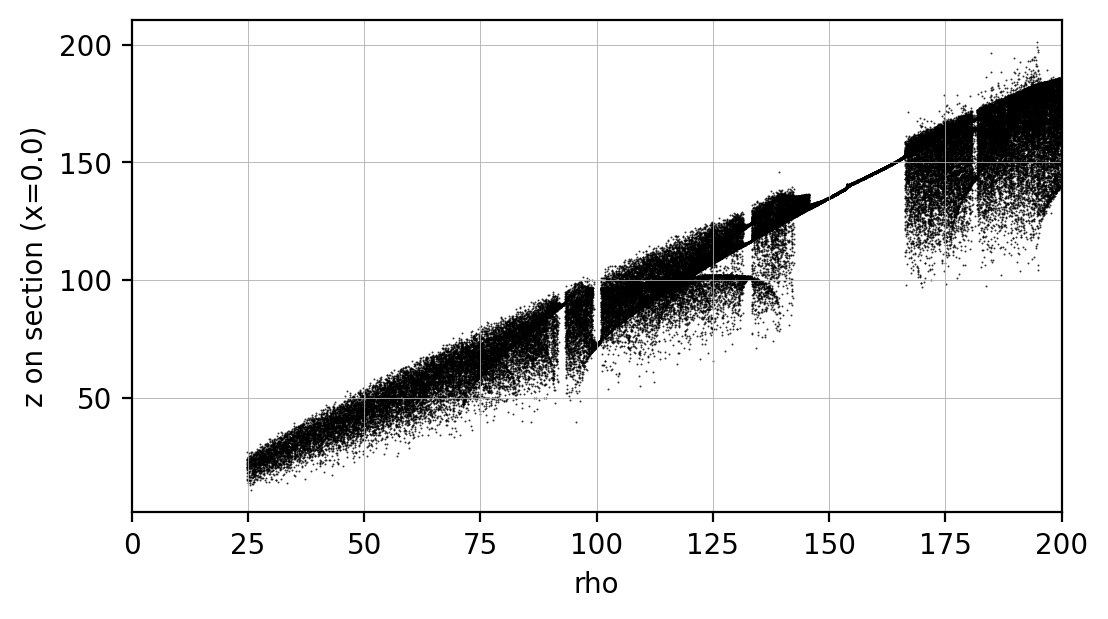
\includegraphics[width=0.58\textwidth]{lorenz_bif_rho.png}
  \caption{Παραμετρική ανάλυση του συστήματος Lorenz ως προς την παράμετρο $\rho$ (επάνω).}
  \label{fig:lorenz-bif-lyap-rho}
\end{figure}

Στο επόμενο σχήμα δίνεται το αντίστοιχο διάγραμμα μέγιστου εκθέτη Lyapunov.

\begin{figure}[H]
  \centering
  \includegraphics[width=0.58\textwidth]{lya_lorenz_rho.png}
  \caption{
  (κάτω) Αντίστοιχο διάγραμμα μέγιστου εκθέτη Lyapunov,
  το οποίο ποσοτικοποιεί τη μετάβαση από περιοδική σε χαοτική δυναμική.
  Η συμφωνία μεταξύ των δύο διαγραμμάτων αναδεικνύει τη συνέπεια
  μεταξύ ποιοτικής και ποσοτικής ανάλυσης.
  }
  \label{fig:lorenz-lyap-rho}
\end{figure}

Στα Σχ.~\ref{fig:lorenz-bif-lyap-rho} και~\ref{fig:lorenz-lyap-rho} παρουσιάζονται
αντίστοιχα το διάγραμμα διακλάδωσης και το διάγραμμα μέγιστου εκθέτη Lyapunov
ως προς την παράμετρο $\rho$,
επιτρέποντας άμεση συσχέτιση γεωμετρικών και δυναμικών χαρακτηριστικών.


\section{Υπολογισμός εκθετών Lyapunov}

\subsection{Γραμμικοποίηση, παραγώγος ροής και εξισώσεις μεταβολής}
Για την τροχιά αναφοράς $\mathbf{x}(t)=\phi_t(\mathbf{x}_0)$, μια απειροστή διαταραχή $\delta\mathbf{x}(t)$ εξελίσσεται κατά προσέγγιση ως
\begin{equation}
\dot{\delta\mathbf{x}} = J(\mathbf{x}(t),t)\,\delta\mathbf{x},
\qquad
J(\mathbf{x},t)=\frac{\partial \mathbf{f}}{\partial \mathbf{x}}(\mathbf{x},t).
\end{equation}
Ισοδύναμα, η τοπική συμπεριφορά της ροής περιγράφεται από την παραγώγο ροής
$D\phi_t(\mathbf{x}_0)$.
Δηλαδή, η παράγωγος ροής ισοδυναμεί με τον Ιακωβιανό της λύσης ως προς τις
αρχικές συνθήκες και ικανοποιεί τις εξισώσεις μεταβολής.
\begin{equation}
D\phi_t(\mathbf{x}_0)=\frac{\partial \phi_t(\mathbf{x}_0)}{\partial \mathbf{x}_0}\in\mathbb{R}^{n\times n}.
\end{equation}
Άρα ναι: ο πίνακας αυτός χαρτογραφεί μια μικρή αρχική διαταραχή
$\delta\mathbf{x}_0$ στη διαταραχή τη χρονική στιγμή $t$:
\begin{equation}
\delta\mathbf{x}(t)\approx D\phi_t(\mathbf{x}_0)\,\delta\mathbf{x}_0.
\end{equation}
Διαισθητικά:
\begin{equation}
\mathbf{x}_0 \xrightarrow{\;\phi_t\;} \mathbf{x}(t),\qquad
\mathbf{x}_0+\delta\mathbf{x}_0 \xrightarrow{\;\phi_t\;} \mathbf{x}(t)+\delta\mathbf{x}(t).
\end{equation}
Οι εκθέτες Lyapunov αντιστοιχούν στους ασυμπτωτικούς ρυθμούς μεγέθυνσης των ιδιοδιευθύνσεων της συνεπαγόμενης ροής στο εφαπτόμενο δεσμικό χώρο.

\subsection{Διευρυμένο σύστημα και υπολογισμός φάσματος}
Εξετάζουμε πίνακα εφαπτόμενων διαταραχών $Y(t)\in\mathbb{R}^{n\times n}$ με αρχική συνθήκη $Y(t_0)=I$ και
\begin{equation}
\dot{Y} = J(\mathbf{x}(t),t)\,Y.
\end{equation}
Το διευρυμένο σύστημα
\begin{equation}
\begin{cases}
\dot{\mathbf{x}} = \mathbf{f}(\mathbf{x},t),\\
\dot{Y} = J(\mathbf{x}(t),t)\,Y,
\end{cases}
\end{equation}
\paragraph{Μικροπαράδειγμα 2x2 για τις εξισώσεις μεταβολής (Duffing χωρίς απόσβεση).}
Θεωρούμε το σύστημα
\begin{equation}
\dot{x}_1=x_2,\qquad
\dot{x}_2=x_1-x_1^3.
\end{equation}
Με τη σύμβαση $J_{ij}=\partial f_i/\partial x_j$, ο Ιακωβιανός είναι
\begin{equation}
J(x_1,x_2)=
\begin{bmatrix}
0 & 1\\
1-3x_1^2 & 0
\end{bmatrix}.
\end{equation}
Θέτουμε $x(0)=(1,0)^\top$, $Y(0)=I_2$ και, για διδακτικούς λόγους, ένα βήμα Euler με $h=0.1$.
Στη χρονική στιγμή $t=0$:
\begin{equation}
J(1,0)=
\begin{bmatrix}
0 & 1\\
-2 & 0
\end{bmatrix},
\qquad
\dot{Y}(0)=J(1,0)Y(0)=
\begin{bmatrix}
0 & 1\\
-2 & 0
\end{bmatrix}.
\end{equation}
Άρα η πρώτη ενημέρωση του πίνακα μεταβολών είναι
\begin{equation}
Y(0.1)\approx Y(0)+h\dot{Y}(0)=
\begin{bmatrix}
1 & 0.1\\
-0.2 & 1
\end{bmatrix}.
\end{equation}
Ο πίνακας $Y(0.1)$ εκφράζει την πρώτη τοπική παραμόρφωση μιας αρχικής μοναδιαίας σφαίρας διαταραχών στο εφαπτόμενο επίπεδο. Με επανάληψη της ίδιας διαδικασίας και περιοδική αποσύνθεση QR αποφεύγεται η αριθμητική κατάρρευση/υπερχείλιση των στηλών του $Y$, ενώ τα $\log|R_{ii}|$ συσσωρεύονται για την εκτίμηση των εκθετών.

Στην πράξη, το παραπάνω διευρυμένο σύστημα ολοκληρώνεται αριθμητικά (με τον ίδιο ολοκληρωτή IVP, δηλαδή initial value problem), ενώ περιοδικά εφαρμόζεται ορθοκανονικοποίηση μέσω αποσύνθεσης QR (orthogonal-triangular factorization):
\begin{equation}
Y = QR.
\end{equation}
Οι εκθέτες Lyapunov προκύπτουν από τη συσσώρευση των $\ln|R_{ii}|$ κατά τη διάρκεια της φάσης μέτρησης:
\begin{equation}
\lambda_i \approx \frac{1}{T_{\mathrm{m}}}\sum_{k}\ln|R_{ii}^{(k)}|, \qquad i=1,\dots,n.
\end{equation}
Πλήρης ψευδοκωδικοποίηση της διαδικασίας (ώστε να γίνεται άμεση μετάβαση
από το κύριο κείμενο) δίνεται στο Παράρτημα~\ref{app:lyapunov},
Αλγόριθμος~\ref{alg:lyapunov-qr}.
Η υλοποίηση αντιστοιχεί σε QR-based μέθοδο (με αποσύνθεση QR) στο πνεύμα των Benettin-Shimada-Nagashima,
με τη γενική μεθοδολογία σύμφωνη με καθιερωμένες αναφορές στη βιβλιογραφία
των Lyapunov εκτιμήσεων \cite{benettin_1980,shimada_nagashima_1979,wolf_1985,dieci_vleck_2002}.

\subsection{Πρακτικό κριτήριο σύγκλισης του \texorpdfstring{$\lambda_{\max}$}{lambda\_max} που εφαρμόστηκε}
Στα πειράματα σύγκλισης του έργου, προς επιβεβαίωση των δυναμικών συστημάτων που
παρουσιάζονται στις εργασίες \cite{pham2014_no_equilibrium,pham2017_rounded_square,
volos2016_hidden_sync,pham2016_hyperjerk_memristive,volos2016_hindmarsh_sync,
wang2017_four_wing} (με αντιστοίχιση δοκιμών 3, 4, 5, 6, 8 και 13 αντίστοιχα),
η αξιολόγηση έγινε από την
καμπύλη $\lambda_{\max}(t_f)$ με σταθερό βήμα ολοκλήρωσης $\Delta t=0.01$.
Για κάθε configuration, ο τελικός χρόνος αυξάνεται προοδευτικά μέχρι
\begin{equation}
t_f^{\max}=2\times 10^5,
\end{equation}
ή έως ότου εμφανιστεί πλατώ στο 3ο δεκαδικό για τουλάχιστον τρία
διαδοχικά δείγματα. Ισοδύναμα, αν
$\widetilde\lambda_k=\mathrm{round}(\lambda_{\max}(t_{f,k}),3)$,
το κριτήριο πρόωρου τερματισμού είναι
\begin{equation}
\widetilde\lambda_k=\widetilde\lambda_{k+1}=\widetilde\lambda_{k+2}.
\end{equation}
Το παραπάνω κριτήριο χρησιμοποιήθηκε ως πρακτικός έλεγχος ότι οι finite-time
εκτιμήσεις έχουν σταθεροποιηθεί πριν την τελική αναφορά αποτελεσμάτων.
Δεν αποτελεί αυστηρό θεωρητικό κριτήριο σύγκλισης στο όριο $t\to\infty$, αλλά
εμπειρικό convergence monitor κατάλληλο για την κλίμακα και το είδος των συστημάτων που εξετάζονται.

\subsection{Αναλυτικός και αριθμητικός Ιακωβιανός}
\label{subsec:jacobian-analytic-fd}
\begin{definitionbox}{Αναλυτικός Jacobian και finite-difference προσέγγιση}{hairer_wanner}
Η αριθμητική υλοποίηση προϋποθέτει την αξιολόγηση του $J$ κατά μήκος της $\mathbf{x}(t)$.
Για σύστημα $\dot{\mathbf{x}}=\mathbf{f}(t,\mathbf{x})$ με $\mathbf{x}=(x_1,\dots,x_n)^\top$
και $\mathbf{f}=(f_1,\dots,f_n)^\top$, ο αναλυτικός Ιακωβιανός έχει ρητά τη μορφή
\begin{equation}
\mathbf{J}(t,\mathbf{x})=\frac{\partial \mathbf{f}}{\partial \mathbf{x}}=
\begin{bmatrix}
\dfrac{\partial f_1}{\partial x_1} & \dfrac{\partial f_1}{\partial x_2} & \cdots & \dfrac{\partial f_1}{\partial x_n} \\
\dfrac{\partial f_2}{\partial x_1} & \dfrac{\partial f_2}{\partial x_2} & \cdots & \dfrac{\partial f_2}{\partial x_n} \\
\vdots & \vdots & \ddots & \vdots \\
\dfrac{\partial f_n}{\partial x_1} & \dfrac{\partial f_n}{\partial x_2} & \cdots & \dfrac{\partial f_n}{\partial x_n}
\end{bmatrix},
\end{equation}
με στοιχεία $J_{ij}(t,\mathbf{x})=\partial f_i/\partial x_j$.
Στο παρόν εργαλείο υποστηρίζονται δύο ισοδύναμες ως προς τη θεωρία προσεγγίσεις:
\begin{itemize}
\item \textbf{Αναλυτικός Ιακωβιανός:} όταν είναι διαθέσιμη ρητή μορφή του $J(\mathbf{x},t)$, χρησιμοποιείται απευθείας στις εξισώσεις μεταβολής.
\item \textbf{Finite differences:} όταν το $J$ δεν είναι διαθέσιμο, προσεγγίζεται με κεντρικές πεπερασμένες διαφορές
\begin{equation}
J_{:,j}(\mathbf{x},t)\approx
\frac{\mathbf{f}(\mathbf{x}+\varepsilon \mathbf{e}_j,t)-\mathbf{f}(\mathbf{x}-\varepsilon \mathbf{e}_j,t)}{2\varepsilon},
\end{equation}
όπου $\varepsilon>0$ μικρή παράμετρος διακριτοποίησης και $\mathbf{e}_j$ το $j$-οστό μοναδιαίο διάνυσμα.
\end{itemize}
\end{definitionbox}
Στην πράξη, ο Jacobian με κεντρικές διαφορές απαιτεί $2n$ αξιολογήσεις του RHS (right-hand side) ανά εκτίμηση,
άρα το κόστος κλιμακώνεται ως $O(n\,\mathrm{cost}(f))$ ανά χρονική θέση όπου απαιτείται ο $J$.
Επιπλέον, η επιλογή του $\varepsilon$ είναι κρίσιμη: πολύ μικρό $\varepsilon$ ενισχύει αριθμητικό θόρυβο
(σφάλματα στρογγυλοποίησης), ενώ πολύ μεγάλο $\varepsilon$ αυξάνει το σφάλμα αποκοπής.
Και στις δύο περιπτώσεις εφαρμόζεται η ίδια διαδικασία ολοκλήρωσης, QR-ορθοκανονικοποίησης και κανονικοποίησης ως προς τον χρόνο μέτρησης.
Η επιλογή Jacobian επηρεάζει κυρίως το υπολογιστικό κόστος και την ακρίβεια της γραμμικοποίησης, όχι τη θεωρητική εγκυρότητα της μεθόδου.

\subsection{Ορισμός εκθετών Lyapunov}

\begin{definitionbox}{Εκθέτες Lyapunov (ασυμπτωτικός ορισμός και QR ισοδύναμη μορφή)}{benettin_1980,shimada_nagashima_1979,wolf_1985,dieci_vleck_2002}
Θεωρούμε $n$-διάστατο δυναμικό σύστημα συνεχούς χρόνου
\begin{equation}
\dot{\mathbf{x}} = \mathbf{f}(t,\mathbf{x}), \qquad \mathbf{x}\in\mathbb{R}^n .
\end{equation}
Οι αντίστοιχες εξισώσεις μεταβολής, οι οποίες περιγράφουν την εξέλιξη απειροστά μικρών διαταραχών της τροχιάς αναφοράς $\delta\mathbf{x}$ δίνονται από
\begin{equation}
\dot{\delta\mathbf{x}} = \mathbf{J}(t,\mathbf{x})\,\delta\mathbf{x},
\end{equation}
όπου $\mathbf{J}(t,\mathbf{x}) = \partial \mathbf{f}/\partial \mathbf{x}$ ο Jacobian πίνακας.

Οι εκθέτες Lyapunov $\lambda_i$ ορίζονται ως τα όρια για μεγάλους χρόνους (ή μαθηματικά και όχι υπολογιστικά ως ασυμπτωτικά όρια για $\lim_{t \to \infty}$
\begin{equation}
\lambda_i =
\lim_{T\to\infty}
\frac{1}{T}
\log
\frac{\|\delta\mathbf{x}_i(T)\|}{\|\delta\mathbf{x}_i(0)\|},
\qquad i=1,\dots,n ,
\end{equation}
και ποσοτικοποιούν τους μέσους εκθετικούς ρυθμούς εξέλιξης ανεξάρτητων διευθύνσεων στο εφαπτόμενο επίπεδο.
Διαισθητικά, αν δύο τροχιές ξεκινούν σε πολύ μικρή αρχική απόσταση,
τότε για μεγάλο χρόνο η απόστασή τους συμπεριφέρεται περίπου ως
\begin{equation}
\|\delta \mathbf{x}(t)\|\approx e^{\lambda t}\,\|\delta \mathbf{x}(0)\|.
\end{equation}
Άρα $\lambda>0$ σημαίνει εκθετική απόκλιση, $\lambda<0$ εκθετική σύγκλιση και $\lambda=0$ ουδέτερη (μη εκθετική) συμπεριφορά.

Στις αριθμητικές υλοποιήσεις με περιοδική ορθοκανονικοποίηση, ο παραπάνω ορισμός γράφεται ισοδύναμα ως
\begin{equation}
\lambda_i =
\lim_{T\to\infty}
\frac{1}{T}
\sum_{k=1}^{N(T)} \log \left| R^{(k)}_{ii} \right|,
\end{equation}
όπου $R^{(k)}_{ii}$ δηλώνει το $i$-ο διαγώνιο στοιχείο του άνω τριγωνικού πίνακα $\mathbf{R}$ ο οποίος προκύπτει από την $k$-η αποσύνθεση QR, και $N(T)$ είναι ο αριθμός των βημάτων ορθοκανονικοποίησης έως τον χρόνο $T$.
\end{definitionbox}

Το ακόλουθο σχήμα συνοψίζει οπτικά την έννοια της τοπικής απόκλισης/σύγκλισης τροχιών που μετρά ο εκθέτης Lyapunov.

\begin{figure}[H]
\centering
\begin{subfigure}{0.31\textwidth}
  \centering
  \includegraphics[width=\textwidth]{screenshots/LyapunovDiagram.svg.png}
  \caption{Γεωμετρική απόκλιση γειτονικών τροχιών.}
  \label{fig:lyapunov-intuition-a}
\end{subfigure}
\hfill
\begin{subfigure}{0.31\textwidth}
  \centering
  \includegraphics[width=\textwidth]{screenshots/Lyapunov-exponent.svg1.png}
  \caption{Ελλειψοειδής παραμόρφωση στο εφαπτόμενο επίπεδο.}
  \label{fig:lyapunov-intuition-b}
\end{subfigure}
\hfill
\begin{subfigure}{0.31\textwidth}
  \centering
  \includegraphics[width=\textwidth]{screenshots/Orbital_instability_(Lyapunov_exponent).png}
  \caption{Η σχέση \(\|\delta\mathbf{x}(t)\|\sim e^{\lambda t}\|\delta\mathbf{x}(0)\|\).}
  \label{fig:lyapunov-intuition-c}
\end{subfigure}
\caption{Διαισθητική οπτικοποίηση του εκθέτη Lyapunov: τοπική εξέλιξη μικρής διαταραχής και εκθετικός ρυθμός μεταβολής της απόστασης γειτονικών τροχιών (προσαρμογή από \cite{wikipedia_lyapunov_exponent}).}
\label{fig:lyapunov-intuition}
\end{figure}

\begin{theorembox}{Oseledets (Multiplicative Ergodic Theorem)}{oseledets_scholarpedia}
Έστω δυναμικό σύστημα με αμετάβλητο εργοδικό μέτρο και κατάλληλες συνθήκες ολοκληρωσιμότητας για την παραγώγο ροής.
Τότε, για σχεδόν κάθε αρχική συνθήκη, υπάρχουν πραγματικοί εκθέτες
\(\lambda_1 \ge \lambda_2 \ge \dots \ge \lambda_n\) και αντίστοιχη διάσπαση του εφαπτόμενου χώρου σε Oseledets υποχώρους,
ώστε οι ασυμπτωτικοί ρυθμοί μεγέθυνσης των διαταραχών να υπάρχουν και να ισούνται με αυτούς τους εκθέτες.
\end{theorembox}

\begin{definitionbox}{Oseledets υποχώροι (Lyapunov διευθύνσεις)}{oseledets_scholarpedia}
Για σχεδόν κάθε σημείο $\mathbf{x}$, ο εφαπτόμενος χώρος διασπάται ως
\begin{equation}
T_{\mathbf{x}}M = E_1(\mathbf{x}) \oplus E_2(\mathbf{x}) \oplus \cdots \oplus E_k(\mathbf{x}),
\end{equation}
όπου κάθε $E_i(\mathbf{x})$ είναι Oseledets υποχώρος που αντιστοιχεί στον εκθέτη $\lambda_i$.
Ισοδύναμα, για κάθε μη μηδενικό $\mathbf{v}\in E_i(\mathbf{x})$ ισχύει
\begin{equation}
\lim_{t\to\infty}\frac{1}{t}\log\!\left\|D\Phi^t_{\mathbf{x}}\,\mathbf{v}\right\|=\lambda_i.
\end{equation}
Άρα οι Oseledets υποχώροι είναι οι γεωμετρικές διευθύνσεις του εφαπτόμενου χώρου στις οποίες μετριούνται οι ασυμπτωτικοί ρυθμοί διαστολής/συστολής.
\end{definitionbox}

\subsection{Μικροπαράδειγμα 2D για τη συσσώρευση \texorpdfstring{$\log|R_{ii}|$}{log|Rii|}}
Θεωρούμε το γραμμικό σύστημα
\begin{equation}
\dot{\mathbf{x}}=A\mathbf{x},\qquad
A=
\begin{bmatrix}
0.2 & 0\\
0 & -0.1
\end{bmatrix}.
\end{equation}
Για αυτό το σύστημα, οι πραγματικοί εκθέτες Lyapunov είναι $\lambda_1=0.2$ και $\lambda_2=-0.1$.
Εφαρμόζουμε QR-based υπολογισμό με διάστημα ορθοκανονικοποίησης $\Delta T=1$ και $Y(0)=I$.

Σε κάθε διάστημα (interval):
\begin{equation}
Y^\star = e^{A\Delta T}=
\begin{bmatrix}
e^{0.2} & 0\\
0 & e^{-0.1}
\end{bmatrix},
\quad
Y^\star = QR,
\quad
R=
\begin{bmatrix}
e^{0.2} & 0\\
0 & e^{-0.1}
\end{bmatrix}.
\end{equation}
Άρα σε κάθε QR βήμα $k$:
\begin{equation}
\log|R_{11}^{(k)}|=0.2,\qquad \log|R_{22}^{(k)}|=-0.1.
\end{equation}
Με συσσώρευση για 4 βήματα:
\begin{equation}
S_1=\sum_{k=1}^{4}\log|R_{11}^{(k)}|=0.8,\qquad
S_2=\sum_{k=1}^{4}\log|R_{22}^{(k)}|=-0.4,\qquad
T=4.
\end{equation}
Τότε οι εκτιμήσεις είναι
\begin{equation}
\lambda_1\approx \frac{S_1}{T}=0.2,\qquad
\lambda_2\approx \frac{S_2}{T}=-0.1.
\end{equation}
Δηλαδή, το QR algorithm κάνει ακριβώς αυτό που περιγράφει ο τύπος:
σε κάθε διάστημα προσθέτει $\log|R_{ii}|$ και στο τέλος διαιρεί με τον συνολικό χρόνο μέτρησης.

\subsection{Εμπειρικοί κανόνες ερμηνείας του φάσματος Lyapunov}
Για πρακτική ερμηνεία των αποτελεσμάτων, χρησιμοποιούνται συχνά οι παρακάτω
κανόνες (ως ένδειξη, όχι ως απόλυτο κριτήριο):
\begin{itemize}
  \item \textbf{Χάος:} ύπαρξη τουλάχιστον ενός θετικού εκθέτη ($\lambda_1>0$).
  \item \textbf{Τυπικό αυτόνομο σύστημα με χαοτικό ελκυστή:}
  ένας θετικός, ένας περίπου μηδενικός (λόγω χρονικής μετατόπισης της ροής), και οι υπόλοιποι αρνητικοί.
  \item \textbf{Υπερχαοτική συμπεριφορά (hyperchaos):}
  τουλάχιστον δύο θετικοί εκθέτες ($\lambda_1>0,\lambda_2>0$), που δηλώνουν εκθετική απόκλιση σε δύο ανεξάρτητες διευθύνσεις.
  \item \textbf{Περιοδική τροχιά:} ένας εκθέτης περίπου μηδενικός και οι υπόλοιποι αρνητικοί.
  \item \textbf{Ισορροπία (σταθερό fixed point):} όλοι αρνητικοί.
  \item \textbf{Διασπορά/συστολή όγκου:} το άθροισμα $\sum_i\lambda_i$ λειτουργεί ως δείκτης μέσης ογκομετρικής μεταβολής
  (αρνητικό: μέση συστολή, περίπου μηδενικό: σχεδόν διατήρηση όγκου).
\end{itemize}
Στην πράξη, επειδή υπολογίζονται πεπερασμένου χρόνου (\emph{finite-time}) εκτιμήσεις, οι έλεγχοι
για ``μηδενικό'' εκθέτη γίνονται με ανοχή και με επαλήθευση ως προς τη
σταθεροποίηση των τιμών όταν αυξάνεται ο χρόνος μέτρησης.

\subsection{Οπτική εξέλιξη της QR ορθοκανονικοποίησης σε run R\"ossler}
Η οπτικοποίηση προσομοιώνει άμεσα τον πυρήνα του QR-based αλγορίθμου για εκθέτες Lyapunov:
εκκινούμε από ένα ισότροπο νέφος διαταραχών (σφαιρική γεωμετρία στο εφαπτόμενο επίπεδο)
και το προωθούμε με τις εξισώσεις μεταβολής
\(\dot{\delta\mathbf{x}}=\mathbf{J}(\mathbf{x}(t),t)\,\delta\mathbf{x}\).
Η γραμμικοποιημένη ροή παραμορφώνει τη σφαίρα σε ελλειψοειδές και τείνει να ευθυγραμμίσει
τις διαταραχές προς τη διεύθυνση μέγιστης διαστολής (κυριαρχία του μεγαλύτερου εκθέτη).

Για να αποφευχθεί αυτή η αριθμητική εκφύλιση της βάσης, εφαρμόζεται περιοδικά
αποσύνθεση QR: το \(\mathbf{Q}\) επαναφέρει ορθοκανονικό πλαίσιο (γεωμετρικά:
επιστροφή σε σφαιρική κατανομή), ενώ το \(\mathbf{R}\) αποθηκεύει τους τοπικούς
συντελεστές διαστολής/συστολής. Έτσι, το reset της γεωμετρίας δεν χάνει πληροφορία:
η πληροφορία συσσωρεύεται στους όρους \(\sum_k \log|R_{ii}^{(k)}|\), από όπου
υπολογίζονται οι εκθέτες Lyapunov.

Στα παρακάτω καρέ, αριστερά φαίνεται το QR reset (pre\_qr σε πορτοκαλί, post\_qr σε μπλε)
και δεξιά το Lyapunov-expanded post mesh.

\begin{figure}[H]
\centering
\begin{subfigure}[t]{0.499\textwidth}
  \centering
  \includegraphics[width=\textwidth,trim=90 70 90 55,clip]{figures/frame_000_delay-1s.png}
  \caption{chunk=1}
  \label{fig:ch1-cpp-qr-frames-top-1}
\end{subfigure}%
\begin{subfigure}[t]{0.499\textwidth}
  \centering
  \includegraphics[width=\textwidth,trim=90 70 90 55,clip]{figures/frame_001_delay-1s.png}
  \caption{chunk=101}
  \label{fig:ch1-cpp-qr-frames-top-2}
\end{subfigure}
\vspace{0.25em}
\begin{subfigure}[t]{0.78\textwidth}
  \centering
  \includegraphics[width=\textwidth,trim=90 70 90 55,clip]{figures/frame_002_delay-1s.png}
  \caption{chunk=201}
  \label{fig:ch1-cpp-qr-frames-top-3}
\end{subfigure}
\caption{Σχήμα 1.10: εξέλιξη της QR ορθοκανονικοποίησης (πρώτη τριάδα καρέ).
Οι τιμές \(\boldsymbol{\lambda}\) που αναγράφονται στα καρέ μεταβαίνουν από
\([0.0204,\,0.1784,\,-12.7495]\) σε
\([0.1056,\,0.0344,\,-6.6062]\) και
\([0.1011,\,0.0325,\,-7.4923]\), δείχνοντας τη μετάβαση από ισχυρό transient
σε πιο σταθερή φασματική συμπεριφορά. Πηγή καρέ: \cite{gkountinakos_chaos_trace_cpp_2026}.}
\label{fig:ch1-cpp-qr-frames-top}
\end{figure}

Στη δεύτερη τριάδα καρέ, η ίδια διαδικασία σε μεταγενέστερο χρόνο δείχνει
προσέγγιση του τυπικού προτύπου για χαοτική αυτόνομη ροή:
\(\lambda_1>0\), \(\lambda_2\approx 0\), \(\lambda_3<0\).

\begin{figure}[H]
\centering
\begin{subfigure}[t]{0.499\textwidth}
  \centering
  \includegraphics[width=\textwidth,trim=90 70 90 55,clip]{figures/frame_003_delay-1s.png}
  \caption{chunk=301}
  \label{fig:ch1-cpp-qr-frames-bottom-1}
\end{subfigure}%
\begin{subfigure}[t]{0.499\textwidth}
  \centering
  \includegraphics[width=\textwidth,trim=90 70 90 55,clip]{figures/frame_004_delay-1s.png}
  \caption{chunk=401}
  \label{fig:ch1-cpp-qr-frames-bottom-2}
\end{subfigure}
\vspace{0.25em}
\begin{subfigure}[t]{0.78\textwidth}
  \centering
  \includegraphics[width=\textwidth,trim=90 70 90 55,clip]{figures/frame_005_delay-1s.png}
  \caption{chunk=501}
  \label{fig:ch1-cpp-qr-frames-bottom-3}
\end{subfigure}
\caption{Σχήμα 1.11: εξέλιξη της QR ορθοκανονικοποίησης (δεύτερη τριάδα καρέ).
Οι ενδεικτικές τιμές \(\boldsymbol{\lambda}\) είναι
\([0.1105,\,-0.0077,\,-7.3025]\),
\([0.1027,\,0.0080,\,-7.1033]\),
\([0.1183,\,0.0142,\,-7.2031]\).
Η δεύτερη τιμή παραμένει κοντά στο μηδέν, ενώ η πρώτη θετική και η τρίτη αρνητική,
όπως αναμένεται για το χαοτικό καθεστώς του R\"ossler. Πηγή καρέ: \cite{gkountinakos_chaos_trace_cpp_2026}.}
\label{fig:ch1-cpp-qr-frames-bottom}
\end{figure}


\subsection{Πειραματική αξιολόγηση επιλογής QR period (περιόδου ορθοκανονικοποίησης) με heatmaps}
\label{sec:ch1-qr-period-study}

Για να συνδεθεί ο θεωρητικός ορισμός του φάσματος Lyapunov με πρακτικό, αναπαραγώγιμο
κριτήριο ρύθμισης, εκτελέστηκε ανεξάρτητη μελέτη με σταθερά $\Delta t$, $T_{\mathrm{tr}}$,
$T_{\mathrm{meas}}$ και \textbf{μονοπαραμετρικό sweep στο σύστημα Rössler}.
Ως reference χρησιμοποιήθηκε το $\mathrm{qr\_every\_steps}=1$,
ενώ για κάθε επιλογή QR period (περιόδου ορθοκανονικοποίησης) καταγράφηκαν:
\begin{itemize}
  \item το μέγιστο απόλυτο σφάλμα ως προς reference,
  \item δείκτης χρονικής σταθερότητας των running εκτιμήσεων.
\end{itemize}

Το γράφημα της Εικόνας~\ref{fig:ch1-qr-accuracy-stability} δίνει τη συνολική τάση σφάλματος/σταθερότητας
ως συνάρτηση του QR period (περιόδου ορθοκανονικοποίησης) και λειτουργεί ως πρώτο φίλτρο επιλογής.

Στο επόμενο σχήμα φαίνονται οι καμπύλες σφάλματος και σταθερότητας σε συνάρτηση με την περίοδο της ορθοκανονικοποίησης
-ανά πόσα χρονικά βήματα συμβαίνει- \texttt{qr\_every\_steps}.

\begin{figure}[H]
\centering
\includegraphics[width=0.94\textwidth]{\lyastudyfigdir/accuracy_stability_vs_qr.png}
\caption{Καμπύλες ακρίβειας και σταθερότητας έναντι του $\mathrm{qr\_every\_steps}$.
Αριστερά: μέσο και μέγιστο σφάλμα ως προς reference ($\mathrm{qr}=1$).
Δεξιά: μέσος και μέγιστος δείκτης χρονικής σταθερότητας των running Lyapunov εκτιμήσεων.}
\label{fig:ch1-qr-accuracy-stability}
\end{figure}

Οι heatmaps της Εικόνας~\ref{fig:ch1-qr-heatmaps} είναι το κρίσιμο δεύτερο επίπεδο ανάλυσης,
επειδή δείχνουν την ποιότητα του ίδιας περιόδου ορθοκανονικοποίησης σε όλο το sweep παραμέτρου (και όχι μόνο
σε μια συνολική τιμή):
\begin{itemize}
  \item στον heatmap σφάλματος αναζητούμε ζώνες χαμηλών τιμών σε όσο το δυνατόν μεγαλύτερο τμήμα του sweep,
  \item στον heatmap σταθερότητας αναζητούμε ταυτόχρονα ομαλή/σταθερή συμπεριφορά των running εκτιμήσεων,
  \item πρακτικά αποδεκτή επιλογή QR period (περιόδου ορθοκανονικοποίησης) είναι εκείνη που παραμένει χαμηλή και στα δύο κριτήρια,
  ώστε να αποφεύγονται τιμές που φαίνονται καλές τοπικά αλλά αποσταθεροποιούνται σε άλλη περιοχή παραμέτρων.
\end{itemize}

Ακολουθούν θερμικοί χάρτες που συνοψίζουν σφάλμα και σταθερότητα Lyapunov σε όλο το sweep παραμέτρου.

\begin{figure}[H]
\centering
\begin{subfigure}[t]{0.49\textwidth}
\centering
\includegraphics[width=\textwidth]{\lyastudyfigdir/heatmap_max_abs_err.png}
\caption{Heatmap μέγιστου απόλυτου σφάλματος ως προς reference.}
\label{fig:ch1-qr-heatmap-err}
\end{subfigure}
\hfill
\begin{subfigure}[t]{0.49\textwidth}
\centering
\includegraphics[width=\textwidth]{\lyastudyfigdir/heatmap_max_stability.png}
\caption{Heatmap δείκτη χρονικής σταθερότητας των running εκθετών.}
\label{fig:ch1-qr-heatmap-stab}
\end{subfigure}
\caption{Θερμικοί χάρτες ποιότητας υπολογισμού Lyapunov ως προς QR period (περίοδο ορθοκανονικοποίησης) και παράμετρο συστήματος.
Ο συνδυασμός τους επιτρέπει επιλογή QR period (περιόδου ορθοκανονικοποίησης) που παραμένει αριθμητικά αξιόπιστο σε όλο το sweep.}
\label{fig:ch1-qr-heatmaps}
\end{figure}

\chapter{Υπολογιστική και Προγραμματιστική Υλοποίηση του Προσομοιωτή}
\label{ch:computational-implementation}

\noindent\textbf{Chapter summary.}
\textenglish{
This chapter documents the software and computational implementation of the simulator as an executable research system, based on the actual codebase, internal technical notes, and benchmarking scripts. Its primary objective is to map user-facing actions to numerical execution paths, clarify component responsibilities, and make implementation decisions auditable from both a software engineering and numerical analysis perspective.

The chapter describes the runtime stack (Python, Streamlit, NumPy, SciPy, SymPy, Matplotlib, Numba) and presents a three-layer architecture: interface components for experiment configuration, controller/orchestration logic for validation and workflow control, and a numerical core for integration, Poincaré processing, Lyapunov estimation, and sweep accumulation. It explains how data and parameters propagate across these layers, how state is persisted for repeatable experiments, and how exported artifacts are generated.

A dedicated part of the chapter focuses on acceleration strategy. It details when just-in-time compilation is enabled, how Numba kernels are specialized and cached, why fallbacks are required for unsupported execution paths, and how this hybrid model balances performance with maintainability. The text also contrasts interpreted Python execution with compiled alternatives, including practical trade-offs related to overhead, memory movement, extensibility, and operational complexity.

Finally, the chapter provides implementation-level reproducibility guidance: equation parsing conventions, solver and tolerance controls, transient/measurement configuration, QR scheduling parameters, benchmarking protocol, and backend comparison methodology. Complexity and runtime sections connect algorithmic costs to observed wall-time behavior, so reported performance claims remain traceable to concrete workload definitions. In that sense, Chapter 2 functions as both a technical manual for the platform and a reproducibility framework for the experiments reported in this thesis.
}

\vspace{8pt}

\section{Σκοπός του κεφαλαίου}

Το παρόν κεφάλαιο επιχειρεί να αναλύσει τον τρόπο λειτουργίας
κάθε feature - επιλογής, στην εφαρμογή και στα συνοδευτικά της notebooks
όπως είσης και να τεκμηριώσει, σε υπολογιστικό επίπεδο και σε επίπεδο μηχανικής
λογισμικού, την υλοποίηση του \textit{DynaSim - Non-Linear Dynamical Systems Simulator} (Streamlit εφαρμογή για
μη γραμμικά δυναμικά συστήματα). Η περιγραφή βασίζεται στο πραγματικό
codebase και στα συνοδευτικά έγγραφα docs και ReadMes. \cite{nlds_internal_md_docs}:

Ο στόχος είναι διπλός:
\begin{itemize}
\item να χαρτογραφηθεί επαρκώς η διαδικασία διάδρασης της διεπαφή χρήστη με τον αριθμητικό πυρήνα,
\item να προσδιοριστεί σαφώς ο ρόλος κάθε συστατικού κορμού του λογισμικού και να διευκολυνθεί η ανακυκλωσιμότητα και η επέκτασιμότητα της εφαρμογής,
\item να αναλυθεί η υπολογιστική πολυπλοκότητα και η επιτάχυνση μέσω Numba/JIT (just-in-time).
\end{itemize}

\section{Υπολογιστικό περιβάλλον και προαπαιτούμενα}

\subsection{Βασικά εργαλεία}

Η εφαρμογή και τα συνοδευτικά notebooks έχουν υλοποιηθεί σε Python 3.10+ και βασίζονται σε ένα σύνολο βιβλιοθηκών που καλύπτουν από τη διαχείριση διεπαφής χρήστη μέχρι την αριθμητική ολοκλήρωση και την ανάλυση δεδομένων. 
Οι βιβλιοθήκες που απαιτούνται γαι την υλοποίηση παρουσιάζονται στον Πίνακα~\ref{tab:ch2-stack}.

\begin{table}[H]
\centering
\caption{Οι βιβλιοθήκες που χρησιμοποιούνται στην υλοποίηση του DynaSim}
\label{tab:ch2-stack}
\renewcommand{\arraystretch}{1.15}
\begin{tabular}{|l|p{0.64\textwidth}|}
\hline
\textbf{Συστατικό} & \textbf{Ρόλος στην υλοποίηση} \\
\hline
Python & Κεντρική γλώσσα υλοποίησης (UI (user interface), orchestration, numerics, exports). \\
\hline
Streamlit & Διαδραστική διεπαφή, tabs, stateful widgets και workflow ελέγχου. \\
\hline
NumPy & Διανυσματική αριθμητική, πίνακες κατάστασης/τροχιάς. \\
\hline
SciPy (\texttt{solve\_ivp}) & Προσαρμοστικοί ολοκληρωτές RK45/DOP853 και event detection. \\
\hline
SymPy & Parsing custom εξισώσεων, συμβολικός Jacobian, expression-based τομές. \\
\hline
Numba & JIT (just-in-time) επιτάχυνση fixed-step RK4, Forest-Ruth και Lyapunov loops. \\
\hline
Pandas & Δομές δεδομένων για sweeps και εξαγωγές CSV (comma-separated values). \\
\hline
Matplotlib & Παραγωγή διαγραμμάτων φάσης, χρονοσειρών, διακλάδωσης, Lyapunov. \\
\hline
\end{tabular}
\end{table}

Η τεχνολογική στοίβα περιλαμβάνει επίσης
\texttt{psutil} για πληροφορίες συστήματος που σχετίζονται με python workers, ώστε να επιτρέπει την παρακολούθηση των πόρων 
και την αποτελεσματική παραλληλοποίηση των εργασιών που υποστηρίζονται.

\subsection{Αρχιτεκτονική τριών επιπέδων}
\label{subsec:three-layer-architecture}

\begin{importantbox}
Η υλοποίηση ακολουθεί τον παρακάτω διαχωρισμό:
\begin{itemize}
\item \textbf{UI layer (user interface):} \texttt{app/nlds\_app.py}, \texttt{app/ui/*}.
\item \textbf{Controller layer:} \texttt{app/cache.py}, \texttt{app/sweep.py},
\texttt{app/logic/*}.
\item \textbf{Numerical core:} \texttt{core/*}
(\texttt{solver.py}, \texttt{lyapunov.py},
\texttt{poincare\_sweep.py}, \texttt{symplectic\_solver.py},
\texttt{numba\_backend/*}).
\end{itemize}

Η διαστρωμάτωση αυτή ελαχιστοποιεί coupling διεπαφής-αλγορίθμων και επιτρέπει
αντικατάσταση backend χωρίς αλλαγές στη ροή χρήσης.
\end{importantbox}

\section{Λειτουργική ροή της εφαρμογής }

\subsection{Ορισμός συστήματος και εξισώσεων}

\begin{guidebox}
Ο χρήστης ξεκινά από το sidebar:
\begin{enumerate}
\item επιλογή κατηγορίας συστήματος (Lorenz/Rössler/Henon-Heiles/Custom),
\item επιλογή solver kind (runke kutta ή symplectic 4th order, είτε rk45/dop853 της SciPy χωρίς την χρήση Numba),
\item δήλωση αρχικών συνθηκών,
\item (για custom σύστημα) ορισμός μεταβλητών, εξισώσεων και παραμέτρων.
\end{enumerate}
\end{guidebox}

Στο ακόλουθο σχήμα παρουσιάζονται τα βασικά βήματα setup: επιλογή συστήματος, αρχικοί ή custom ορισμοί και symbolic Jacobian.

\begin{figure}[H]
\centering
\begin{subfigure}{0.32\textwidth}
  \centering
  \includegraphics[width=\textwidth]{figures/ch2/s1_system_selection.png}
  \caption{System επιλογή}
  \label{fig:ch2-s1-system}
\end{subfigure}
\hfill
\begin{subfigure}{0.32\textwidth}
  \centering
  \includegraphics[width=\textwidth]{figures/ch2/s2_initial_and_custom_definitions.png}
  \caption{Initial/Custom defs}
  \label{fig:ch2-s2-custom-def}
\end{subfigure}
\hfill
\begin{subfigure}{0.32\textwidth}
  \centering
  \includegraphics[width=\textwidth]{figures/ch2/s3_symbolic_jacobian.png}
  \caption{Symbolic Jacobian}
  \label{fig:ch2-s3-jacobian}
\end{subfigure}
\caption{Tab setup: επιλογή συστήματος, ορισμός custom εξισώσεων και Jacobian.(Παράδειγμα)}
\label{fig:ch2-tab-setup}
\end{figure}

\subsection{Ρυθμίσεις ολοκλήρωσης και οπτικοποίησης (1ο Tab )}
\label{subsec:tab1-settings}

\begin{guidebox}
Στο 1ο Tab (Phase portrait), η διαδικασία που ακολουθεί ο χρήστης περιλαμβάνει τα εξής βήματα:
\begin{enumerate}
\item ορισμός χρονικού παραθύρου ολοκλήρωσης ($t_0 (initial time)$, $t_f (final time)$, $\Delta t (time step)$),
\item επιλογή παραμέτρων συστήματος,
\item ρύθμιση transient cut και Lyapunov controls,
\item επιλογή αξόνων, ανοχών solver (μόνο για τους solver της SciPy, για τους fixed step καθορίζουμε την ακρίβεια μέσω $\Delta t$) και αποθήκευση configuration.
\item στο τέλος της σελίδας, επιλέγοντας \textit{Save Configuration} αποθηκεύεται το τρέχον configuration σε JSON (JavaScript Object Notation), το οποίο μπορεί να επαναφορτωθεί μέσω του αντίστοιχου κουμπιού στο sidebar, ή να χρησιμοποιηθεί στο αντίστοιχο notebook.
\end{enumerate}
\end{guidebox}

Ακολουθούν εικόνες με τις κύριες ρυθμίσεις ολοκλήρωσης και προβολής του 1ου Tab.

\begin{figure}[H]
\centering
\begin{subfigure}{0.47\textwidth}
  \centering
  \includegraphics[width=\textwidth]{figures/ch2/s4_integration_controls.png}
  \caption{Integration}
  \label{fig:ch2-s4-integration}
\end{subfigure}
\hfill
\begin{subfigure}{0.47\textwidth}
  \centering
  \includegraphics[width=\textwidth]{figures/ch2/s6_plot_settings_lyapunov.png}
  \caption{Plot/Lyapunov}
  \label{fig:ch2-s6-plot}
\end{subfigure}
\caption{Tab 1: συνοπτική εικόνα ρυθμίσεων ολοκλήρωσης και προβολής (πάνω σειρά).}
\label{fig:ch2-tab1}
\end{figure}


\begin{figure}[H]
\centering
\begin{subfigure}{0.32\textwidth}
  \centering
  \includegraphics[width=\textwidth]{figures/ch2/s7_axis_selection.png}
  \caption{Axes}
  \label{fig:ch2-s7-axis}
\end{subfigure}
\hfill
\begin{subfigure}{0.32\textwidth}
  \centering
  \includegraphics[width=\textwidth]{figures/ch2/s8_solver_tolerances.png}
  \caption{Tolerances}
  \label{fig:ch2-s8-tols}
\end{subfigure}
\hfill
\begin{subfigure}{0.32\textwidth}
  \centering
  \includegraphics[width=\textwidth]{figures/ch2/s9_save_configuration.png}
  \caption{Save config}
  \label{fig:ch2-s9-save}
\end{subfigure}
\caption{Tab 1: συνοπτική εικόνα επιλογής αξόνων, ανοχών solver και αποθήκευσης configuration (κάτω σειρά).}
\label{fig:ch2-tab1-bottom}
\end{figure}

\subsection{Χρονοσειρές (2o Tab)}

\begin{guidebox}
Στο 2ο Tab (Time series), ο χρήστης μπορεί να επιλέξει χρονικό παράθυρο για την απεικόνιση των χρονοσειρών,
επαναχρησιμοποιεί την ολοκλήρωση που έχει ήδη εκτελεστεί στο 1ο Tab, και να εστιάσει στην post-transient περιοχή για καλύτερη οπτικοποίηση της ασυμπτωτικής συμπεριφοράς,
εφαρμόζοντας χρονικό φίλτρο παραθύρου στην ήδη υπολογισμένη τροχιά $[t_start,t_end]$.
\end{guidebox}
Ακολουθεί το στιγμιότυπο του 2ου Tab για την επιλογή χρονικού παραθύρου στις χρονοσειρές.
\begin{figure}[H]
\centering
\includegraphics[width=0.55\textwidth]{figures/ch2/s10_time_series_window.png}
\caption{Tab 2 - Time series: επιλογή χρονικού παραθύρου.}
\label{fig:ch2-s10-ts}
\end{figure}

\subsection{Παραμετρικές σαρώσεις (3o Tab)}
\label{subsec:tab3-sweeps}

\begin{guidebox}
Το 3o Tab οργανώνεται σε δύο παράλληλες υποενότητες:

\begin{itemize}
\item \textbf{Bifurcation sweep settings} (αριστερά): τομή Poincar\'e, method, early stop, max hits.
\item \textbf{Lyapunov sweep settings} (δεξιά): QR interval, transient fraction, clip policy.
\end{itemize}
\end{guidebox}

Στις παρακάτων εικόνες παρουσιάζεται το 3o Tab με τις ρυθμίσεις των bifurcation και lyapunov exponents sweep.

\begin{figure}[H]
\centering
\begin{subfigure}{0.32\textwidth}
  \centering
  \includegraphics[width=\textwidth]{figures/ch2/s11_tab3_top_setup.png}
  \caption{Sweep setup}
  \label{fig:ch2-s11-tab3-top}
\end{subfigure}
\hfill
\begin{subfigure}{0.32\textwidth}
  \centering
  \includegraphics[width=\textwidth]{figures/ch2/s12_bifurcation_parallel_section.png}
  \caption{Bifurcation section}
  \label{fig:ch2-s12-bif-section}
\end{subfigure}
\hfill
\begin{subfigure}{0.32\textwidth}
  \centering
  \includegraphics[width=\textwidth]{figures/ch2/s13_bifurcation_method_earlystop.png}
  \caption{Bifurcation method}
  \label{fig:ch2-s13-bif-method}
\end{subfigure}
\caption{Tab 3 (Σχήμα 2.4.1): συνοπτική εικόνα ρυθμίσεων bifurcation sweep (πάνω σειρά).}
\label{fig:ch2-tab3}
\end{figure}

Ακολουθεί η κάτω σειρά του Tab 3 με τις βασικές ρυθμίσεις του Lyapunov sweep.

\begin{figure}[H]
\centering
\begin{subfigure}{0.48\textwidth}
  \centering
  \includegraphics[width=\textwidth]{figures/ch2/s14_lyapunov_sweep_settings.png}
  \caption{Lyapunov settings}
  \label{fig:ch2-s14-lya-settings}
\end{subfigure}
\hfill
\begin{subfigure}{0.48\textwidth}
  \centering
  \includegraphics[width=\textwidth]{figures/ch2/s15_lyapunov_clip_and_run.png}
  \caption{Lyapunov clip/run}
  \label{fig:ch2-s15-lya-run}
\end{subfigure}
\caption{Tab 3 (Σχήμα 2.4.2): συνοπτική εικόνα ρυθμίσεων Lyapunov sweep (κάτω σειρά).}
\label{fig:ch2-tab3-bottom}
\end{figure}

\subsection{Διαχείριση RAM και αποθήκευσης σε μεγάλα runs}
\label{subsec:ram-storage-large-runs}

Στην τρέχουσα υλοποίηση, το 1ο Tab (phase/time-series) εκτελεί την ολοκλήρωση τροχιάς
με τα τρέχοντα \((t_0,t_f,\Delta t)\) πριν από την απεικόνιση. Αυτό σημαίνει ότι αν ο
χρήστης αυξήσει πολύ το \(t_f\) (π.χ. για Lyapunov δοκιμές), ενεργοποιείται άμεσα και η
pipeline της τροχιάς/phase portrait. Για να αποφεύγονται υπερβάσεις RAM, εφαρμόζονται
ρητά όρια αποθήκευσης και decimation.

\paragraph{1) Bounded trajectory storage (στη μνήμη).}
Η ολοκλήρωση τρέχει σε όλη τη χρονική διάρκεια, αλλά ο αριθμός αποθηκευμένων δειγμάτων
περιορίζεται από \texttt{max\_store\_steps} (default: \(200{,}000\)). Με
\[
N_{\mathrm{nom}}=\Big\lfloor\frac{t_f-t_0}{\Delta t}\Big\rfloor+1,\qquad
N_{\mathrm{store}}=\min\!\left(N_{\mathrm{nom}},N_{\mathrm{store,max}}\right),
\]
όπου \(N_{\mathrm{store,max}}\) είναι το όριο \texttt{max\_store\_steps} της διεπαφής.
Η κύρια μνήμη εξόδου της τροχιάς κλιμακώνεται ως
\[
M_{\mathrm{traj,out}} \approx 8\,(n+1)\,N_{\mathrm{store}}\ \text{bytes},
\]
(\(t\) + \(n\) μεταβλητές κατάστασης, \texttt{float64}). Για Lorenz (\(n=3\)) και
\(N_{\mathrm{store}}=200{,}000\), το raw array footprint είναι περίπου \(6.1\) MiB.

\paragraph{2) Decimation για plotting.}
Τα plots δεν χρησιμοποιούν όλα τα αποθηκευμένα δείγματα: εφαρμόζεται ομοιόμορφο
downsampling σε \texttt{max\_plot\_points} (default: \(120{,}000\) για trajectory plots).
Άρα η μνήμη απεικόνισης παραμένει επίσης φραγμένη:
\[
N_{\mathrm{plot}}=\min\!\left(N_{\mathrm{store}},N_{\mathrm{plot,max}}\right),\qquad
M_{\mathrm{plot}} \approx 8\,(n+1)\,N_{\mathrm{plot}}.
\]
Εδώ \(N_{\mathrm{plot,max}}\) αντιστοιχεί στο \texttt{max\_plot\_points}.
Σημαντικό: το decimation μειώνει κυρίως κόστος render/transfer, όχι τον αριθμητικό
χρόνο ολοκλήρωσης.

\paragraph{3) Chunked export για trajectories.}
Στο export τροχιάς, αν οι γραμμές είναι πολλές, η εξαγωγή γίνεται σε chunks αντί για
ένα ενιαίο μεγάλο CSV σε μνήμη (όρια \texttt{DIRECT\_CSV\_MAX\_ROWS} και
\texttt{EXPORT\_CHUNK\_ROWS\_DEFAULT}). Έτσι αποφεύγονται προσωρινές κορυφές RAM κατά
την παραγωγή αρχείων.

\paragraph{4) Bounded-memory sweeps στο 3ο Tab.}
Για bifurcation sweeps εφαρμόζεται budget γραμμών
\texttt{MAX\_SWEEP\_ROWS\_BUDGET} (\(=300{,}000\)) και προσαρμογή
\texttt{max\_hits\_effective}\(\le \lfloor 300{,}000/P \rfloor\). Παράλληλα, τα sweep plots
decimate σε έως \(200{,}000\) σημεία. Για Lyapunov sweep αποθηκεύονται κυρίως
\((\mu_i,\lambda_1,\ldots,\lambda_n)\) ανά τιμή παραμέτρου (και όχι πλήρεις τροχιές
στη διεπαφή), άρα η μνήμη κλιμακώνεται πρακτικά ως \(O(Pn)\).

\begin{importantbox}
Τα παραπάνω όρια ελέγχουν τη μνήμη αποθήκευσης/οπτικοποίησης και σταθεροποιούν τη
συμπεριφορά σε Streamlit Cloud. Δεν μειώνουν γραμμικά τον χρόνο CPU των αριθμητικών
βρόχων όταν το \(t_f\) είναι πολύ μεγάλο.
\end{importantbox}

\begin{table}[H]
\centering
\caption{Ενδεικτικός πίνακας benchmark RAM για Lorenz long runs (\texttt{bounded\_200000}), από το notebook \texttt{tests/benchmark\_lorenz\_longruns\_ram\_vs\_steps.ipynb}.}
\label{tab:ch2-ram-ceiling-benchmark}
\renewcommand{\arraystretch}{1.12}
\begin{tabular}{|r|r|r|r|}
\hline
\textbf{\(n_{\mathrm{steps}}\)} & \textbf{stored samples} & \textbf{peak RSS [MB]} & \textbf{\(\Delta\)peak [MB]} \\
\hline
5,500,000 & 200,000 & 210.891 & 0.0039 \\
7,500,000 & 200,000 & 210.875 & 0.0039 \\
9,000,000 & 200,000 & 210.867 & 0.0039 \\
10,000,000 & 200,000 & 210.871 & 0.0078 \\
\hline
\multicolumn{4}{|p{0.86\linewidth}|}{\textbf{Παρατήρηση:} παρότι τα βήματα αυξάνουν από \(5.5\times10^6\) σε \(1.0\times10^7\), το peak RSS παραμένει πρακτικά σταθερό (\(\approx 210.86{-}210.89\) MB), επιβεβαιώνοντας ότι το όριο \texttt{max\_store\_steps} συγκρατεί τη RAM χωρίς πρόσθετη επιβάρυνση στην υλοποίηση.} \\
\hline
\end{tabular}
\end{table}

\section{Αριθμητικές μέθοδοι που υλοποιούνται}

\subsection{Ολοκλήρωση ODE (ordinary differential equation)}
\label{subsec:ode-integration-impl}

Υποστηρίζονται:
\begin{itemize}
\item RK45 (adaptive, \texttt{solve\_ivp}),
\item DOP853 (adaptive υψηλής τάξης),
\item RK4 fixed-step,
\item Symplectic Forest-Ruth 4ης τάξης για separable Hamiltonians.
\end{itemize}

Για συμπλεκτικούς ολοκληρωτές απαιτείται state της μορφής
$[q_1,\dots,q_m,p_1,\dots,p_m]$ με εξισώσεις
$\dot{q}=g(p)$ και $\dot{p}=h(q)$.

\subsection{Τομές Poincar\'e και διαγράμματα διακλάδωσης}
\label{subsec:poincare-bifurcation-impl}

Υποστηρίζονται:
\begin{itemize}
\item επίπεδο τομής: $y_{s}=v$,
\item γενική τομή έκφρασης: $g(t,y,\mu)=0$ (SymPy-backed),
\item \texttt{crossing} (αλλαγή προσήμου + γραμμική παρεμβολή),
\item \texttt{slab} ($|g|\le \mathrm{tol}$).
\end{itemize}

Στην adaptive IVP (initial value problem) περίπτωση, το \texttt{crossing} μπορεί να εκτελεστεί με
event detection (\texttt{solve\_ivp} events), μειώνοντας το κόστος σε σχέση με
την πυκνή δειγματοληψία.

\subsection{Εκτίμηση φάσματος Lyapunov}
\label{subsec:lyapunov-estimation-impl}

\begin{importantbox}
Η μεθοδολογία βασίζεται σε:
\begin{enumerate}
\item ολοκλήρωση τροχιάς $\dot{x}=f(x,t)$,
\item ολοκλήρωση εξισώσεων μεταβολής
$\dot{Q}=J(x,t)\,Q$,
\item περιοδικό QR ανά $\Delta T$,
\item συσσώρευση $\sum\log|R_{ii}|$ και κανονικοποίηση ως προς τον χρόνο μέτρησης.
\end{enumerate}

Όταν δεν υπάρχει analytic Jacobian, εφαρμόζεται προσέγγιση κεντρικών πεπερασμένων
διαφορών (central finite-differences) με βήμα \(\mathrm{fd\_eps}\). Το
\(\mathrm{fd\_eps}>0\) είναι η αριθμητική διαταραχή \(\varepsilon\) που
χρησιμοποιείται στον υπολογισμό
\begin{equation}
\frac{\partial f_i}{\partial x_j}(x,t)\approx
\frac{f_i(x+\varepsilon e_j,t)-f_i(x-\varepsilon e_j,t)}{2\varepsilon},
\quad \varepsilon=\mathrm{fd\_eps}.
\end{equation}
Στην υλοποίηση η προεπιλογή είναι \(\mathrm{fd\_eps}=10^{-8}\). Πολύ μικρή τιμή
αυξάνει τα σφάλματα στρογγύλευσης, ενώ πολύ μεγάλη τιμή αυξάνει το σφάλμα αποκοπής.
\end{importantbox}

\section{Ανάλυση πολυπλοκότητας \texorpdfstring{$O(\cdot)$}{O(.)}}
\label{sec:ch2-complexity}

\subsection{Ορισμοί συμβόλων}

\begin{table}[H]
\centering
\caption{Συμβολισμός πολυπλοκότητας για τον προσομοιωτή}
\label{tab:ch2-complexity-symbols}
\renewcommand{\arraystretch}{1.15}
\begin{tabular}{|l|p{0.64\textwidth}|}
\hline
\textbf{Σύμβολο} & \textbf{Ερμηνεία} \\
\hline
$n$ & Διάσταση κατάστασης του συστήματος. \\
\hline
$N$ & Βήματα ολοκλήρωσης σε fixed-step run, $N \approx (t_f-t_0)/\Delta t$. \\
\hline
$P$ & Πλήθος τιμών παραμέτρου σε sweep. \\
\hline
$H$ & \texttt{max\_hits} (μέγιστα hits ανά παράμετρο). \\
\hline
$C$ & Πλήθος χρονικών chunks σε event-based sweep. \\
\hline
$N_{\mathrm{QR}}$ & Πλήθος QR ορθοκανονικοποιήσεων στον Lyapunov υπολογισμό. \\
\hline
$C_f(n)$ & Κόστος μίας αξιολόγησης RHS (right-hand side) $f$. \\
\hline
$C_J(n)$ & Κόστος μίας αξιολόγησης Jacobian $J$. \\
\hline
\end{tabular}
\end{table}

\subsection{Μοναδική τροχιά (single run)}

Για fixed-step RK4:
\begin{equation}
T_{\mathrm{RK4}} = O\!\left(N \cdot C_f(n)\right),
\end{equation}
καθώς κάθε βήμα απαιτεί 4 RHS (right-hand side) evaluations (σταθερός συντελεστής).
Η μνήμη αποθήκευσης πλήρους τροχιάς είναι:
\begin{equation}
M_{\mathrm{traj}} = O(nN).
\end{equation}
Στην πρακτική υλοποίηση για cloud-safe εκτέλεση, το \(N\) αντικαθίσταται από
\(N_{\mathrm{store}}=\min(N,N_{\mathrm{store,max}})\) όταν είναι ενεργό το
\texttt{max\_store\_steps}, ώστε η in-memory αποθήκευση της τροχιάς να παραμένει φραγμένη.
Για adaptive RK45/DOP853:
\begin{equation}
T_{\mathrm{IVP}} = O\!\left(N_f \cdot C_f(n)\right),
\end{equation}
όπου \(T_{\mathrm{IVP}}\) είναι ο χρόνος επίλυσης του προβλήματος αρχικών τιμών (initial value problem).
όπου $N_f$ το πραγματικό πλήθος εσωτερικών evaluations, εξαρτώμενο από τις
ανοχές και τη δυσκαμψία της τροχιάς.

\subsection{Poincar\'e sweep}

\textbf{Κλασική fixed-step προσέγγιση:}
\begin{equation}
T_{\mathrm{sweep,classic}} = O(PN).
\end{equation}
\textbf{Event-based με chunking και early-stop:}
\begin{equation}
T_{\mathrm{sweep,event}} \approx O\!\left(P \cdot C \cdot \mathrm{cost}(\text{IVP (initial value problem) chunk})\right),
\end{equation}
με πρακτικό όφελος επειδή η συλλογή τερματίζει μόλις συμπληρωθούν τα αναγκαία
hits (\(H\)).

Μνήμη sweep (αποθήκευση μόνο plot-relevant data):
\begin{equation}
M_{\mathrm{sweep}} = O(PH).
\end{equation}
\subsection{Lyapunov φάσμα}

Με analytic Jacobian:
\begin{equation}
T_{\mathrm{lya}} =
O\!\left(N\,[C_f(n)+C_J(n)+n^3]\right)
 + O\!\left(N_{\mathrm{QR}}\,n^3\right),
\end{equation}
καθώς τόσο το \(JQ\) όσο και το QR απαιτούν κυβικό κόστος ως προς \(n\).
Εδώ, \(JQ\) είναι ο πολλαπλασιασμός του Ιακωβιανού \(J(\mathbf{x}(t))\) με τον πίνακα εφαπτομενικών διαταραχών \(Q\), ενώ \(QR\) είναι η αποσύνθεση \(Q=\widehat Q R\) που χρησιμοποιείται για επανα-ορθοκανονικοποίηση.

Με finite-difference Jacobian:
\begin{equation}
T_{\mathrm{lya,FD}} =
O\!\left(N\,[n\,C_f(n)+n^3]\right),
\end{equation}
λόγω πολλαπλών RHS (right-hand side) evaluations για την προσέγγιση των στηλών του Jacobian.

\paragraph{Θεωρητική σύγκριση analytic Jacobian και finite-difference Jacobian.}
\begin{itemize}
\item \textbf{Ακρίβεια:} ο analytic Jacobian αποδίδει την ακριβή γραμμικοποίηση του συστήματος (μέχρι σφάλματα κινητής υποδιαστολής), ενώ ο finite-difference Jacobian εισάγει σφάλμα αποκοπής και σφάλμα στρογγύλευσης που εξαρτώνται από το \(\varepsilon\).
\item \textbf{Προϋποθέσεις:} ο analytic Jacobian απαιτεί ρητή/συμβολική παράσταση των παραγώγων, ενώ ο finite-difference Jacobian απαιτεί μόνο αξιολόγηση του RHS (right-hand side) και επομένως εφαρμόζεται και σε black-box μοντέλα.
\item \textbf{Υπολογιστικό κόστος:} ο analytic Jacobian κοστίζει μία αξιολόγηση \(J\) ανά βήμα, ενώ ο finite-difference Jacobian με κεντρικές διαφορές απαιτεί περίπου \(2n\) επιπλέον αξιολογήσεις του RHS (right-hand side) ανά εκτίμηση.
\item \textbf{Αριθμητική επίδραση στο Lyapunov φάσμα:} τα σφάλματα του finite-difference Jacobian μεταφέρονται στις εξισώσεις μεταβολής \(\dot Q=JQ\) και μπορούν να επηρεάσουν περισσότερο τους εκθέτες κοντά στο μηδέν, ενώ ο analytic Jacobian τείνει να δίνει ταχύτερη και πιο καθαρή σύγκλιση.
\item \textbf{Γενικότητα έναντι πιστότητας:} ο finite-difference Jacobian είναι γενικότερος ως μεθοδολογία, αλλά ο analytic Jacobian είναι θεωρητικά προτιμητέος όταν είναι διαθέσιμος.
\end{itemize}

\paragraph{Πρακτική Σύγκριση βάσει παραδείγματος.}\leavevmode\\

\begin{guidebox}
Για πρακτική αποτίμηση της διαφοράς \textit{analytic} έναντι \textit{finite-difference}
Jacobians χρησιμοποιείται το benchmark
\texttt{tests/benchmark\_lyapunov\_analytic\_vs\_fd.py} με βάση το
\texttt{tests/StaticParamsConfig\_5.json}. Τα στοιχεία του παραδείγματος είναι:
\begin{itemize}
\item \textbf{Σύστημα:} custom 4D με μεταβλητές \((x,y,z,u)\) και εξισώσεις
\(\dot x=y-x,\ \dot y=-xz+u,\ \dot z=xy-c,\ \dot u=-dy\).
\item \textbf{Παράμετροι συστήματος:} \(c=2.7,\ d=0.05\) (με δυνατότητα fix μίας παραμέτρου στο benchmark, προεπιλογή \(c\)).
\item \textbf{Solver:} \texttt{rk4} με προεπιλεγμένο \(\Delta t=0.01\) από το config (ή override μέσω ορίσματος benchmark).
\item \textbf{Lyapunov ρυθμίσεις:} \(t_{\mathrm{tr}}=3000\), \(t_{\mathrm{m}}=7000\), \texttt{qr\_every\_steps}=10
\(\bigl(\Delta T_{\mathrm{QR}}=0.1\bigr)\), \texttt{fd\_eps}=\(10^{-8}\), αρχική συνθήκη
\(\mathbf{x}_0=(0.55,-0.49,-0.08,0.5)\).
\item \textbf{Μετρικές σύγκρισης:} \(\lambda_{\max}^{(\mathrm{analytic})}\),
\(\lambda_{\max}^{(\mathrm{FD})}\), \(|\Delta \lambda_{\max}|\), και μέσος χρόνος εκτέλεσης ανά μέθοδο.
\end{itemize}
\end{guidebox}

Στο επόμενο σχήμα συγκρίνονται ακρίβεια και χρόνος εκτέλεσης για analytic έναντι finite-difference Jacobian.

\begin{figure}[H]
\centering
\begin{subfigure}{0.48\textwidth}
  \centering
  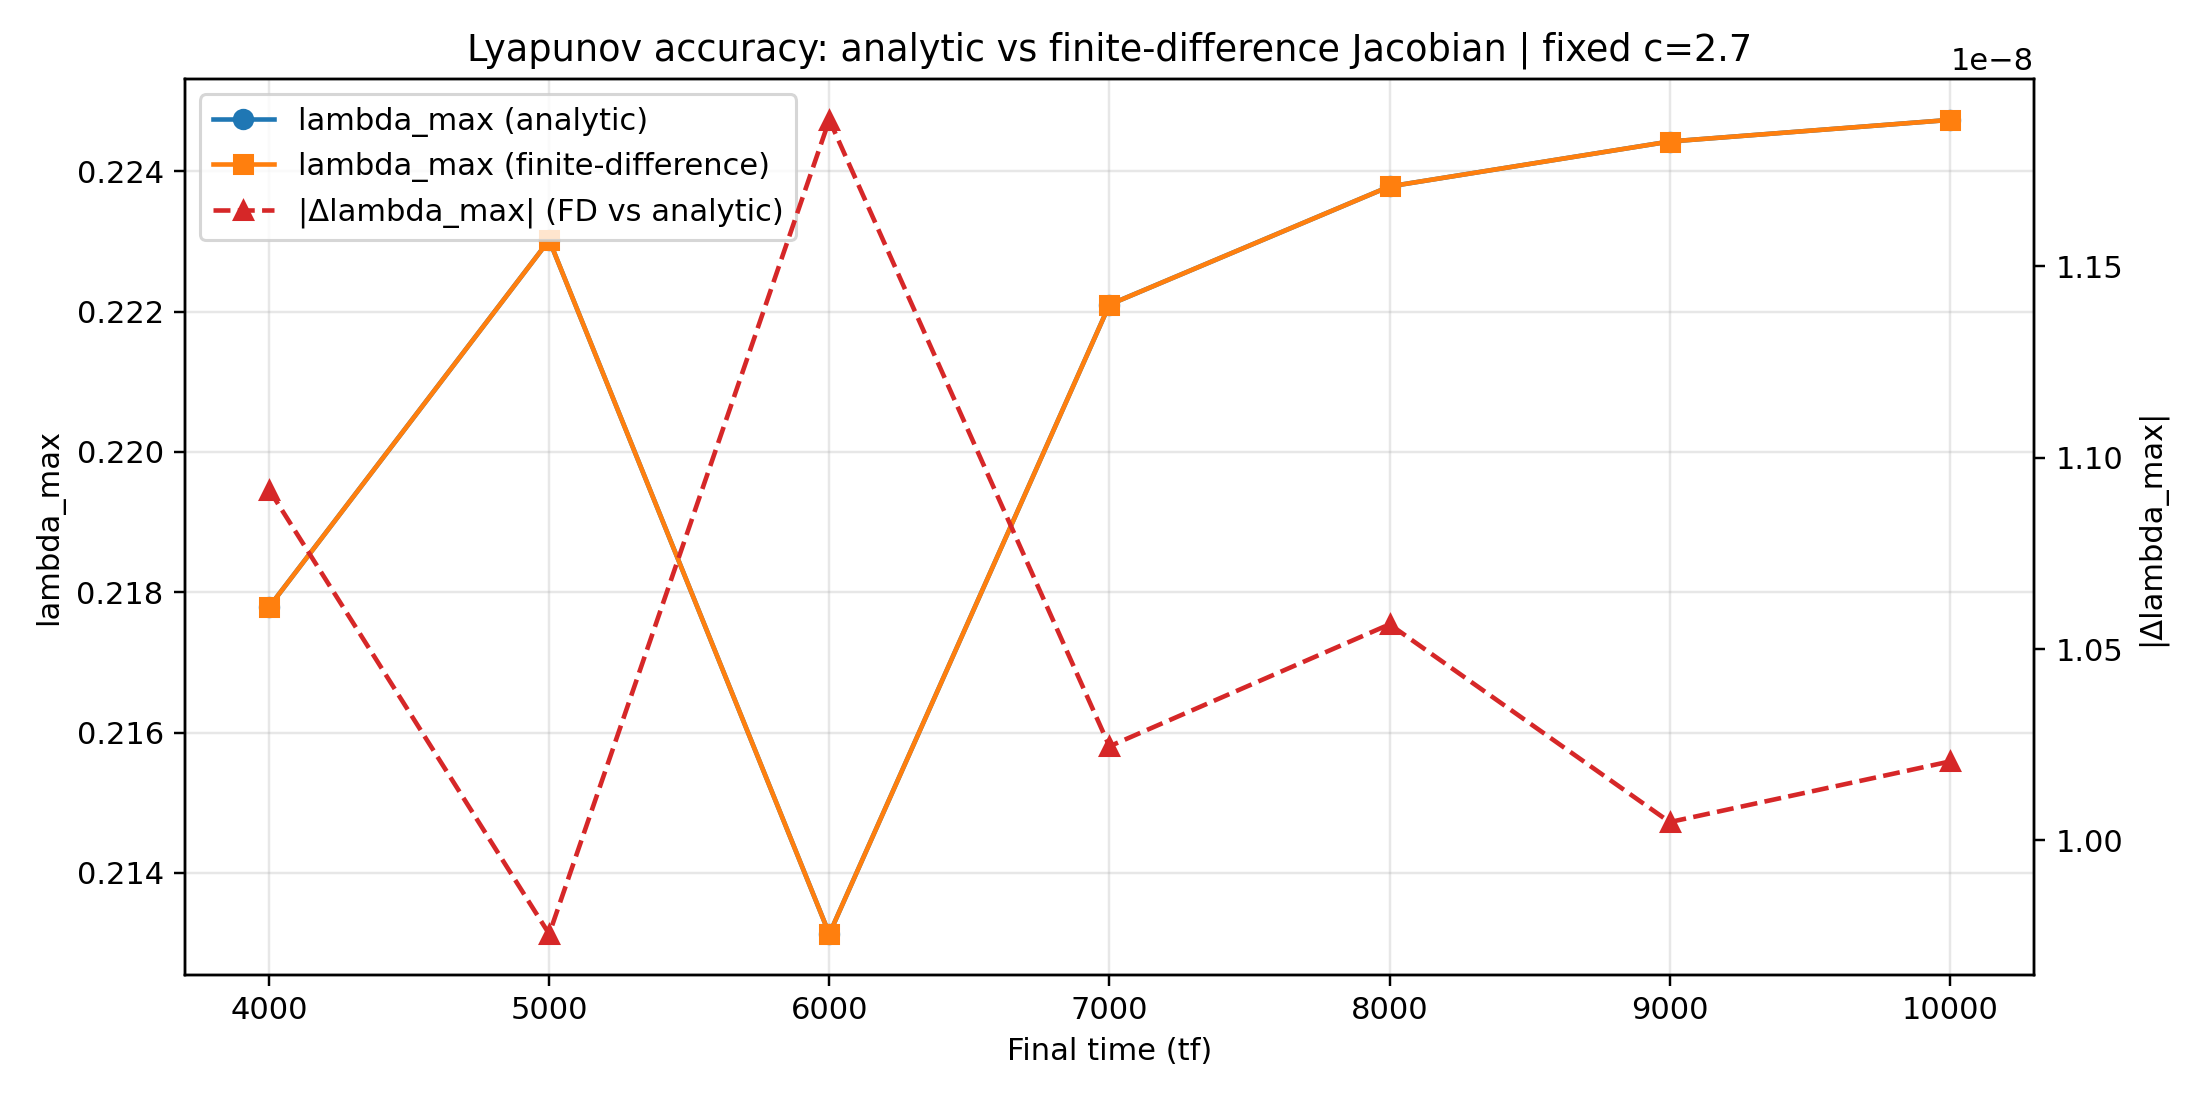
\includegraphics[width=\textwidth]{../../tests/lyapunov_benchmark_StaticParamsConfig_5_accuracy.png}
  \caption{Σύγκριση ακρίβειας (\(\lambda_{\max}\) analytic vs FD και \(|\Delta\lambda_{\max}|\))}
  \label{fig:ch2-lya-benchmark-accuracy}
\end{subfigure}
\hfill
\begin{subfigure}{0.48\textwidth}
  \centering
  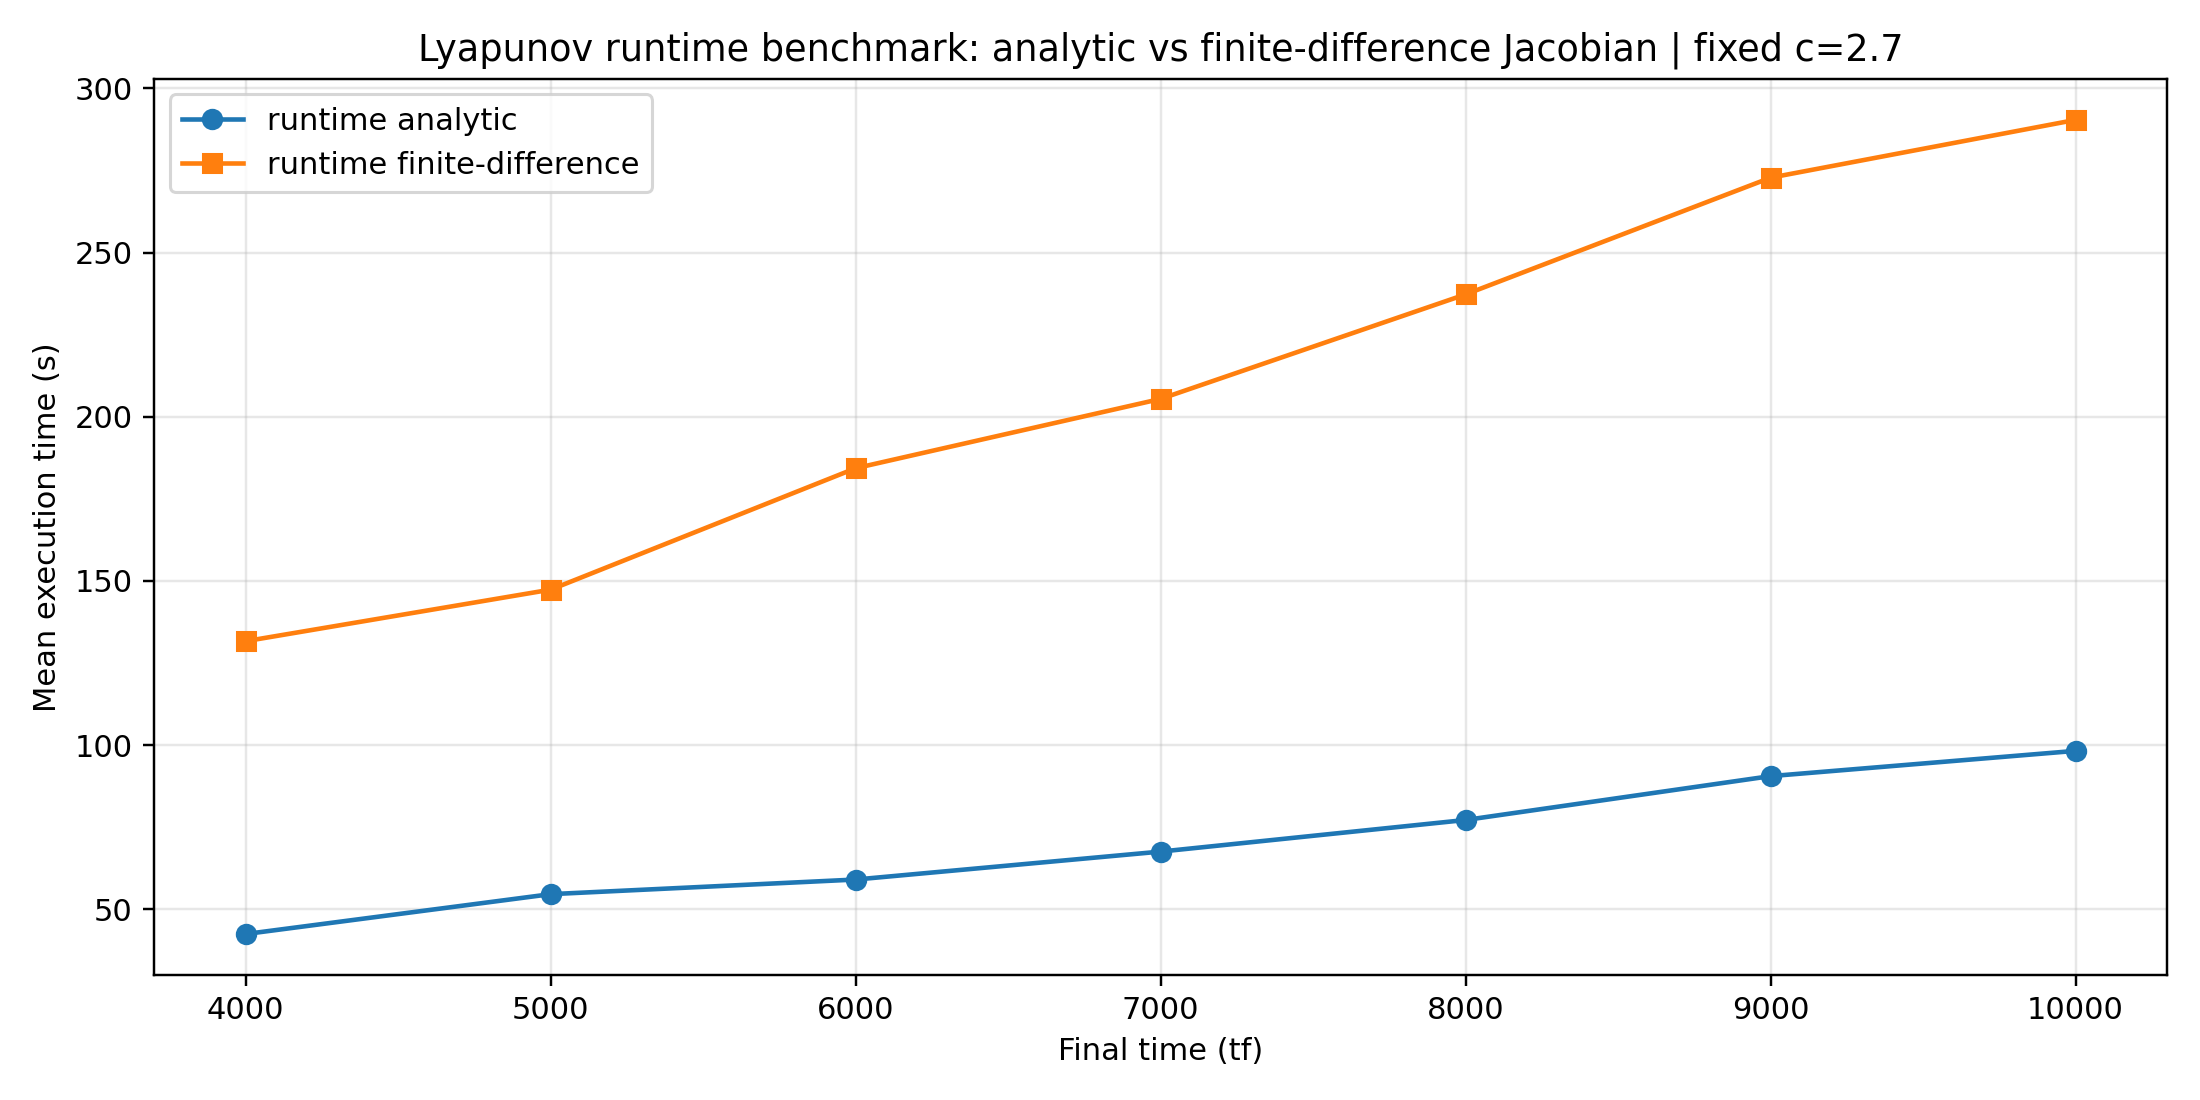
\includegraphics[width=\textwidth]{../../tests/lyapunov_benchmark_StaticParamsConfig_5_runtime.png}
  \caption{Σύγκριση χρόνου εκτέλεσης.}
  \label{fig:ch2-lya-benchmark-runtime}
\end{subfigure}
\caption{Benchmark Lyapunov Jacobian (analytic vs finite-difference) για \texttt{tests/StaticParamsConfig\_5.json}. Η ακρίβεια μεταξύ των δύο προσεγγίσεων συμπίπτει πρακτικά (αμελητέα, μη συστηματική απόκλιση), ενώ ο analytic Jacobian παρέχει αναμενόμενο speedup περίπου \(3\times\).}
\label{fig:ch2-lya-benchmark}
\end{figure}

\begin{resultsbox}
\paragraph{Συμπέρασμα benchmark.}
Για το συγκεκριμένο 4D παράδειγμα, δεν παρατηρείται ουσιαστική συστηματική απόκλιση στην
\(\lambda_{\max}\) μεταξύ analytic και finite-difference Jacobian (οι διαφορές είναι της τάξης
\(10^{-8}\)). Αντίθετα, στο runtime το όφελος είναι καθαρό: η διαδρομή με analytic Jacobian
εκτελείται περίπου τρεις φορές ταχύτερα, όπως αναμένεται από το χαμηλότερο υπολογιστικό
κόστος ανά βήμα.

Η παραπάνω πρακτική σύγκριση συνδέεται με τη γενικότερη χρήση lyapunov
δεικτών στη μελέτη σύνθετων μη γραμμικών δυναμικών συστημάτων,
το συγκεκριμένο παράδειγμα αντλήθηκε από \textit{Synchronization and anti-synchronization
of coupled hindmarsh-rose neuron models. Volos et al., 2016}.
\cite{volos2016_hindmarsh_sync}
\end{resultsbox}

\subsection{Parallel sweeps}

Για independent mode (χωρίς warm start), ιδανικά:
\begin{equation}
T_{\mathrm{wall}} \approx O\!\left(\frac{P}{W}\cdot \mathrm{cost\_per\_run}\right)
 + O(T_{\mathrm{overhead}}),
\end{equation}
όπου \(W\) ο αριθμός workers. Στο continuation mode δεν επιτρέπεται
παραλληλοποίηση λόγω αλυσιδωτής εξάρτησης αρχικών συνθηκών.

\section{Numba/JIT (just-in-time): interpreted έναντι compiled εκτέλεσης}
\label{sec:ch2-numba-jit}

\subsection{Ορισμοί}

\begin{toolbox}{Interpreted έναντι Compiled path στο έργο}{lam2015_numba,numba_jit_docs,numba_architecture_docs}
\textbf{Interpreted path:}
εκτέλεση Python bytecode από τον CPython interpreter
(UI (user interface), orchestration, fallbacks, adaptive \texttt{solve\_ivp} paths).

\textbf{Compiled path (Numba JIT (just-in-time)):}
μεταγλώττιση επιλεγμένων kernels σε machine code (μέσω \texttt{@njit}),
με εκτέλεση αριθμητικών βρόχων εκτός interpreter.
\end{toolbox}

\subsection{Πώς γίνεται η μεταγλώττιση μέσω Numba JIT (just-in-time)/LLVM (Low Level Virtual Machine)}

\begin{toolbox}{Pipeline μεταγλώττισης Numba JIT (just-in-time)/LLVM (Low Level Virtual Machine)}{lam2015_numba,numba_architecture_docs,numba_jit_docs,llvmlite_docs,llvm_langref}
Η Numba υλοποιεί \textit{just-in-time} μεταγλώττιση εξειδικευμένη στα πραγματικά
types των ορισμάτων που συναντά κατά την εκτέλεση. Η βασική ακολουθία
frontend/backend είναι η εξής:
\begin{enumerate}
\item \textbf{Ανάλυση Python συνάρτησης:} ο dispatcher της Numba ξεκινά από το
Python bytecode και χτίζει εσωτερική αναπαράσταση ροής ελέγχου (IR, intermediate representation / CFG (control-flow graph)).
\item \textbf{Type inference και specialization:} γίνεται επίλυση τύπων για μεταβλητές
και πράξεις. Όταν η επίλυση ολοκληρωθεί χωρίς Python objects, ενεργοποιείται
\texttt{nopython} path (το προτεινόμενο fast path).
\item \textbf{Lowering σε LLVM (Low Level Virtual Machine) IR (intermediate representation):} η typed Numba IR χαμηλώνεται σε LLVM IR μέσω
του \texttt{llvmlite}, που παρέχει το binding layer προς το LLVM (Low Level Virtual Machine) backend.
\item \textbf{Βελτιστοποίηση και παραγωγή native κώδικα:} εφαρμόζονται optimization
passes του LLVM (Low Level Virtual Machine) και παράγεται machine code για την τρέχουσα αρχιτεκτονική CPU (central processing unit).
\item \textbf{Caching και dispatch ανά signature:} ο compiled κώδικας αποθηκεύεται
ανά signature, ώστε επόμενες κλήσεις με ίδια signatures να αποφεύγουν το
κόστος επαναμεταγλώττισης.
\end{enumerate}
\end{toolbox}

Αν το \texttt{nopython} path δεν είναι εφικτό, η απόδοση συνήθως μειώνεται,
επειδή επανέρχονται μηχανισμοί του interpreter/object model. Για αυτό, στα
πειράματα της εργασίας χρησιμοποιούνται kernels σχεδιασμένοι για nopython
εκτέλεση \cite{numba_jit_docs,nlds_internal_scripts}.

Ακολουθεί το διάγραμμα ροής της μεταγλώττισης Numba JIT (just-in-time) προς LLVM (Low Level Virtual Machine) και native machine code.

\begin{figure}[H]
\centering
\includegraphics[width=0.96\textwidth]{figures/ch2/numba_jit_llvm_pipeline.png}
\caption{Σχηματική ροή μεταγλώττισης Numba JIT (just-in-time) προς LLVM (Low Level Virtual Machine) και native machine code,
με specialization ανά signature. Προσαρμοσμένο από την επίσημη τεκμηρίωση
Numba/llvmlite/LLVM (Low Level Virtual Machine) \cite{numba_architecture_docs,llvmlite_docs,llvm_langref}.}
\label{fig:ch2-numba-llvm-pipeline}
\end{figure}

\subsection{Πότε ενεργοποιείται Numba JIT (just-in-time)}

Η ενεργοποίηση ελέγχεται δυναμικά (\texttt{numba\_available()}):
\begin{itemize}
\item RK4 trajectories/sweeps: επιχειρείται Numba backend.
\item Symplectic Forest-Ruth: επιχειρείται Numba backend.
\item Lyapunov: Numba path κυρίως για \texttt{solver\_kind=rk4}.
\item RK45/DOP853 event-based sweeps: παραμένουν στην adaptive SciPy διαδρομή.
\end{itemize}

\subsection{Πότε εκτελείται compiled και πότε fallback}

Η πρακτική συμπεριφορά είναι:
\begin{enumerate}
\item \textbf{Πρώτη κλήση:} κόστος JIT (just-in-time) compilation.
\item \textbf{Επόμενες κλήσεις:} επαναχρησιμοποίηση compiled function
(σημαντικά μικρότερος χρόνος).
\item \textbf{Αν αποτύχει JIT (just-in-time) path} (μη διαθέσιμο Numba, ασυμβατό expression,
runtime exception στη δημιουργία kernel), ο controller κάνει fallback στην
Python υλοποίηση.
\end{enumerate}

\begin{importantbox}
Σημαντική τεχνική λεπτομέρεια:
\begin{itemize}
\item built-in Numba kernels: συνήθως \texttt{cache=True},
\item custom kernels (δυναμικό code generation): \texttt{cache=False}.
\end{itemize}

Άρα, το συνολικό runtime μοντέλο είναι \textit{υβριδικό}:
Python orchestration + επιλεγμένοι compiled αριθμητικοί πυρήνες.
\end{importantbox}

\subsection{Γιατί Numba αντί για εξωτερικό compiled backend (C/C++)}
\label{subsec:numba-vs-external-backend}

\begin{importantbox}
Στο συγκεκριμένο λογισμικό, η επιτάχυνση αφορά κυρίως τους ``θερμούς'' αριθμητικούς
βρόχους (RK4, Lyapunov, fixed-step sweeps), ενώ το υπόλοιπο workflow
παραμένει αναγκαστικά στον Python interpreter (UI (user interface) / Controller ροή, session state,
παραμετροποίηση, επιλογή solver, event/chunk orchestration, plotting/export).
Επομένως, ακόμη και με C/C++ numerical core, ο interpreter δεν αφαιρείται από
τη ροή εκτέλεσης.

Για αυτό το προφίλ workload, η επιλογή Numba υπερτερεί πρακτικά επειδή:
\begin{itemize}
\item \textbf{Αποφεύγεται το κόστος FFI (foreign function interface):} το FFI (foreign function interface) είναι η διεπαφή μέσω της οποίας
η Python καλεί κώδικα σε άλλη γλώσσα (π.χ. C/C++), και με εξωτερικό backend απαιτούνται
συνεχείς μεταβάσεις Python $\leftrightarrow$ native (marshaling, checks, ownership/shape συμφωνία πινάκων),
οι οποίες μπορεί να γίνουν συγκρίσιμες με το καθαρό αριθμητικό κόστος όταν οι κλήσεις είναι πολλές και σύντομες.
\item \textbf{Διατηρείται ενιαίο μοντέλο μνήμης NumPy:} οι JIT (just-in-time) kernels της Numba δουλεύουν in-process πάνω
σε ήδη υπάρχοντα arrays, χωρίς ξεχωριστό binding layer.
\item \textbf{Μειώνεται η πολυπλοκότητα συντήρησης:} ένας κώδικας Python με selective JIT (just-in-time) είναι ευκολότερος
στην εξέλιξη/δοκιμή/fallback σε σχέση με διπλό stack (Python + C/C++).
\item \textbf{Υπάρχει ομαλό fallback:} αν δεν είναι διαθέσιμη η Numba ή αποτύχει JIT (just-in-time) path, το σύστημα επιστρέφει
στην Python υλοποίηση χωρίς αλλαγή API (application programming interface).
\end{itemize}

Άρα, για υβριδικές εφαρμογές όπου η ορχήστρωση παραμένει σε Python, η Numba
δίνει συχνά καλύτερο \textit{end-to-end} tradeoff από έναν εξωτερικό compiled backend,
εκτός αν μεταφερθεί σε compiled γλώσσα και το μεγαλύτερο μέρος της
ορχήστρωσης (όχι μόνο οι kernels).
\end{importantbox}

\subsection{Σύγκριση backend επιλογών}
\label{subsec:backend-options-comparison}

\begin{guidebox}
Για αντικειμενικές συγκρίσεις Python vs Numba:
\begin{itemize}
\item απαιτείται warm-up πριν τις μετρήσεις,
\item πρέπει να αναφέρεται ρητά αν το Jacobian είναι analytic ή FD (finite difference),
\item χρειάζονται ίδιες τιμές \(dt\), \(t_{\mathrm{tr}}\), \(t_{\mathrm{m}}\), \(q\) (QR period, περίοδος ορθοκανονικοποίησης).
\end{itemize}
\end{guidebox}

\begin{resultsbox}
Τα αποτελέσματα του Πίνακα~\ref{tab:ch2-backend-runtime} προέρχονται από
εκτέλεση του script \texttt{tests/benchmark\_lyapunov\_cpp\_vs\_python.py}
(\texttt{Lorenz}, \texttt{solver=rk4}, analytic Jacobian,
\(dt=0.01\), \texttt{qr\_every\_steps}=10, \(t_{\mathrm{tr}}=500\),
sweep \(t_f=1000{:}1000{:}10000\), \texttt{runs}=3, \texttt{warmup}=1)
\cite{nlds_internal_scripts}.
\end{resultsbox}

\begin{table}[H]
\centering
\caption{Σύγκριση χρόνων εκτέλεσης backend για Lyapunov benchmark (ίδιο workload/ίδιες ρυθμίσεις).}
\label{tab:ch2-backend-runtime}
\renewcommand{\arraystretch}{1.15}
{\setlength{\tabcolsep}{4pt}
\begin{tabular}{|p{0.12\textwidth}|p{0.16\textwidth}|p{0.18\textwidth}|p{0.11\textwidth}|p{0.27\textwidth}|}
\hline
\textbf{Backend} & \textbf{Workload} & \textbf{Μέσος χρόνος (s)} & \textbf{Speedup vs Python} & \textbf{Παρατηρήσεις} \\
\hline
Python backend & Lorenz Lyapunov RK4 sweep & 35.3194 (εύρος: 6.7799-63.5325) & $1.00\times$ & Baseline interpreted path. \\
\hline
C++ backend & Lorenz Lyapunov RK4 sweep & 10.2832 (εύρος: 1.9980-18.4928) & $3.43\times$ & \texttt{nlds\_cpp} pybind11 backend από archived \texttt{cpp\_core}. \\
\hline
Numba backend & Lorenz Lyapunov RK4 sweep & 0.7260 (εύρος: 0.1462-1.3028) & $48.65\times$ & In-process JIT (just-in-time) nopython kernels σε NumPy arrays. \\
\hline
\end{tabular}
}
\end{table}

\begin{resultsbox}
Με βάση τις μετρήσεις του Πίνακα~\ref{tab:ch2-backend-runtime}, για ίδιο workload
ο Numba backend αποδίδει κατά μέσο όρο \(48.65\times\) ταχύτερα από το Python baseline,
ενώ ο C++ backend αποδίδει \(3.43\times\). Το αποτέλεσμα δείχνει ότι στο συγκεκριμένο
end-to-end προφίλ εκτέλεσης, το in-process JIT (just-in-time) path υπερέχει σαφώς.
\end{resultsbox}

\section{Αναπαραγωγιμότητα και διαχείριση πειραμάτων}

\begin{guidebox}
Η εφαρμογή υποστηρίζει:
\begin{itemize}
\item αποθήκευση στατικών configurations (Tab 1),
\item αποθήκευση sweep configurations (Tab 3),
\item session-state accumulation για continue workflows
(\texttt{sweep\_acc\_df}, \texttt{lya\_acc\_data}, fingerprints ρυθμίσεων).
\end{itemize}
\end{guidebox}

Η πρακτική αυτή μειώνει το πειραματικό drift και επιτρέπει ελεγχόμενη
επανάληψη αριθμητικών αποτελεσμάτων.


\section{Οδηγίες Υλοποίησης Προσομοίωσης}

Η ενότητα αυτή δίνει αναλυτικό, γενικό οδηγό εκτέλεσης μελέτης στο εργαλείο: από τον ορισμό του συστήματος μέχρι Lyapunov εκτίμηση, διαγράμματα διακλάδωσης και παραμετρικές σαρώσεις. Δεν εξαρτάται από συγκεκριμένο configuration αρχείο. Ένα έτοιμο config μπορεί να χρησιμοποιηθεί μόνο ως πρακτικό παράδειγμα εκκίνησης.

\subsection{Ελάχιστο σύνολο ρυθμίσεων πριν από κάθε run}

\begin{table}[H]
\centering
\caption{Ελάχιστο σύνολο ρυθμίσεων που πρέπει να οριστούν}
\label{tab:ch2-min-settings}
\renewcommand{\arraystretch}{1.15}
\begin{tabular}{|p{0.28\textwidth}|p{0.62\textwidth}|}
\hline
\textbf{Πεδίο} & \textbf{Περιγραφή / Τυπική επιλογή} \\
\hline
Μεταβλητές κατάστασης & Ονόματα κατάστασης ($x_1,\dots,x_n$) σύμφωνα με το μοντέλο. \\
\hline
Εξισώσεις & Μία εξίσωση ανά μεταβλητή, σε σύνταξη Python/SymPy. \\
\hline
Παράμετροι & Σταθερές μοντέλου με μορφή \texttt{name=value}. \\
\hline
Αρχική συνθήκη & $x_0 \in \mathbb{R}^n$, ίδια διάσταση με το σύστημα. \\
\hline
Ολοκλήρωση & $t_0, t_f, \Delta t$, solver kind (rk4/rk45/dop853/symplectic). \\
\hline
Lyapunov transient & $t_{\mathrm{tr}}$ ή \texttt{transient\_fraction}. \\
\hline
Lyapunov measure & $t_{\mathrm{m}}$: ενεργό παράθυρο συσσώρευσης $\log |R_{ii}|$. \\
\hline
QR ρύθμιση & \texttt{qr\_every\_steps=q} $\Rightarrow \Delta T_{\mathrm{QR}} = q\Delta t$. \\
\hline
Jacobian & \texttt{analytic} όταν είναι διαθέσιμος, αλλιώς finite-difference με \texttt{fd\_eps}. \\
\hline
\end{tabular}
\end{table}

\subsection{Σύνταξη εξισώσεων και υποστηριζόμενη γραφή}
\label{subsec:equation-syntax}

Οι custom εξισώσεις γράφονται σε σύνταξη Python/SymPy. Η μεταβλητή χρόνου \texttt{t} υποστηρίζεται για μη αυτόνομα συστήματα.

\begin{table}[H]
\centering
\caption{Τελεστές που χρησιμοποιούνται στη γραφή εξισώσεων}
\label{tab:ch2-operators}
\renewcommand{\arraystretch}{1.15}
\begin{tabular}{|p{0.30\textwidth}|p{0.18\textwidth}|p{0.40\textwidth}|}
\hline
\textbf{Περιγραφή} & \textbf{Σύνταξη} & \textbf{Παράδειγμα} \\
\hline
Πρόσθεση / αφαίρεση & \texttt{+}, \texttt{-} & \texttt{y - x} \\
\hline
Γινόμενο & \texttt{*} & \texttt{-x*z + u} \\
\hline
Διαίρεση & \texttt{/} & \texttt{(x + y)/2} \\
\hline
Ύψωση σε δύναμη & \texttt{**} & \texttt{x**2 + y**2} \\
\hline
Παρένθεση προτεραιότητας & \texttt{(...)} & \texttt{(x + y)*(z - u)} \\
\hline
Απόλυτη τιμή & \texttt{abs(...)} & \texttt{abs(x - y)} \\
\hline
\end{tabular}
\end{table}

\begin{table}[H]
\centering
\caption{Συναρτήσεις SymPy που χρησιμοποιούνται στη ροή custom parsing}
\label{tab:ch2-sympy-functions}
\renewcommand{\arraystretch}{1.15}
\begin{tabular}{|p{0.28\textwidth}|p{0.24\textwidth}|p{0.36\textwidth}|}
\hline
\textbf{Κατηγορία} & \textbf{Συνάρτηση} & \textbf{Παράδειγμα} \\
\hline
Τριγωνομετρικές & \texttt{sin, cos, tan} & \texttt{sin(x) + cos(y)} \\
\hline
Υπερβολικές & \texttt{sinh, cosh, tanh} & \texttt{tanh(z)} \\
\hline
Εκθετική / λογάριθμος & \texttt{exp, log} & \texttt{exp(-x) + log(1+x**2)} \\
\hline
Ρίζα / απόλυτη τιμή & \texttt{sqrt, abs} & \texttt{sqrt(x**2 + y**2)} \\
\hline
\end{tabular}
\end{table}

\subsubsection{Πρακτική σημείωση για \texttt{abs(...)} σε custom Jacobian}
\label{subsec:abs-custom-jacobian}

\begin{importantbox}
Η \texttt{abs(...)} υποστηρίζεται στο custom parsing, αλλά στο symbolic Jacobian
η SymPy (χωρίς ρητή υπόθεση ότι τα σύμβολα είναι πραγματικά) μπορεί να παράγει
όρους \texttt{re(...)}, \texttt{im(...)} και παραγώγους τύπου
\texttt{Derivative(re(y), y)}. Σε εξαγωγή NumPy κώδικα αυτό μπορεί να οδηγήσει
σε σφάλμα τύπου
\texttt{Unsupported by NumPyPrinter: Derivative}.
\end{importantbox}

\textbf{Παράδειγμα custom συστήματος:}
\begin{verbatim}
x' = -z
y' = x*z*z
z' = x - a*abs(y) + z*(b*y*y - z*z)
\end{verbatim}

\textbf{Ενδεικτικό symbolic Jacobian output (όπως εμφανίζεται στο preview):}
\begin{verbatim}
[0                               0                                  -1     ]
[                                                                          ]
[ 2                                                                        ]
[z                               0                                 2*x*z   ]
[                                                                          ]
[        /      d                 d        \                               ]
[      a*|re(y)*--(re(y)) + im(y)*--(im(y))|*sign(y)                       ]
[        \      dy                dy       /                       2      2]
[1   - --------------------------------------------- + 2*b*y*z  b*y  - 3*z ]
[                            y                                             ]
\end{verbatim}

\begin{guidebox}
\textbf{Ισοδύναμη real-only γραφή για \(\mathbf{y\in\mathbb{R}}\):}
\[
|y|=\sqrt{y^2}=y\,\operatorname{sign}(y)=
\begin{cases}
y, & y\ge 0\\
-y, & y<0
\end{cases}
\]
Άρα η τρίτη εξίσωση μπορεί να γραφτεί ισοδύναμα ως:
\[
z' = x - a\sqrt{y^2} + z\,(b y^2 - z^2)
\]
ή ως piecewise:
\[
z'=
\begin{cases}
x-a\,y+z\,(b y^2-z^2), & y\ge 0\\
x+a\,y+z\,(b y^2-z^2), & y<0
\end{cases}
\]
\end{guidebox}

\subsection{Βήμα-προς-βήμα ροή εκτέλεσης μελέτης}

\begin{guidebox}
\begin{enumerate}
\item \textbf{Ορισμός μοντέλου:} επιλέξτε built-in ή custom σύστημα, ορίστε μεταβλητές/εξισώσεις/παραμέτρους.
\item \textbf{Αρχικός αριθμητικός έλεγχος:} ορίστε προσωρινά μέτριο $t_f$ και σχετικά συντηρητικό $\Delta t$, εκτελέστε phase portrait και time-series για sanity check.
\item \textbf{Ρύθμιση solver:} επιλέξτε solver με βάση τον στόχο (Πίν.~\ref{tab:ch2-solver-choice}).
\item \textbf{Ρύθμιση Lyapunov:} ορίστε $t_{\mathrm{tr}}$, $t_{\mathrm{m}}$, $q$, επιλέξτε analytic Jacobian όπου υπάρχει.
\item \textbf{Βαθμονόμηση χρόνου και βήματος:} βρείτε $t_f$ και $\Delta t$ που σταθεροποιούν τους δείκτες χωρίς υπερβολικό runtime.
\item \textbf{Παραμετρική σάρωση:} αφού κλειδώσουν οι ρυθμίσεις single-run, προχωρήστε σε bifurcation/Lyapunov sweeps.
\item \textbf{Έλεγχος συνέπειας:} συγκρίνετε τα συμπεράσματα bifurcation και Lyapunov πριν οριστικοποιήσετε ερμηνεία.
\end{enumerate}
\end{guidebox}

\subsection{Επιλογή solver, transient και αριθμητικών ρυθμίσεων}

\begin{table}[H]
\centering
\caption{Κανόνες επιλογής solver ανά τύπο μελέτης}
\label{tab:ch2-solver-choice}
\renewcommand{\arraystretch}{1.15}
\begin{tabular}{|p{0.26\textwidth}|p{0.24\textwidth}|p{0.38\textwidth}|}
\hline
\textbf{Στόχος} & \textbf{Προτεινόμενος solver} & \textbf{Πρακτική οδηγία} \\
\hline
Γρήγορα Lyapunov runs & RK4 (fixed-step) & Συμβατό με Numba kernels, προβλέψιμο runtime, εύκολο benchmarking. \\
\hline
Baseline trajectory accuracy & RK45 / DOP853 & Χρήσιμο για cross-check τροχιών και event-based μελέτες. \\
\hline
Χαμιλτονιανά μακράς διάρκειας & Symplectic (Verlet/FR) & Προτιμάται για καλύτερη μακροχρόνια συμπεριφορά ενέργειας. \\
\hline
\end{tabular}
\end{table}

\begin{importantbox}
\textbf{Transient για Lyapunov:} επιλέξτε αρκετά μεγάλο $t_{\mathrm{tr}}$, ώστε η τροχιά να έχει ήδη εγκατασταθεί στον ελκυστή πριν ξεκινήσει η μέτρηση. Πρακτικά, ξεκινήστε από 30\% του συνολικού χρόνου και αυξήστε σε 40-60\% σε περιπτώσεις αργής μεταβατικής συμπεριφοράς.
\end{importantbox}

\subsection{Δύο πρακτικές επιλογές για σύγκλιση Lyapunov}

\begin{guidebox}
\textbf{Επιλογή 1 (incremental final-time test):}
\begin{enumerate}
\item Κρατήστε μικρό $\Delta t$ (π.χ. 0.01 ή μικρότερο).
\item Τρέξτε διαδοχικά $t_f = 5000, 10000, 15000$.
\item Συγκρίνετε τη μεταβολή του $\lambda_{\max}$ μεταξύ διαδοχικών runs.
\item Όταν η τιμή σταθεροποιείται στα δεκαδικά που σας ενδιαφέρουν, θεωρήστε ότι έχετε επαρκές $t_f$ για τη συγκεκριμένη μελέτη.
\item Για παραμετρικές σαρώσεις Lyapunov γυρίστε σε πιο ``χαλαρή'' ακρίβεια (λίγο μεγαλύτερο $\Delta t$ ή/και μικρότερο $t_f$), διατηρώντας όμως το ίδιο ποιοτικό καθεστώς.
\end{enumerate}
\end{guidebox}

\begin{guidebox}
\textbf{Επιλογή 2 (notebook-based plateau detection):}
\begin{enumerate}
\item Τρέξτε notebook ανάλυσης (π.χ. \texttt{examples/dynSystemSim.ipynb}) ώστε να παραχθεί καμπύλη $\lambda_{\max}(t)$ ή $\lambda_{\max}$ vs $t_f$.
\item Εντοπίστε οπτικά πού ξεκινά το ασυμπτωτικό πλατώ.
\item Επιλέξτε $t_f$ στο πλατώ με ένα εύλογο περιθώριο ασφαλείας.
\item Χρησιμοποιήστε αυτό το $t_f$ ως baseline για την παραμετρική σάρωση.
\end{enumerate}
\end{guidebox}

\begin{importantbox}
\textbf{Κανόνας για $\Delta t$:} αυξάνετε προοδευτικά το time step μέχρι να εμφανιστεί αισθητή αλλοίωση στα αποτελέσματα (Lyapunov, γεωμετρία ελκυστή, Poincar\'e σημεία). Επιλέγετε τελικά το μέγιστο $\Delta t$ λίγο πριν την αλλοίωση.

\textbf{Πρακτική ακρίβειας Lyapunov:} οι εκθέτες Lyapunov είναι κυρίως ποιοτικοί δείκτες δυναμικής συμπεριφοράς (χάος/περιοδικότητα/σταθερότητα). Συνήθως δεν απαιτείται υπερβολική αριθμητική ακρίβεια πέρα από το σημείο όπου η ποιοτική ταξινόμηση δεν αλλάζει.
\end{importantbox}

\subsection{Κρίσιμος έλεγχος: συνέπεια διαγράμματος διακλάδωσης και Lyapunov}

\begin{resultsbox}
\textbf{Κανόνας ερμηνείας σε παραμετρική σάρωση:} η συμπεριφορά του διαγράμματος διακλάδωσης πρέπει να συμφωνεί με τις αντίστοιχες Lyapunov τιμές.
\begin{itemize}
\item Περιοδικά παράθυρα $\Rightarrow \lambda_{\max} \le 0$ (ή πολύ κοντά στο 0 εντός ανοχής).
\item Χαοτικές περιοχές $\Rightarrow \lambda_{\max} > 0$.
\item Μεταβάσεις/οριακές περιοχές $\Rightarrow$ έλεγχος με finer grid ή λίγο μικρότερο $\Delta t$.
\end{itemize}
Αν η αντιστοίχιση δεν είναι συνεπής, η σάρωση δεν θεωρείται ακόμη αριθμητικά ώριμη και απαιτεί νέα βαθμονόμηση ($t_f$, $\Delta t$, $t_{\mathrm{tr}}$, $q$).
\end{resultsbox}

\subsection{Παραλληλοποίηση: πότε ναι και πότε όχι}

\begin{table}[H]
\centering
\caption{Κανόνες παραλληλοποίησης σε sweeps}
\label{tab:ch2-parallel-rules}
\renewcommand{\arraystretch}{1.15}
\begin{tabular}{|p{0.34\textwidth}|p{0.16\textwidth}|p{0.36\textwidth}|}
\hline
\textbf{Τύπος sweep} & \textbf{Parallel} & \textbf{Αιτιολόγηση} \\
\hline
Bifurcation mode (reset ICs) & Ναι & Κάθε τιμή παραμέτρου είναι ανεξάρτητο run. \\
\hline
Continuation mode (warm start) & Όχι & Υπάρχει αλυσιδωτή εξάρτηση αρχικών συνθηκών. \\
\hline
Lyapunov parameter sweep & Ναι & Ανεξάρτητες εκτιμήσεις ανά τιμή παραμέτρου. \\
\hline
\end{tabular}
\end{table}

\begin{guidebox}
\textbf{Πρακτική σύσταση:}
\begin{enumerate}
\item Σε bifurcation (reset) και Lyapunov sweeps ενεργοποιήστε parallel workers.
\item Σε continuation κρατήστε σειριακή εκτέλεση.
\item Σε μεγάλα sweeps ξεκινήστε με μικρότερο πλήθος παραμέτρων για sanity check και μετά αυξήστε την ανάλυση.
\end{enumerate}
\end{guidebox}


\chapter{Υλοποιήσεις - Παραδείγματα}
\label{ch:implementations-examples}

\noindent\textbf{Chapter summary.}
\textenglish{This chapter presents a structured reproduction workflow for representative results reported in three nonlinear-dynamics papers. For each case study, the objective is to recreate the main qualitative signatures (attractor morphology, periodic/chaotic regimes) under a transparent and repeatable numerical protocol. The chapter standardizes the reproduction sequence: model transcription, parameter/initial-condition alignment, solver and time-window calibration, baseline validation, and side-by-side comparison between literature and simulator outputs. It also defines placeholders for comparative figures and summary tables so that final manuscript integration can be completed without redesigning the chapter structure when the final plots are exported.}

\section{Πλαίσιο Αναπαραγωγής Αποτελεσμάτων}

Το κεφάλαιο αυτό συγκεντρώνει την πρακτική αναπαραγωγή αποτελεσμάτων από τρία ενδεικτικά papers μη γραμμικής δυναμικής, με στόχο:
\begin{itemize}
\item ποιοτική συμφωνία (τύπος ελκυστή, περιοδικότητα/χάος),
\item ποσοτική σύγκριση βασικών δεικτών όπου αυτό είναι εφικτό,
\item ενιαία παρουσίαση συγκριτικών διαγραμμάτων για το τελικό report.
\end{itemize}

\begin{guidebox}
\textbf{Ενιαίο πρωτόκολλο αναπαραγωγής}
\begin{enumerate}
\item Καταγραφή μοντέλου, παραμέτρων και αρχικών συνθηκών από το paper.
\item Ευθυγράμμιση solver settings ($\Delta t$, $t_f$, transient, tolerances).
\item Εκτέλεση baseline run για έλεγχο μορφολογίας τροχιάς/ελκυστή.
\item Παραγωγή αντίστοιχων διαγραμμάτων (phase, time series, Poincar\'e, Lyapunov).
\item Τοποθέτηση side-by-side συγκρίσεων: Paper vs Αναπαραγωγή.
\end{enumerate}
\end{guidebox}

\section{Paper 1: No-Equilibrium Chaotic System}

Αναπαραγωγή με βάση το \cite{pham2014_no_equilibrium}.

\subsection{Στόχος Αναπαραγωγής}

Στόχος είναι η επιβεβαίωση της ποιοτικής δομής του ελκυστή και της δυναμικής συμπεριφοράς που αναφέρεται στο paper, με ισοδύναμη παραμετροποίηση στο εργαλείο.

\subsection{Placeholders Συγκριτικών Διαγραμμάτων}

Στο παρακάτω σχήμα τοποθετούνται τα τρία placeholders σύγκρισης για το Paper 1.

\begin{figure}[H]
\centering
\begin{subfigure}[t]{0.31\textwidth}
\centering
\fbox{\parbox[c][4.2cm][c]{0.95\linewidth}{\centering Placeholder\\Paper 1\\(δημοσιευμένο διάγραμμα)}}
\end{subfigure}
\hfill
\begin{subfigure}[t]{0.31\textwidth}
\centering
\fbox{\parbox[c][4.2cm][c]{0.95\linewidth}{\centering Placeholder\\Paper 1\\(αναπαραγωγή στο εργαλείο)}}
\end{subfigure}
\hfill
\begin{subfigure}[t]{0.31\textwidth}
\centering
\fbox{\parbox[c][4.2cm][c]{0.95\linewidth}{\centering Placeholder\\Paper 1\\(συγκριτική απεικόνιση)}}
\end{subfigure}
\caption{Paper 1: θέση για σύγκριση βιβλιογραφικού αποτελέσματος και αναπαραγωγής.}
\label{fig:ch3-paper1-placeholder}
\end{figure}

\section{Paper 2: Rounded-Square Chaotic Attractor}

Αναπαραγωγή με βάση το \cite{pham2017_rounded_square}.

\subsection{Στόχος Αναπαραγωγής}

Στόχος είναι η επαλήθευση της χαρακτηριστικής γεωμετρίας του ελκυστή και η αντιστοίχιση των βασικών ποιοτικών περιοχών δυναμικής.

\subsection{Placeholders Συγκριτικών Διαγραμμάτων}

Στο παρακάτω σχήμα τοποθετούνται τα τρία placeholders σύγκρισης για το Paper 2.

\begin{figure}[H]
\centering
\begin{subfigure}[t]{0.31\textwidth}
\centering
\fbox{\parbox[c][4.2cm][c]{0.95\linewidth}{\centering Placeholder\\Paper 2\\(δημοσιευμένο διάγραμμα)}}
\end{subfigure}
\hfill
\begin{subfigure}[t]{0.31\textwidth}
\centering
\fbox{\parbox[c][4.2cm][c]{0.95\linewidth}{\centering Placeholder\\Paper 2\\(αναπαραγωγή στο εργαλείο)}}
\end{subfigure}
\hfill
\begin{subfigure}[t]{0.31\textwidth}
\centering
\fbox{\parbox[c][4.2cm][c]{0.95\linewidth}{\centering Placeholder\\Paper 2\\(συγκριτική απεικόνιση)}}
\end{subfigure}
\caption{Paper 2: θέση για σύγκριση βιβλιογραφικού αποτελέσματος και αναπαραγωγής.}
\label{fig:ch3-paper2-placeholder}
\end{figure}

\section{Paper 3: Four-Wing Memristive Chaotic System}

Αναπαραγωγή με βάση το \cite{pham2016_hyperjerk_memristive}.

\subsection{Στόχος Αναπαραγωγής}

Στόχος είναι η αναπαραγωγή του τύπου ελκυστή και των αντίστοιχων υπογραφών χάους μέσω phase portraits και συνοδευτικών μετρικών.

\subsection{Placeholders Συγκριτικών Διαγραμμάτων}

Στο παρακάτω σχήμα τοποθετούνται τα τρία placeholders σύγκρισης για το Paper 3.

\begin{figure}[H]
\centering
\begin{subfigure}[t]{0.31\textwidth}
\centering
\fbox{\parbox[c][4.2cm][c]{0.95\linewidth}{\centering Placeholder\\Paper 3\\(δημοσιευμένο διάγραμμα)}}
\end{subfigure}
\hfill
\begin{subfigure}[t]{0.31\textwidth}
\centering
\fbox{\parbox[c][4.2cm][c]{0.95\linewidth}{\centering Placeholder\\Paper 3\\(αναπαραγωγή στο εργαλείο)}}
\end{subfigure}
\hfill
\begin{subfigure}[t]{0.31\textwidth}
\centering
\fbox{\parbox[c][4.2cm][c]{0.95\linewidth}{\centering Placeholder\\Paper 3\\(συγκριτική απεικόνιση)}}
\end{subfigure}
\caption{Paper 3: θέση για σύγκριση βιβλιογραφικού αποτελέσματος και αναπαραγωγής.}
\label{fig:ch3-paper3-placeholder}
\end{figure}

\section{Συγκεντρωτικά Συγκριτικά Διαγράμματα}

Ακολουθούν τα συγκεντρωτικά placeholders για τη συνολική σύγκριση των τριών αναπαραγωγών.

\begin{figure}[H]
\centering
\begin{subfigure}[t]{0.48\textwidth}
\centering
\fbox{\parbox[c][4.3cm][c]{0.95\linewidth}{\centering Placeholder\\Συγκεντρωτικό phase-portrait comparison\\(3 papers)}}
\end{subfigure}
\hfill
\begin{subfigure}[t]{0.48\textwidth}
\centering
\fbox{\parbox[c][4.3cm][c]{0.95\linewidth}{\centering Placeholder\\Συγκεντρωτικό Lyapunov / δείκτες\\(3 papers)}}
\end{subfigure}
\caption{Συγκεντρωτικά συγκριτικά διαγράμματα για τις τρεις αναπαραγωγές.}
\label{fig:ch3-summary-placeholders}
\end{figure}

\begin{table}[H]
\centering
\caption{Placeholder πίνακας σύνοψης αναπαραγωγής για τα 3 papers}
\label{tab:ch3-reproduction-summary}
\renewcommand{\arraystretch}{1.2}
\begin{tabular}{|l|l|l|p{0.3\textwidth}|}
\hline
\textbf{Paper} & \textbf{Δείκτης paper} & \textbf{Δείκτης αναπαραγωγής} & \textbf{Παρατήρηση} \\
\hline
\cite{pham2014_no_equilibrium} & Placeholder & Placeholder & Placeholder σχολιασμού \\
\hline
\cite{pham2017_rounded_square} & Placeholder & Placeholder & Placeholder σχολιασμού \\
\hline
\cite{pham2016_hyperjerk_memristive} & Placeholder & Placeholder & Placeholder σχολιασμού \\
\hline
\end{tabular}
\end{table}

\chapter{Σύνοψη - Ανοιχτά Θέματα}
\label{ch:summary-open-topics}

\noindent\textbf{Chapter summary.}
\textenglish{This chapter synthesizes the contributions of the thesis and frames the main open research and engineering directions. It consolidates what has been achieved at methodological, software-architecture, and experimental-validation levels, and it outlines concrete next steps for research-grade maturation of the platform.}

\section{Τι προσφέρει η εργασία}

\begin{itemize}
\item Εργαλείο με ανεξάρτητο backend για επαναχρησιμοποίηση: ο αριθμητικός πυρήνας είναι διαχωρισμένος από τη διεπαφή και μπορεί να τροφοδοτήσει νέες ερευνητικές εργασίες είτε μέσω Python/Numba kernels είτε μέσω external C++ backend, ανάλογα με τις ανάγκες του workflow.
\item Python frontend (Streamlit) ως template: η αρχιτεκτονική της εφαρμογής λειτουργεί ως πρότυπο για scientific computing / computational physics projects από developers χωρίς εξειδικευμένη εμπειρία frontend, με καθαρό διαχωρισμό UI (user interface)-Controller-Core.
\item Χρήση χωρίς ανάγκη εκτεταμένης γραφής κώδικα: ο βασικός κύκλος πειραμάτων (ρύθμιση, εκτέλεση, οπτικοποίηση, αποθήκευση configuration) παραμένει διαθέσιμος μέσω UI (user interface).
\item Εστιασμένες λειτουργίες για μη γραμμικά δυναμικά συστήματα: phase portraits, Poincar\'e sections, bifurcation sweeps και Lyapunov εκτίμηση.
\item Αναπαραγωγιμότητα και πειραματική πειθαρχία: υποστηρίζονται αποθήκευση ρυθμίσεων, accumulation state για continuation workflows και τυποποιημένα benchmark scripts.
\end{itemize}

\section{Ανοιχτά Θέματα}

\begin{itemize}
\item Τοπική ή cloud διάθεση (Docker): πακετοποίηση του εργαλείου ως local/cloud υπηρεσία με έμφαση σε παραγωγή συγκριτικών διαγραμμάτων και ροών ανάλυσης.
\item Εμπλουτισμός βιβλιοθήκης solvers: προσθήκη περισσότερων μεθόδων για ευρύτερη κάλυψη προβλημάτων (π.χ. Radau/implicit επιλογές, DDE (delay differential equations) solvers, εξειδικευμένα stiff workflows).
\item Αυτόματη προτεινόμενη παραμετροποίηση: μηχανισμός αυτόματης διερεύνησης που θα προτείνει αρχικές τιμές για $t_f$, $\Delta t$, transient window και κρίσιμα παραμετρικά ranges.
\item Ενσωματωμένοι δείκτες αξιοπιστίας: αυτόματοι έλεγχοι σύγκλισης/σταθερότητας (step-size sensitivity, tolerance sweeps, finite-time variance checks).
\item Τυποποιημένη εξαγωγή ερευνητικών reports: αυτόματη παραγωγή artifact bundle (figures, tables, metadata, configs, run hashes) για άμεση τεκμηρίωση και αναπαραγωγή.
\end{itemize}


% ============================================================
\appendix
% ============================================================

\chapter*{Παράρτημα Κεφαλαίου 1}
\addcontentsline{toc}{chapter}{Παράρτημα Κεφαλαίου 1}
\setcounter{section}{0}
\newcommand{\appendixletter}[1]{%
  \ifcase#1%
  \or A\or B\or C\or D\or E\or F\or G\or H\or I\or J%
  \else #1%
  \fi%
}
\renewcommand{\thesection}{\appendixletter{\value{section}}}
\renewcommand{\thesubsection}{\thesection.\arabic{subsection}}

\section{Σύνοψη διεπαφής και συμβάσεων δεδομένων του \texttt{solver.py}}
\label{app:solver-interface}
\begin{importantbox}
Ο \texttt{solver.py} ορίζει ένα ελαφρύ δοχείο αποτελέσματος (\texttt{OdeSolution}) και δύο ολοκληρωτές:
\begin{itemize}
  \item \texttt{integrate\_system}: επίλυση IVP (initial value problem) μέσω \texttt{scipy.integrate.solve\_ivp} και επιστροφή δειγματοληπτημένων τιμών σε \texttt{t\_eval}.
  \item \texttt{integrate\_system\_rk4}: σταθερού βήματος κλασικό RK4 για ελεγχόμενη/αναπαραγώγιμη σύγκριση.
\end{itemize}
Η έξοδος έχει τη μορφή:
\begin{equation*}
t \in \mathbb{R}^{N}, \qquad y \in \mathbb{R}^{d \times N},
\end{equation*}
ώστε μια προβολή φασικού διαγράμματος $y_i$-$y_j$ να υλοποιείται άμεσα ως ζεύγη $(y_i(t_k),y_j(t_k))$ για $k=1,\dots,N$.
\end{importantbox}

\subsection*{Ψευδοκώδικας: Ολοκλήρωση τροχιάς για φασικά διαγράμματα}
\begin{algorithm}[H]
\caption{Trajectory integration for phase portraits}
\label{alg:traj-phase}
\begin{tcolorbox}[appendixalgobox]
\begin{algorithmic}[1]
\Require $f(t,\mathbf{x})$, $[t_0,t_f]$, $\mathbf{x}_0$, $\Delta t$
\Ensure Arrays $\{t_k\}$ and $\{\mathbf{x}(t_k)\}$
\State Construct evaluation grid $t_k = t_0 + k\Delta t$
\State Solve IVP (initial value problem) to obtain $\mathbf{x}(t_k)$
\State Return arrays $\{t_k\}$ and $\{\mathbf{x}(t_k)\}$
\end{algorithmic}
\end{tcolorbox}
\end{algorithm}

\subsection*{Ψευδοκώδικας: Fixed-step RK4 (όπως στο \texttt{core/solver.py})}
\begin{algorithm}[H]
\caption{\texttt{integrate\_system\_rk4}}
\label{alg:rk4-fixed}
\begin{tcolorbox}[appendixalgobox]
\begin{algorithmic}[1]
\Require RHS (right-hand side) $f(t,\mathbf{y})$, $[t_0,t_f]$, $\mathbf{y}_0$, step $h$, optional \texttt{max\_steps}
\Ensure \texttt{OdeSolution} with time grid and state history
\State $\mathbf{y}_0 \gets \texttt{np.array}(\mathbf{y}_0,\texttt{dtype=float})$
\State $N \gets \texttt{\_compute\_n\_steps}(t_0,t_f,h,\texttt{max\_steps})$
\State $d \gets \dim(\mathbf{y}_0)$
\State Allocate $t \in \mathbb{R}^{N}$ and $Y \in \mathbb{R}^{d\times N}$ with zeros
\State $t[0]\gets t_0,\; Y[:,0]\gets \mathbf{y}_0$
\For{$i=1,\dots,N-1$}
  \State $t_i \gets t[i-1],\; \mathbf{y}_i \gets Y[:,i-1]$
  \If{$t_i \ge t_f$}
    \State $t \gets t[:i],\; Y \gets Y[:,:i]$
    \State \textbf{break}
  \EndIf
  \State $\mathbf{k}_1 \gets f(t_i,\mathbf{y}_i)$
  \State $\mathbf{k}_2 \gets f(t_i+\tfrac{h}{2},\mathbf{y}_i+\tfrac{h}{2}\mathbf{k}_1)$
  \State $\mathbf{k}_3 \gets f(t_i+\tfrac{h}{2},\mathbf{y}_i+\tfrac{h}{2}\mathbf{k}_2)$
  \State $\mathbf{k}_4 \gets f(t_i+h,\mathbf{y}_i+h\mathbf{k}_3)$
  \State $Y[:,i] \gets \mathbf{y}_i + \tfrac{h}{6}\left(\mathbf{k}_1 + 2\mathbf{k}_2 + 2\mathbf{k}_3 + \mathbf{k}_4\right)$
  \State $t[i] \gets t_i + h$
\EndFor
\State \Return \texttt{OdeSolution}(t,Y,\texttt{success=True},\texttt{message="RK4 integration completed."})
\end{algorithmic}
\end{tcolorbox}
\end{algorithm}

\subsection*{Ψευδοκώδικας: Symplectic Forest-Ruth 4ης τάξης (όπως στο \texttt{core/symplectic\_solver.py})}
\begin{algorithm}[H]
\caption{\texttt{integrate\_system\_symplectic\_fr}}
\label{alg:fr4}
\begin{tcolorbox}[appendixalgobox]
\begin{algorithmic}[1]
\Require Separable Hamiltonian state $\mathbf{z}=[\mathbf{q},\mathbf{p}]$, $[t_0,t_f]$, $\mathbf{z}_0$, step $h$, optional \texttt{max\_steps}, \texttt{dp\_dt}, optional \texttt{dq\_dt}
\Ensure \texttt{OdeSolution} preserving symplectic update structure
\State Convert $\mathbf{z}_0$ to 1D float array and set $n_q \gets \texttt{options.get("n\_q", len(}\mathbf{z}_0\texttt{)//2)}$
\State Validate $\dim(\mathbf{z}_0)=2n_q$ and \texttt{dp\_dt} callable
\If{\texttt{dq\_dt} not provided}
  \State Set $\texttt{dq\_dt}(t,\mathbf{p})=\mathbf{p}$
\EndIf
\State $N \gets \texttt{\_compute\_n\_steps}(t_0,t_f,h,\texttt{max\_steps})$
\State $t \gets \texttt{linspace}(t_0,t_f,N)$,\; allocate $Y \in \mathbb{R}^{2n_q\times N}$ with zeros,\; $Y[:,0]\gets \mathbf{z}_0$
\State $w \gets \dfrac{1}{2-2^{1/3}},\; c_1\gets w,\; c_2\gets 1-2w,\; c_3\gets w$
\Statex
\State \textbf{Auxiliary step} $\texttt{VerletStep}(t,\mathbf{q},\mathbf{p},\Delta h)$:
\State \hspace{1em}$\mathbf{p}_{1/2} \gets \mathbf{p} + \tfrac{1}{2}\Delta h\;\texttt{dp\_dt}(t,\mathbf{q})$
\State \hspace{1em}$\mathbf{q}_{\text{new}} \gets \mathbf{q} + \Delta h\;\texttt{dq\_dt}(t,\mathbf{p}_{1/2})$
\State \hspace{1em}$\mathbf{p}_{\text{new}} \gets \mathbf{p}_{1/2} + \tfrac{1}{2}\Delta h\;\texttt{dp\_dt}(t+\Delta h,\mathbf{q}_{\text{new}})$
\State \hspace{1em}\Return $(t+\Delta h,\mathbf{q}_{\text{new}},\mathbf{p}_{\text{new}})$
\Statex
\For{$i=1,\dots,N-1$}
  \State $t_i \gets t[i-1]$, split $Y[:,i-1]$ into $(\mathbf{q},\mathbf{p})$
  \State $(t_i,\mathbf{q},\mathbf{p}) \gets \texttt{VerletStep}(t_i,\mathbf{q},\mathbf{p},c_1h)$
  \State $(t_i,\mathbf{q},\mathbf{p}) \gets \texttt{VerletStep}(t_i,\mathbf{q},\mathbf{p},c_2h)$
  \State $(t_i,\mathbf{q},\mathbf{p}) \gets \texttt{VerletStep}(t_i,\mathbf{q},\mathbf{p},c_3h)$
  \State $Y[:,i] \gets [\mathbf{q};\mathbf{p}]$
\EndFor
\State \Return \texttt{OdeSolution}(t,Y,\texttt{success=True},\texttt{message="Symplectic Forest-Ruth (FR) integration completed."})
\end{algorithmic}
\end{tcolorbox}
\end{algorithm}


\section{Επιλογές δειγματοληψίας και αναπαραγωγιμότητα}
\label{app:sampling}
Ο αριθμός σημείων δειγματοληψίας καθορίζεται από \texttt{t\_step} (ή ισοδύναμα από \texttt{max\_steps}) και κατασκευάζεται \texttt{t\_eval} ως ισαπέχον πλέγμα στο $[t_0,t_f]$.
Αυτό διασφαλίζει σταθερή χρονική βάση για τα γραφήματα (time series και phase portraits) και επιτρέπει συνεπή σύγκριση μεταξύ διαφορετικών εκτελέσεων/παραμέτρων, υπό την προϋπόθεση ότι οι ανοχές και το χρονικό διάστημα παραμένουν ίδια.

\section{Έλεγχοι ορθότητας εισόδων και ασφαλείς προεπιλογές}
\label{app:input-checks}
Ο κώδικας περιλαμβάνει ελέγχους βασικής εγκυρότητας (π.χ.\ \texttt{t\_step > 0}) και ενιαία μετατροπή της αρχικής συνθήκης σε διάνυσμα \texttt{float}, ώστε η αριθμητική ροή να είναι συνεπής.
Η ύπαρξη μηνύματος/σημαίας επιτυχίας (\texttt{success}, \texttt{message}) επιτρέπει στο περιβάλλον χρήστη να εντοπίζει αποτυχίες ολοκλήρωσης και να αποφεύγει την παραγωγή παραπλανητικών διαγραμμάτων.

\subsection*{Πίνακας μηνυμάτων διεπαφής και αντιμετώπισης}
\label{app:ui-messages}
Ο Πίνακας~\ref{tab:ui-messages-troubleshooting} συνοψίζει τα συχνότερα μηνύματα
σφάλματος/προειδοποίησης/διάγνωσης που εμφανίζονται στη διεπαφή και
προτείνει πρακτικά βήματα επίλυσης.

\begin{table}[H]
\centering
\caption{Συνοπτικός οδηγός ερμηνείας μηνυμάτων UI}
\label{tab:ui-messages-troubleshooting}
\renewcommand{\arraystretch}{1.2}
\small
\begin{tabular}{|p{0.36\textwidth}|p{0.27\textwidth}|p{0.29\textwidth}|}
\hline
\textbf{Μήνυμα (UI)} & \textbf{Τι σημαίνει} & \textbf{Προτεινόμενη αντιμετώπιση} \\
\hline
\texttt{Coverage: observed/expected parameter values have hits ...} &
Δεν προέκυψαν τομές Poincaré (hits) για όλες τις τιμές της παραμέτρου στο επιλεγμένο sweep εύρος. &
Μειώστε \texttt{dt} (π.χ.\ \texttt{0.01}), αυξήστε \texttt{tf}, δοκιμάστε \texttt{Continuation (warm start)} ή αλλάξτε επιφάνεια/κατεύθυνση τομής. \\
\hline
\texttt{Invalid bifurcation axis limits detected. Reverting to data bounds.} &
Τα όρια προβολής $x/y$ δεν είναι έγκυρα (π.χ.\ \texttt{min >= max}). &
Ορίστε χειροκίνητα έγκυρα όρια ή χρησιμοποιήστε τα default bounds του διαγράμματος. \\
\hline
\texttt{Invalid Lyapunov axis limits detected. Reverting to data bounds.} &
Μη έγκυρα όρια άξονα στο διάγραμμα Lyapunov. &
Διορθώστε τα \texttt{x min/max}, \texttt{lambda min/max} ώστε να ισχύει \texttt{min < max}. \\
\hline
\texttt{No previous sweep found. Run 'Generate Bifurcation Diagram' first.} &
Επιλέχθηκε \texttt{Continue} χωρίς προηγούμενη εκτέλεση sweep. &
Εκτελέστε πρώτα \texttt{Generate Bifurcation Diagram}. \\
\hline
\texttt{Cannot continue: settings changed since last run ...} &
Το νέο \texttt{Continue} δεν είναι συγκρίσιμο με τα ήδη αποθηκευμένα δεδομένα (διαφορά fingerprint). &
Εκκινήστε νέο sweep (\texttt{Generate ...}) ή επαναφέρετε ακριβώς τις ίδιες ρυθμίσεις. \\
\hline
\texttt{Nothing to continue: start is already beyond stop.} &
Το νέο διάστημα συνέχισης είναι κενό. &
Αυξήστε το \texttt{continue stop} ώστε να είναι μεγαλύτερο από \texttt{last\_pv + step}. \\
\hline
\texttt{Lyapunov sweep had N failures. Showing NaNs for those points.} &
Κάποια σημεία του sweep απέτυχαν αριθμητικά (ή μη φυσικές τιμές). &
Μειώστε \texttt{dt}, αυξήστε \texttt{tf}, ρυθμίστε transient/QR interval ή ελέγξτε τις παραμέτρους συστήματος. \\
\hline
\texttt{Not enough time for Lyapunov measurement ...} &
Το διαθέσιμο παράθυρο μέτρησης μετά το transient είναι πολύ μικρό ή μηδενικό. &
Αυξήστε \texttt{tf} ή μειώστε το transient fraction/steps. \\
\hline
\texttt{Failed to load StaticParamsConfig ...} / \texttt{Failed to load SweepParamConfig ...} &
Το αρχείο ρυθμίσεων δεν είναι έγκυρο JSON ή έχει ασύμβατο schema. &
Ελέγξτε ότι το root είναι αντικείμενο JSON και ότι τα πεδία αντιστοιχούν στο export format της εφαρμογής. \\
\hline
\texttt{Symplectic solvers require Hamiltonian systems ...} &
Επιλέχθηκε symplectic solver για μη Hamiltonian μοντέλο (ή λάθος state layout). &
Χρησιμοποιήστε \texttt{RK45/DOP853/RK4} ή ορίστε σύστημα σε μορφή \texttt{[q..., p...]} με άρτιο πλήθος μεταβλητών. \\
\hline
\texttt{Invalid time window ... Showing full range.} &
Μη έγκυρο παράθυρο χρόνου στη χρονοσειρά. &
Θέστε \texttt{start < end}. Η εφαρμογή επαναφέρει προσωρινά στο πλήρες διαθέσιμο εύρος. \\
\hline
\end{tabular}
\end{table}

\section{Παραμετρική σάρωση και υπολογισμός
διαγραμμάτων διακλάδωσης}
\label{app:sweep}

Το παρόν παράρτημα περιγράφει τη μεθοδολογία με την οποία υλοποιείται η
παραμετρική σάρωση και η παραγωγή διαγραμμάτων διακλάδωσης στο εργαλείο,
χωρίς αναφορά σε λεπτομέρειες κώδικα.

\subsection{Γενική ροή παραμετρικής σάρωσης}
Η διαδικασία υπολογισμού οργανώνεται ως επαναληπτική σάρωση μιας
παραμέτρου $\mu$ σε προκαθορισμένο διάστημα. Για κάθε τιμή της
παραμέτρου εκτελείται αριθμητική ολοκλήρωση του συστήματος, ακολουθούμενη
από εξαγωγή χαρακτηριστικών σημείων της ασυμπτωτικής δυναμικής. Τα
αποτελέσματα συσσωρεύονται προοδευτικά σε ενιαίο σύνολο δεδομένων,
κατάλληλο για άμεση απεικόνιση.

Η αρχιτεκτονική του εργαλείου διαχωρίζει ρητά τη διεπαφή χρήστη, τον
ελεγκτή ροής και τον αριθμητικό πυρήνα, ώστε η παραμετρική σάρωση να
παραμένει αναπαραγώγιμη και ανεξάρτητη από αλλαγές στο περιβάλλον
οπτικοποίησης \cite{nlds_internal_md_docs}.

\subsection{Εξαγωγή σημείων μέσω επιφάνειας Poincaré}
Για την κατασκευή του διαγράμματος διακλάδωσης χρησιμοποιείται επιφάνεια
Poincaré, η οποία ορίζει με σαφή τρόπο τα σημεία δειγματοληψίας της
τροχιάς. Η ανίχνευση των τομών πραγματοποιείται κατά τη διάρκεια της
ολοκλήρωσης, εξασφαλίζοντας ότι καταγράφονται μόνο τα δυναμικά
σημαντικά σημεία και όχι πυκνές χρονικές δειγματοληψίες χωρίς φυσική
πληροφορία.

Η προσέγγιση αυτή επιτρέπει την άμεση συσχέτιση κάθε καταγεγραμμένου
σημείου με συγκεκριμένη τιμή της παραμέτρου, γεγονός που καθιστά τη
δομή του διαγράμματος διακλάδωσης σαφή και ευανάγνωστη \cite{nlds_internal_md_docs}.

\subsection{Διαχείριση μεταβατικής κατάστασης και ασυμπτωτικής δυναμικής}
Για κάθε τιμή της παραμέτρου, ένα αρχικό χρονικό διάστημα αγνοείται,
ώστε να αγνοηθεί η μεταβατική κατάσταση. Μόνο οι τομές που
αντιστοιχούν στην ασυμπτωτική συμπεριφορά του συστήματος λαμβάνονται
υπόψη στο τελικό διάγραμμα. Η πρακτική αυτή είναι σύμφωνη με την
καθιερωμένη μεθοδολογία της μη γραμμικής δυναμικής και εξασφαλίζει ότι
τα διαγράμματα αντανακλούν τον ελκυστή και όχι παροδικές καταστάσεις.

\subsection{Αποδοτικότητα και επεκτασιμότητα}
Η παραμετρική σάρωση υλοποιείται με τρόπο που επιτρέπει πρόωρη
τερματισμό της ολοκλήρωσης όταν έχει συλλεχθεί επαρκής αριθμός σημείων
ανά τιμή παραμέτρου. Με τον τρόπο αυτό, το υπολογιστικό κόστος
κλιμακώνεται με τον αριθμό των φυσικά σημαντικών γεγονότων (τομών
Poincaré) και όχι με το συνολικό πλήθος χρονικών βημάτων.

Η σχεδίαση αυτή καθιστά εφικτή την παραγωγή εκτεταμένων διαγραμμάτων
διακλάδωσης σε εύλογο χρόνο, ακόμη και σε περιοχές έντονα χαοτικής
δυναμικής, διατηρώντας παράλληλα τη διαδραστικότητα του εργαλείου
\cite{nlds_internal_md_docs}.

\subsection*{Ψευδοκώδικας: Sweep με τομές Poincaré για διάγραμμα διακλάδωσης}
\begin{tcolorbox}[appendixalgobox,breakable]
\captionof{algorithm}{Poincaré-based parameter sweep}
\label{alg:poincare-sweep}
\begin{algorithmic}[1]
\Require Parameter range $\mu_i$, base parameters $\boldsymbol{\theta}$, section $(x_s=v)$, direction, transient, max hits
\Ensure Stored sweep pairs $(\mu_i, x_j)$ for bifurcation plotting
\For{$\mu_i$ in sweep grid}
  \State Set $\boldsymbol{\theta}\leftarrow \boldsymbol{\theta}(\mu_i)$
  \State Integrate transient interval and discard it
  \State Initialize empty set of hits $H\leftarrow \emptyset$
  \While{not enough hits and $t<t_f$}
     \State Integrate forward and detect section crossings
     \State Append crossings to $H$
  \EndWhile
  \State Store pairs $(\mu_i, x_j)$ for plotting
\EndFor
\State Scatter plot of all stored pairs
\end{algorithmic}
\end{tcolorbox}


\section{Αριθμητική εκτίμηση φάσματος Lyapunov}
\label{app:lyapunov}

Το παρόν παράρτημα περιγράφει τη \emph{υπολογιστική μεθοδολογία} με την οποία
εκτιμάται το πλήρες φάσμα εκθετών Lyapunov στο αναπτυσσόμενο εργαλείο.
Η παρουσίαση εστιάζει στις αριθμητικές επιλογές, στη ροή υπολογισμού και
στην αξιολόγηση της σύγκλισης, χωρίς επανάληψη του θεωρητικού ορισμού των
εκθετών, ο οποίος αναλύεται στο κύριο κείμενο.

\subsection{Διευρυμένο δυναμικό σύστημα και ταυτόχρονη ολοκλήρωση}

Ο υπολογισμός του φάσματος Lyapunov βασίζεται στην ταυτόχρονη ολοκλήρωση
της τροχιάς αναφοράς και των αντίστοιχων εξισώσεων μεταβολής.
Για τον σκοπό αυτό, το αρχικό σύστημα επεκτείνεται ώστε να περιλαμβάνει
τόσο τη δυναμική της κατάστασης όσο και την εξέλιξη ενός πλαισίου
εφαπτόμενων διαταραχών.

Η ολοκλήρωση του διευρυμένου συστήματος πραγματοποιείται ενιαία, με τον
ίδιο ολοκληρωτή αρχικών τιμών IVP (initial value problem), εξασφαλίζοντας αριθμητική συνέπεια
μεταξύ της τροχιάς αναφοράς και της εφαπτόμενης δυναμικής.
Με τον τρόπο αυτό αποφεύγονται σφάλματα συγχρονισμού που θα μπορούσαν
να επηρεάσουν την εκτίμηση των ρυθμών απόκλισης.

\subsection{Τμηματική ολοκλήρωση και ορθοκανονικοποίηση}

Η αριθμητική ολοκλήρωση χωρίζεται σε διαδοχικά χρονικά τμήματα πεπερασμένου
μήκους. Στο τέλος κάθε τμήματος εφαρμόζεται ορθοκανονικοποίηση του πλαισίου
διαταραχών μέσω αποσύνθεσης QR.

Η περιοδική ορθοκανονικοποίηση είναι αναγκαία, καθώς χωρίς αυτή τα
διανύσματα διαταραχών τείνουν να ευθυγραμμίζονται αριθμητικά με τη
διεύθυνση του μέγιστου εκθέτη Lyapunov, οδηγώντας σε απώλεια πληροφορίας
για τις υπόλοιπες ανεξάρτητες διευθύνσεις.

Η αποσύνθεση QR διαχωρίζει:
\begin{itemize}
  \item τη γεωμετρική πληροφορία (ορθοκανονικός πίνακας),
  \item από την κλίμακα μεγέθυνσης ή συστολής (άνω τριγωνικός πίνακας).
\end{itemize}

Η διαδικασία αυτή διασφαλίζει αριθμητική σταθερότητα σε μεγάλους χρόνους
ολοκλήρωσης.

Εναλλακτικά σχήματα ορθοκανονικοποίησης περιλαμβάνουν κλασικό/τροποποιημένο Gram-Schmidt
και SVD (singular value decomposition)-based προσεγγίσεις. Στο εργαλείο επιλέγεται QR ως πρακτικός συμβιβασμός μεταξύ
αριθμητικής σταθερότητας, υπολογιστικού κόστους και βιβλιογραφικής καθιέρωσης στις εκτιμήσεις Lyapunov.

Η επιλογή του QR interval $\Delta T$ είναι κρίσιμος συμβιβασμός: πολύ μεγάλο $\Delta T$ αυξάνει
τον κίνδυνο απώλειας ορθογωνιότητας, ενώ πολύ μικρό $\Delta T$ αυξάνει το υπολογιστικό κόστος
λόγω υπερβολικά συχνών αποσυνθέσεων QR.

\subsection{Συσσώρευση και κανονικοποίηση των ρυθμών μεγέθυνσης}

Κατά τη φάση μέτρησης, οι λογάριθμοι των απόλυτων τιμών των διαγώνιων
στοιχείων του άνω τριγωνικού πίνακα που προκύπτει από κάθε αποσύνθεση QR
συσσωρεύονται προοδευτικά.

Μετά την ολοκλήρωση της φάσης μέτρησης, οι εκθέτες Lyapunov προκύπτουν ως
λόγος των συσσωρευμένων ποσοτήτων προς τον συνολικό χρόνο μέτρησης.
Οι τελικές τιμές είναι ανεξάρτητες από την αρχική επιλογή των διαταραχών
και αντανακλούν αποκλειστικά την ασυμπτωτική δυναμική του συστήματος.

Σημειώνεται ότι στο εργαλείο αναφέρονται \emph{μόνο οι τελικές συγκλίνουσες
τιμές} των χρονικών μέσων.
Δεν εφαρμόζεται πρόσθετη χρονική εξομάλυνση ή περαιτέρω μέσοι όροι επί
ενδιάμεσων εκτιμήσεων, καθώς τέτοιες πρακτικές δεν έχουν θεωρητική
θεμελίωση και μπορούν να οδηγήσουν σε παραπλανητικά αποτελέσματα.

\subsection{Ρόλος μεταβατικής κατάστασης και χρονικής ανάλυσης}

Η αξιόπιστη εκτίμηση του φάσματος Lyapunov εξαρτάται κρίσιμα από την
κατάλληλη επιλογή των αριθμητικών παραμέτρων.

Αρχικά, απαιτείται η απόρριψη επαρκώς μεγάλου μεταβατικού χρονικού
διαστήματος, ώστε η τροχιά να έχει συγκλίνει στο ασυμπτωτικό αμετάβλητο
σύνολο του συστήματος. Εάν η μεταβατική κατάσταση δεν απομακρυνθεί
επαρκώς, οι εκτιμώμενοι εκθέτες Lyapunov ενδέχεται να αντανακλούν
παροδική και όχι ασυμπτωτική δυναμική.

Επιπλέον, η χρονική ανάλυση της ολοκλήρωσης — είτε μέσω του σταθερού
χρονικού βήματος είτε μέσω των ανοχών ενός προσαρμοστικού ολοκληρωτή —
πρέπει να είναι επαρκώς λεπτή ώστε να αποτυπώνει με ακρίβεια τους τοπικούς
ρυθμούς διαστολής και συστολής όγκων στον χώρο φάσεων.
Ανεπαρκής χρονική ανάλυση οδηγεί σε συστηματικά σφάλματα, τα οποία
συσσωρεύονται εκθετικά σε χαοτικά καθεστώτα.

Συνεπώς, τόσο η σωστή επιλογή του μεταβατικού χρόνου όσο και η επαρκής
χρονική ανάλυση αποτελούν αναγκαίες προϋποθέσεις για αξιόπιστη εκτίμηση
του φάσματος Lyapunov.

\subsection{Έλεγχος σύγκλισης και αξιοπιστία αποτελεσμάτων}

Η αριθμητική αξιοπιστία των υπολογισμένων εκθετών Lyapunov αξιολογείται
μέσω ελέγχων σύγκλισης.
Συγκεκριμένα, εφαρμόζονται τα ακόλουθα κριτήρια:
\begin{itemize}
  \item σύγκριση των εκτιμήσεων που προκύπτουν από διαφορετικά χρονικά
  βήματα ή διαφορετικές ανοχές ολοκλήρωσης,
  \item επαλήθευση ότι οι τελικές αναφερόμενες τιμές παραμένουν αμετάβλητες,
  εντός προκαθορισμένης αριθμητικής ανοχής, όταν αυξάνεται η διάρκεια του
  μεταβατικού χρονικού διαστήματος,
  \item παρακολούθηση της χρονικής εξέλιξης των χρονικών μέσων ώστε να
  διαπιστώνεται η σύγκλισή τους σε σταθερό πλατώ.
\end{itemize}

Η συμφωνία των εκθετών Lyapunov υπό τους παραπάνω ελέγχους παρέχει ισχυρές
ενδείξεις ότι το υπολογισμένο φάσμα αποτελεί αξιόπιστη ποσοτική περιγραφή
της ασυμπτωτικής δυναμικής του συστήματος.

Για διευκόλυνση του αναγνώστη, ο Πίνακας~\ref{tab:lyapunov-symbols} συνοψίζει τα βασικά σύμβολα που χρησιμοποιούνται στις ρυθμίσεις και στους τύπους Lyapunov/QR.

\subsection*{Πίνακας συμβόλων (Lyapunov/QR)}
\begin{table}[H]
\centering
\caption{Σύνοψη συμβόλων για την εκτίμηση φάσματος Lyapunov}
\label{tab:lyapunov-symbols}
\renewcommand{\arraystretch}{1.2}
\begin{tabular}{|l|p{0.68\textwidth}|}
\hline
\textbf{Σύμβολο} & \textbf{Περιγραφή} \\
\hline
$T_{\mathrm{tr}}$ & Μεταβατικός χρόνος (transient): διάστημα που απορρίπτεται πριν από τη συσσώρευση για τους εκθέτες Lyapunov. \\
\hline
$T_{\mathrm{m}}$ (ή $T_{\mathrm{meas}}$) & Χρονικό παράθυρο μέτρησης στο οποίο αθροίζονται οι όροι $\log|R_{ii}|$. \\
\hline
QR interval ($\Delta T$) & Χρονικό διάστημα μεταξύ δύο διαδοχικών επανα-ορθοκανονικοποιήσεων μέσω QR. \\
\hline
$k$ & QR period (περίοδος ορθοκανονικοποίησης) σε αριθμό βημάτων ολοκλήρωσης (fixed-step), συνήθως $k \approx \Delta T/\Delta t$. \\
\hline
$N(T)$ & Συνολικός αριθμός QR βημάτων που έχουν εκτελεστεί έως τον χρόνο $T$. \\
\hline
$\mathrm{fd\_eps}$ & Βήμα πεπερασμένων διαφορών για αριθμητική προσέγγιση του Jacobian όταν δεν δίνεται αναλυτικά. \\
\hline
$R^{(k)}_{ii}$ & $i$-οστό διαγώνιο στοιχείο του πίνακα $\mathbf{R}$ στο $k$-οστό QR βήμα. \\
\hline
\end{tabular}
\end{table}
\subsection*{Ψευδοκώδικας: Εκτίμηση φάσματος Lyapunov με QR}
\begin{algorithm}[H]
\caption{Lyapunov spectrum via variational equations and periodic QR}
\label{alg:lyapunov-qr}
\begin{tcolorbox}[appendixalgobox]
\begin{algorithmic}[1]
\Require $f(t,\mathbf{x})$, $J(t,\mathbf{x})$, $t_0$, $\mathbf{x}_0$, transient time $T_{\mathrm{tr}}$, measure time $T_{\mathrm{m}}$, QR interval $\Delta T$
\Ensure Final Lyapunov spectrum $\{\lambda_i\}$
\State Initialize $\mathbf{x}\leftarrow \mathbf{x}_0$, $Q\leftarrow I$, $s\leftarrow \mathbf{0}$
\State Integrate augmented system through $T_{\mathrm{tr}}$ (no accumulation)
\For{chunks over $T_{\mathrm{m}}$ with step $\Delta T$}
  \State Integrate augmented system to update $(\mathbf{x},Q)$
  \State Compute QR: $Q \leftarrow \mathrm{qr}(Q)$ and extract $R$
  \State Accumulate $s_i \leftarrow s_i + \ln |R_{ii}|$
\EndFor
\State $\lambda_i \leftarrow s_i / T_{\mathrm{m}}$
\State Return $\{\lambda_i\}$
\end{algorithmic}
\end{tcolorbox}
\end{algorithm}

Για πληρότητα, παρατίθεται μια ψευδο-αλγοριθμική περιγραφή της υλοποιημένης
διαδικασίας. Ο αλγόριθμος ακολουθεί την καθιερωμένη προσέγγιση ταυτόχρονης
ολοκλήρωσης του αρχικού συστήματος και των εξισώσεων μεταβολής, με περιοδική QR
επανα-ορθοκανονικοποίηση, ώστε να εξαχθούν οι ασυμπτωτικοί χρονικά μέσοι ρυθμοί μεγέθυνσης.

\begin{center}
\begin{tcolorbox}[appendixalgobox,width=0.95\linewidth]
\textbf{Algorithm 5 (Extended Form): Lyapunov Spectrum via Variational Equations + QR}

\vspace{0.5em}
\textbf{Input:} RHS (right-hand side) $\mathbf{f}(t,\mathbf{x})$, Jacobian $\mathbf{J}(t,\mathbf{x})$ (analytic or finite-difference),\\
initial state $\mathbf{x}_0 \in \mathbb{R}^n$, $t_0$, time step $\Delta t$ (or solver settings),\\
transient time $T_{\mathrm{tr}}$, measurement time $T_{\mathrm{meas}}$, QR period (re-orthonormalization period) $k$ (in steps)

\textbf{Output:} Lyapunov exponents $\boldsymbol{\lambda} \in \mathbb{R}^n$

\vspace{0.5em}
\begin{enumerate}
  \item Initialize $\mathbf{x} \leftarrow \mathbf{x}_0$, $t \leftarrow t_0$.
  \item Initialize orthonormal perturbation frame $\mathbf{Q} \leftarrow \mathbf{I}_n$.
  \item Initialize accumulators $\mathbf{s} \leftarrow \mathbf{0} \in \mathbb{R}^n$.
  \item \textbf{Transient phase (no accumulation):}
    \begin{enumerate}
      \item For $m = 1,2,\dots,\left\lfloor T_{\mathrm{tr}}/\Delta t \right\rfloor$:
      \begin{enumerate}
        \item Integrate one step:
        \begin{equation*}
        \mathbf{x} \leftarrow \mathbf{x} + \int_{t}^{t+\Delta t}\mathbf{f}(\tau,\mathbf{x})\,d\tau
        \end{equation*}
        \item Evolve perturbation frame (variational equations):
        \begin{equation*}
        \mathbf{Q} \leftarrow \mathbf{Q} + \int_{t}^{t+\Delta t}\mathbf{J}(\tau,\mathbf{x})\mathbf{Q}\,d\tau
        \end{equation*}
        \item If $m \bmod k = 0$: compute QR factorization $\mathbf{Q} = \mathbf{Q}\mathbf{R}$
              and keep only the orthonormal factor $\mathbf{Q}$ (conditioning step).
        \item Update $t \leftarrow t + \Delta t$.
      \end{enumerate}
    \end{enumerate}
  \item \textbf{Measurement phase (accumulation):}
    \begin{enumerate}
      \item For $m = 1,2,\dots,\left\lfloor T_{\mathrm{meas}}/\Delta t \right\rfloor$:
      \begin{enumerate}
        \item Integrate one step for $\mathbf{x}$ (as above).
        \item Evolve $\mathbf{Q}$ using $\dot{\mathbf{Q}}=\mathbf{J}(t,\mathbf{x})\mathbf{Q}$ (as above).
        \item If $m \bmod k = 0$:
          \begin{enumerate}
            \item Compute QR: $\mathbf{Q} = \mathbf{Q}\mathbf{R}$.
            \item Accumulate diagonal growth:
              \begin{equation*}
              s_i \leftarrow s_i + \log |R_{ii}|,\qquad i=1,\dots,n.
              \end{equation*}
          \end{enumerate}
        \item Update $t \leftarrow t + \Delta t$.
      \end{enumerate}
    \end{enumerate}
  \item Compute final estimates (use the last converged time averages):
    \begin{equation*}
    \lambda_i \leftarrow \frac{s_i}{T_{\mathrm{meas}}},\qquad i=1,\dots,n.
    \end{equation*}
\end{enumerate}

\vspace{0.25em}
\textbf{Notes:}
\begin{itemize}
  \item The QR period (re-orthonormalization period) $k$ controls the frequency of re-orthonormalization. Frequent QR improves stability
        but increases cost.
  \item A sufficiently large transient time $T_{\mathrm{tr}}$ is critical to remove non-asymptotic behaviour.
  \item Adequate temporal resolution (small $\Delta t$ or strict adaptive tolerances) is necessary for
        reliable estimation of the spectrum.
\end{itemize}
\end{tcolorbox}
\end{center}



% ============================================================
% References (BibTeX)
% ============================================================
\bibliographystyle{plainnat}
\bibliography{\thesisbibfile}


\end{document}
